%        File: defense.tex
%     Created: Sun May 5 10:00 PM 2013 C
%


%\documentclass[11pt,handout]{beamer}
\documentclass[9pt]{beamer}
\usetheme[white]{Wisconsin}
%\title[short title]{long title}
\title[Integrated Used Fuel Disposition and Generic Repository Modeling]{An Integrated Used Fuel Disposition and Generic Repository Model for Fuel Cycle Analysis }
%\subtitle[short subtitle]{long subtitle}
\subtitle[PhD Oral Examination]{PhD Oral Examination}
%\author[short name]{long name}
\author[Kathryn D. Huff]{Kathryn D. Huff \\ PhD Candidate}
%\date[short date]{long date}
\date[8.16.2013]{August 16, 2013}
%\institution[short name]{long name}
\institute[UW-Madison]{University of Wisconsin-Madison}

%\usepackage{bbding}
\usepackage{amsfonts}
\usepackage{amsmath}
\usepackage{xspace}
\usepackage{graphicx}
\usepackage{subfigure}
\usepackage{booktabs} % nice rules for tables
\usepackage{microtype} % if using PDF
\usepackage{bigints}
\newcommand{\units}[1] {\:\text{#1}}%
\newcommand{\SN}{S$_N$}%{S$_\text{N}$}%{$S_N$}%
\DeclareMathOperator{\erf}{erf}
\newcommand{\Cyder}{\textsc{Cyder}\xspace}
\newcommand{\Cyclus}{\textsc{Cyclus}\xspace}
%I need some complimentary error funcitons... 
\DeclareMathOperator{\erfc}{erfc}
%page numbers
\setbeamertemplate{footline}[page number]
\setbeamertemplate{caption}[numbered]
%Those icons in the references are terrible looking
\setbeamertemplate{bibliography item}[text]

%try to get rid of header on title page\dots
\makeatletter
    \newenvironment{withoutheadline}{
        \setbeamertemplate{headline}[default]
        \def\beamer@entrycode{\vspace*{-\headheight}}
    }{}
\makeatother


\begin{document}
%%%%%%%%%%%%%%%%%%%%%%%%%%%%%%%%%%%%%%%%%%%%%%%%%%%%%%%%%%%%%
%% From uw-beamer Here's a handy bit of code to place at 
%% the beginning of your presentation (after \begin{document}):
\newcommand*{\alphabet}{ABCDEFGHIJKLMNOPQRSTUVWXYZabcdefghijklmnopqrstuvwxyz}
\newlength{\highlightheight}
\newlength{\highlightdepth}
\newlength{\highlightmargin}
\setlength{\highlightmargin}{2pt}
\settoheight{\highlightheight}{\alphabet}
\settodepth{\highlightdepth}{\alphabet}
\addtolength{\highlightheight}{\highlightmargin}
\addtolength{\highlightdepth}{\highlightmargin}
\addtolength{\highlightheight}{\highlightdepth}
\newcommand*{\Highlight}{\rlap{\textcolor{HighlightBackground}{\rule[-\highlightdepth]{\linewidth}{\highlightheight}}}}
%%%%%%%%%%%%%%%%%%%%%%%%%%%%%%%%%%%%%%%%%%%%%%%%%%%%%%%%%%%%%
%%--------------------------------%%
\begin{withoutheadline}
\frame{
  \titlepage
}
\end{withoutheadline}

%%--------------------------------%%
\AtBeginSection[]{
\begin{frame}
  \frametitle{Outline}
  \tableofcontents[currentsection]
\end{frame}
}

\section{Motivation}
\subsection{Future Fuel Cycle Options}
\begin{frame}[ctb!]
  \frametitle{Future Fuel Cycle Options}
       % Future Fuel Cycles
    \begin{table}
      \centering
      \footnotesize{
      \begin{tabular}{|l|l|l|}
        \multicolumn{3}{c}{\textbf{Domestic Fuel Cycle Options}}\\
        \hline
        Title & Description& Challenges \\
        \hline
        \hline
        Open          & Once Through         & High Temperatures, Volumes \\
                      & Current US PWR Fleet &      \\
                      & No Separations       &      \\
                      & No Recycling         &      \\
                      & Higher Burnups &      \\
        \hline
        Modified Open & Partial Recycling    & Both high volumes and myriad fuel streams \\
                      & Next Gen. PWR Fleet &      \\
                      & Limited Separations  &      \\
                      & Limited Transmutation &      \\
                      & Advanced Fuel Forms  &      \\
                      & HLW treatment    &          \\
        \hline
        Closed        & Full Recycling       & Myriad fuel streams \\
                      & Full Separations &      \\
                      & Full Recycling &      \\
                      & VHTGR, SFRs, &      \\
                      & other transmutation & \\
                      & HLW treatment  &      \\
        \hline
      \end{tabular}
      \caption[Fuel Cycle Options]{Domestic Fuel Cycle Options }
      \label{tab:fco}
      }
    \end{table}

\end{frame}

\subsection{Geologic Disposal Concept Options}



\begin{frame}[ctb!]
  \frametitle{Tuff (Yucca) Disposal Environments}
  \footnotesize{
    \begin{figure}[htbp!]
  \begin{center}
    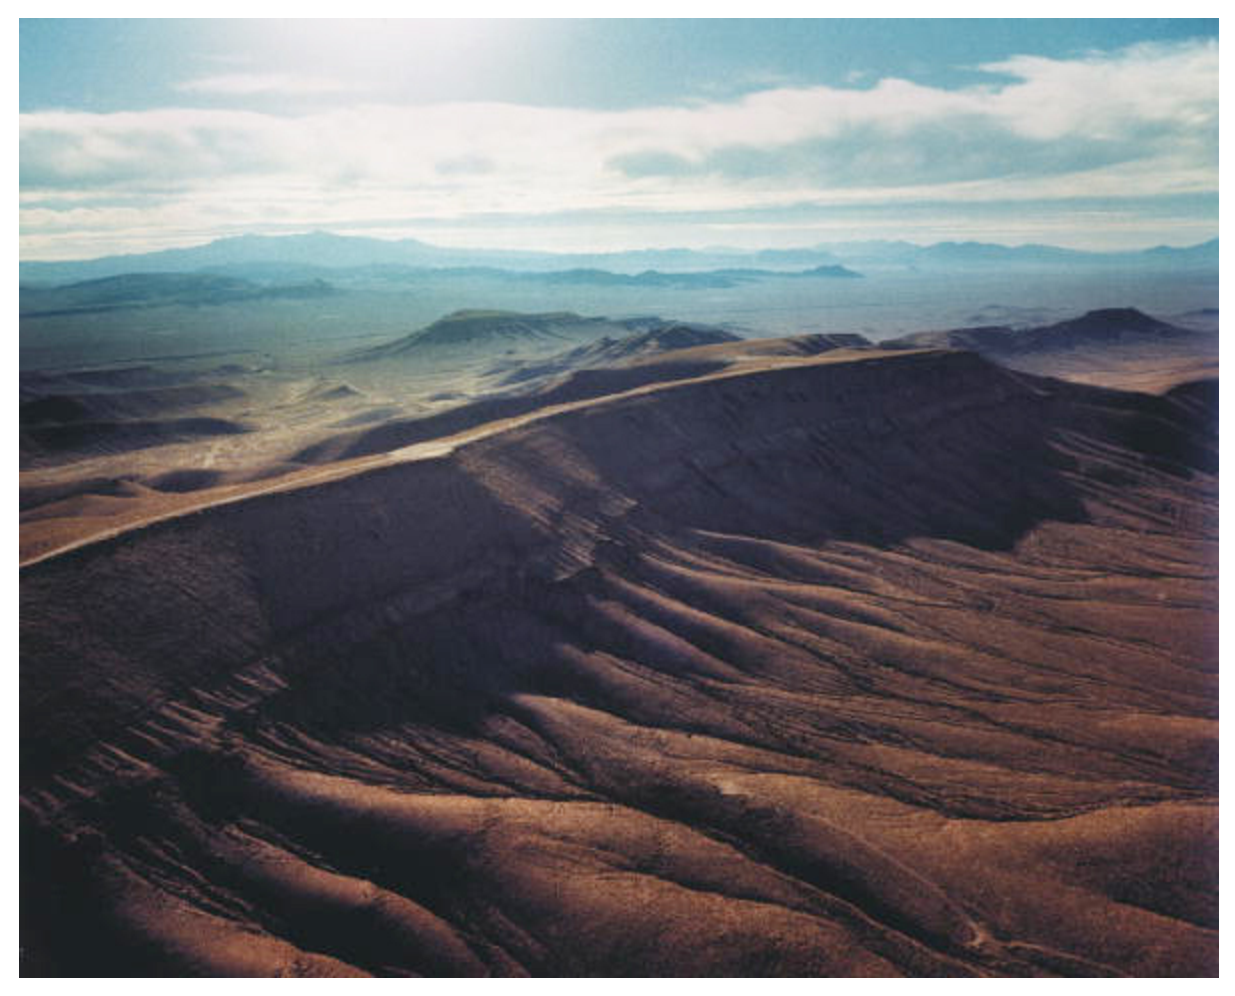
\includegraphics[width=0.5\textwidth]{./images/yucca_site.eps}
  \end{center}
  \caption{Yucca Mountain is in southern Nevada \cite{omb_yucca_2006}.}
  \label{fig:yucca_site}
\end{figure}

  }
\end{frame}

\begin{frame}[ctb!]
  \frametitle{Alternative Disposal Geology Options}
   \begin{minipage}{0.44\textwidth}
     \begin{figure}[h!]
         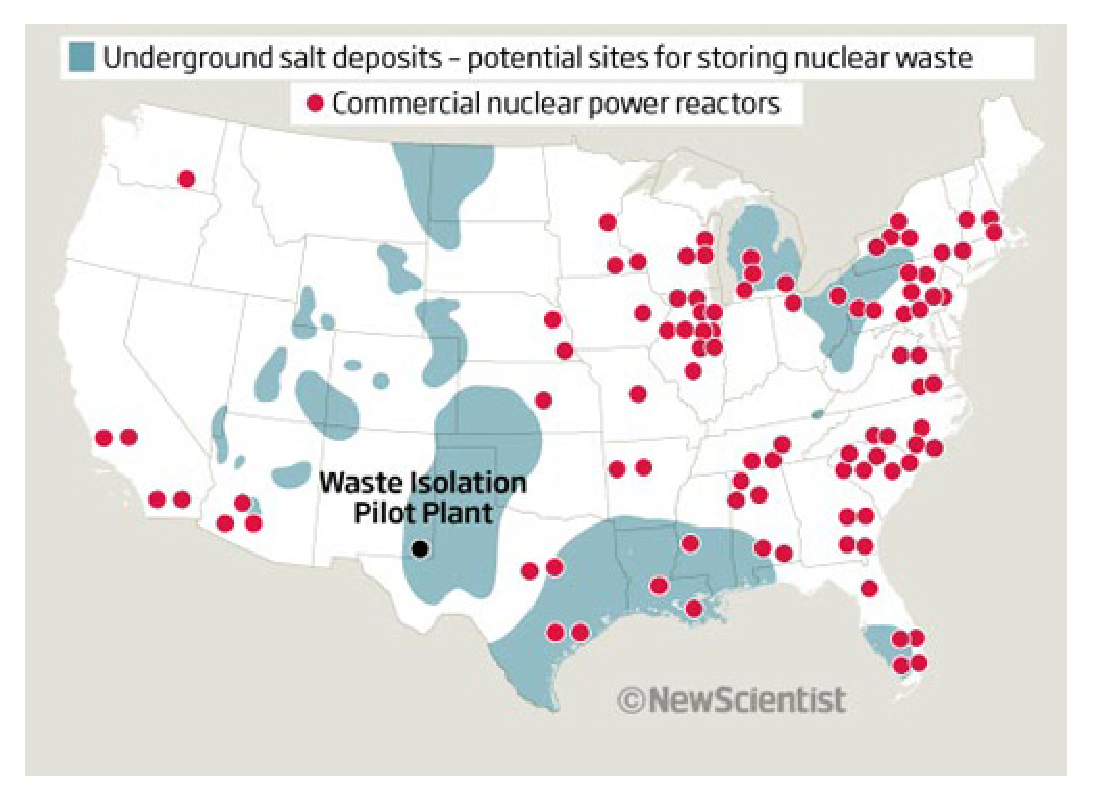
\includegraphics[width=0.8\textwidth]{./images/saltNewScientist.eps}
         \caption{U.S. Salt Deposits, ref. \cite{newscientist_where_2011}.}
     \end{figure}
     \begin{figure}[h!]
         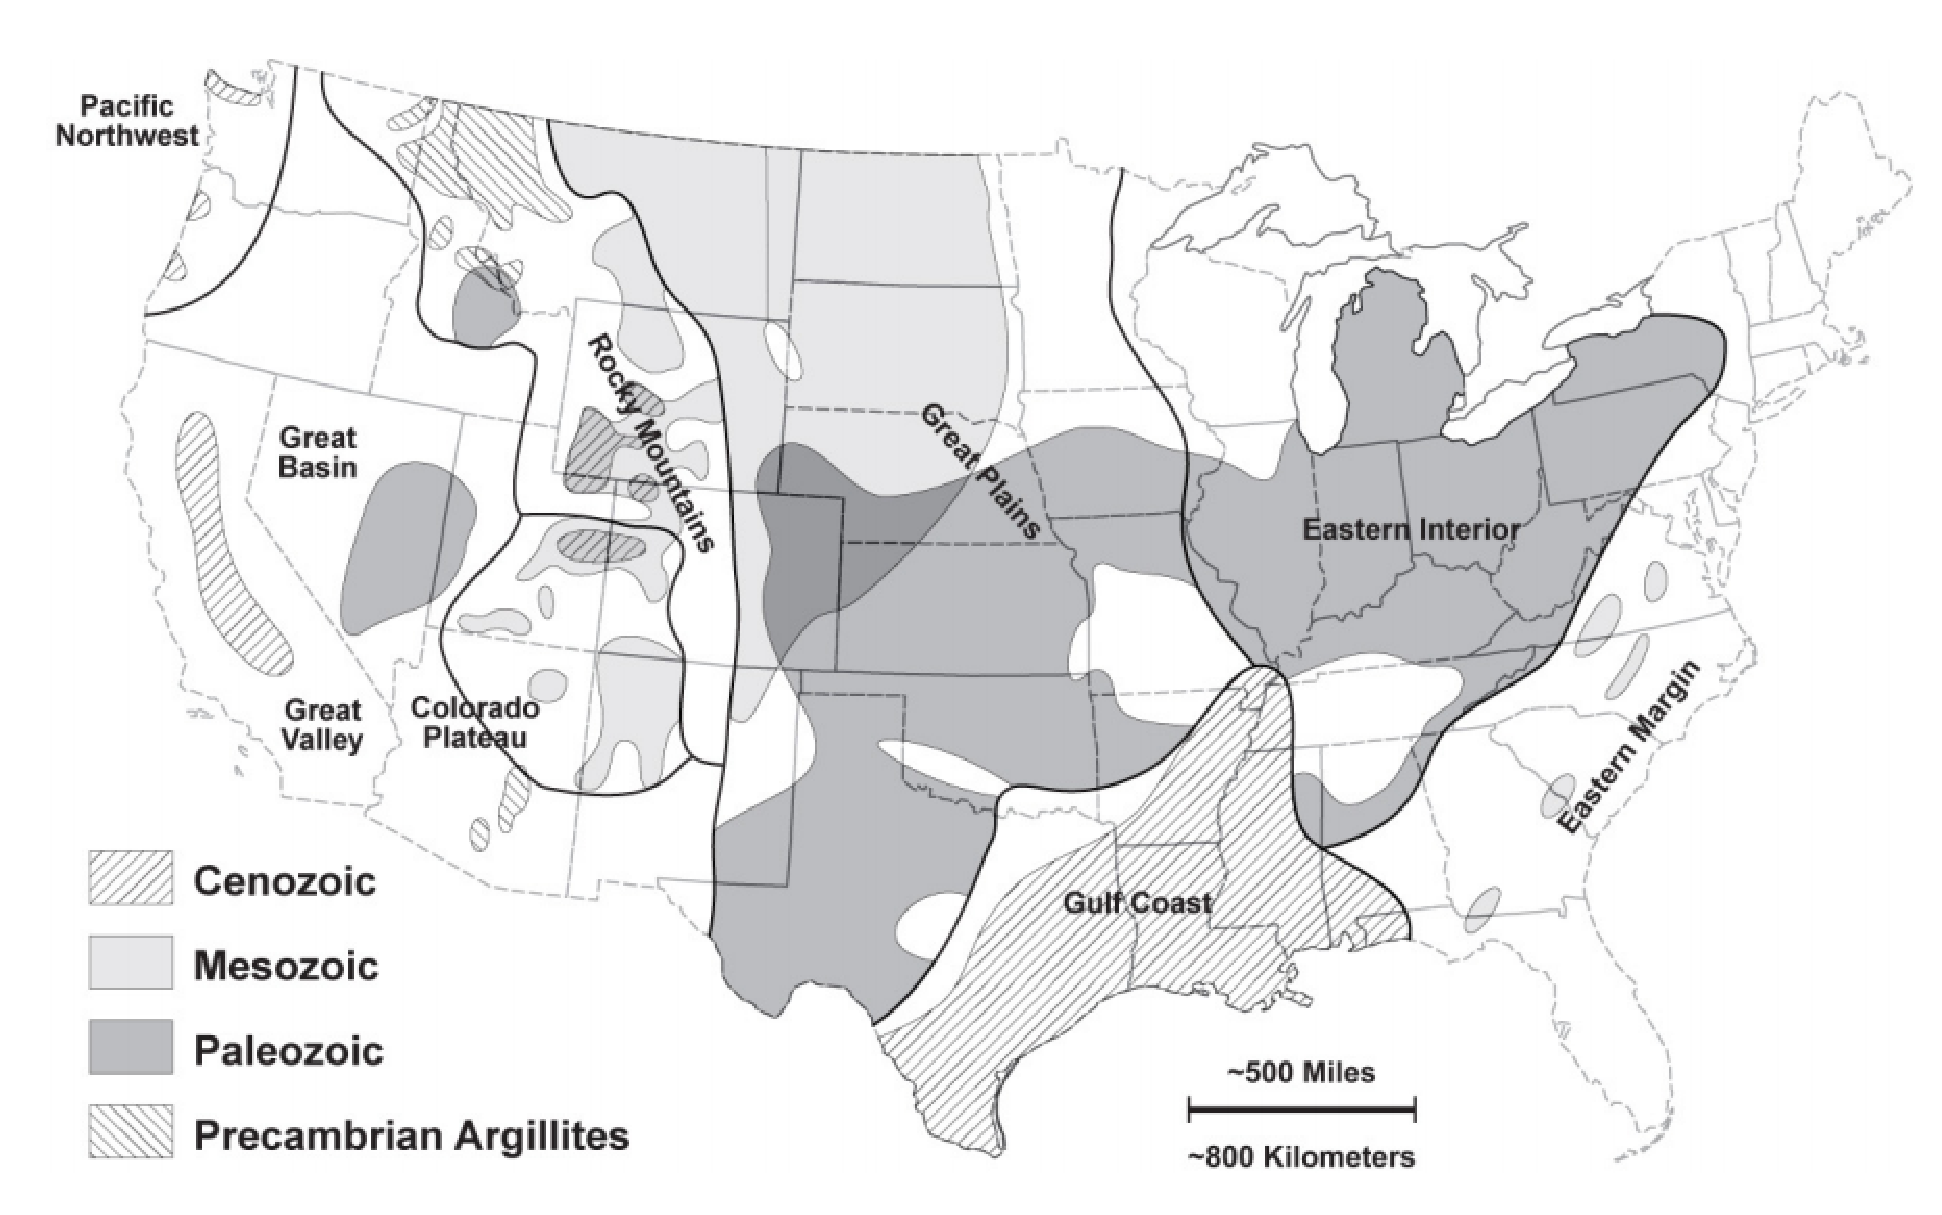
\includegraphics[width=0.8\textwidth]{./images/clayGonzales.eps}
         \caption{U.S. Clay Deposits, ref. \cite{gonzales_shales_1985}.}
     \end{figure}
   \end{minipage}
   \hspace{0.01cm}
   \begin{minipage}{0.44\textwidth}
     \begin{figure}[h!]
         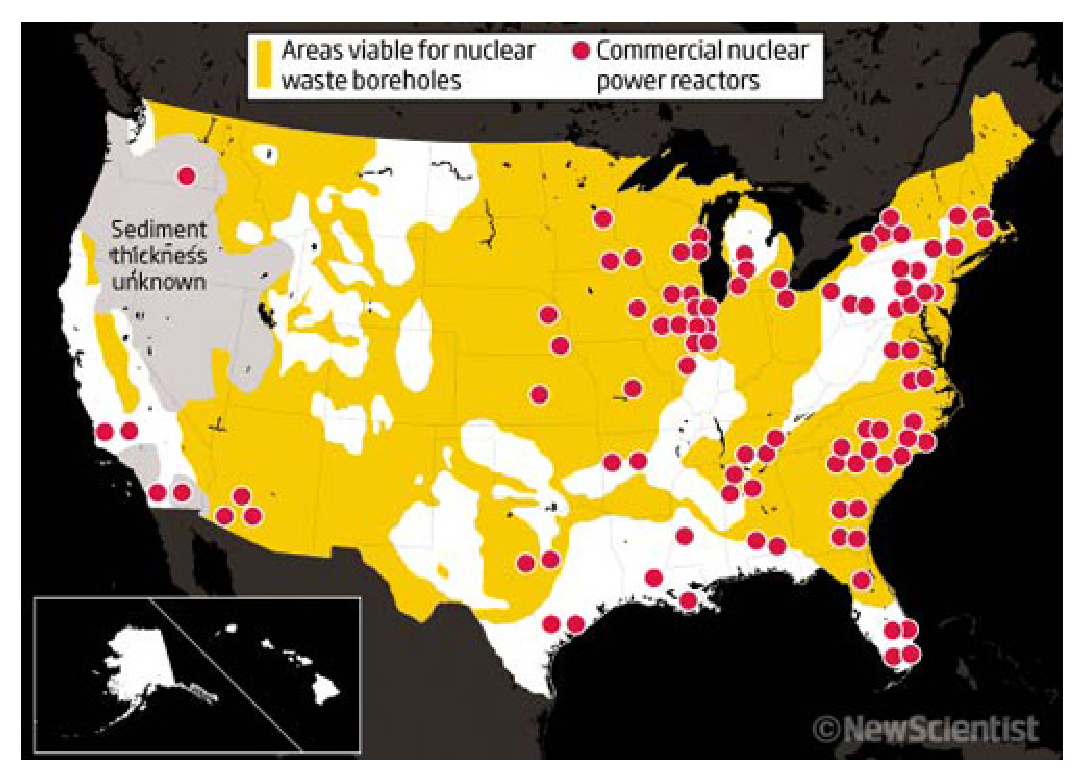
\includegraphics[width=0.8\textwidth]{./images/boreholeNewScientist.eps}
         \caption{U.S. Crystalline Basement, ref.  \cite{newscientist_where_2011}.}
     \end{figure}
     \begin{figure}[h!]
         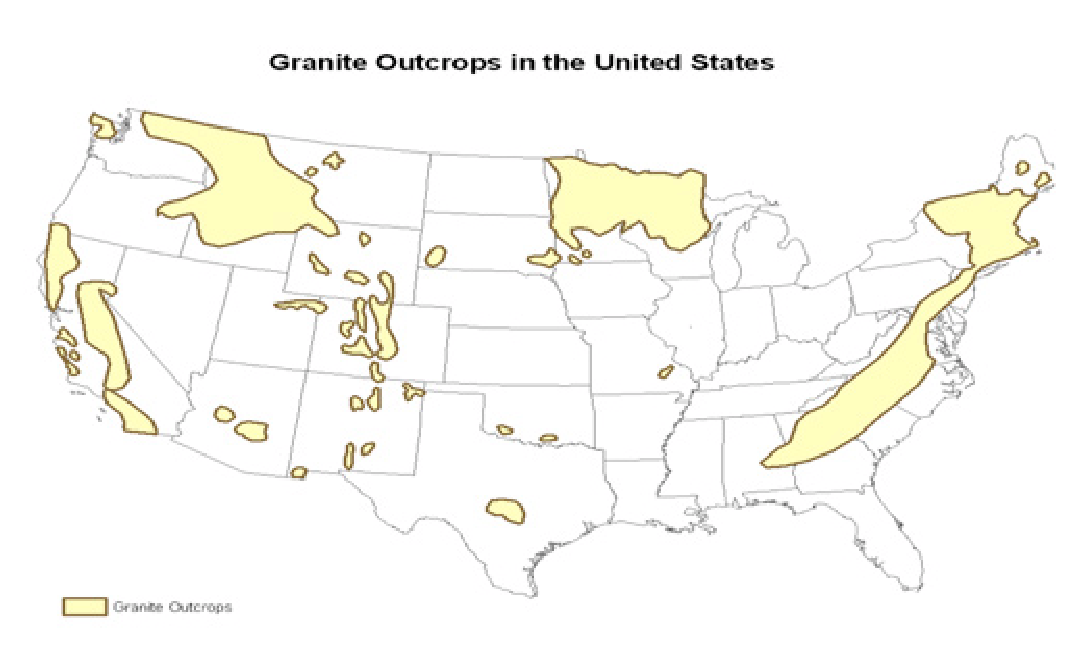
\includegraphics[width=0.8\textwidth]{./images/graniteBush.eps}
         \caption{U.S. Granite Beds, ref. \cite{bush_economic_1976}.}
     \end{figure}
   \end{minipage}
\end{frame}

\begin{frame}[ctb!]
  \frametitle{Clay Disposal Environments}
  \footnotesize{

  \begin{figure}[h!]
    \begin{center}
      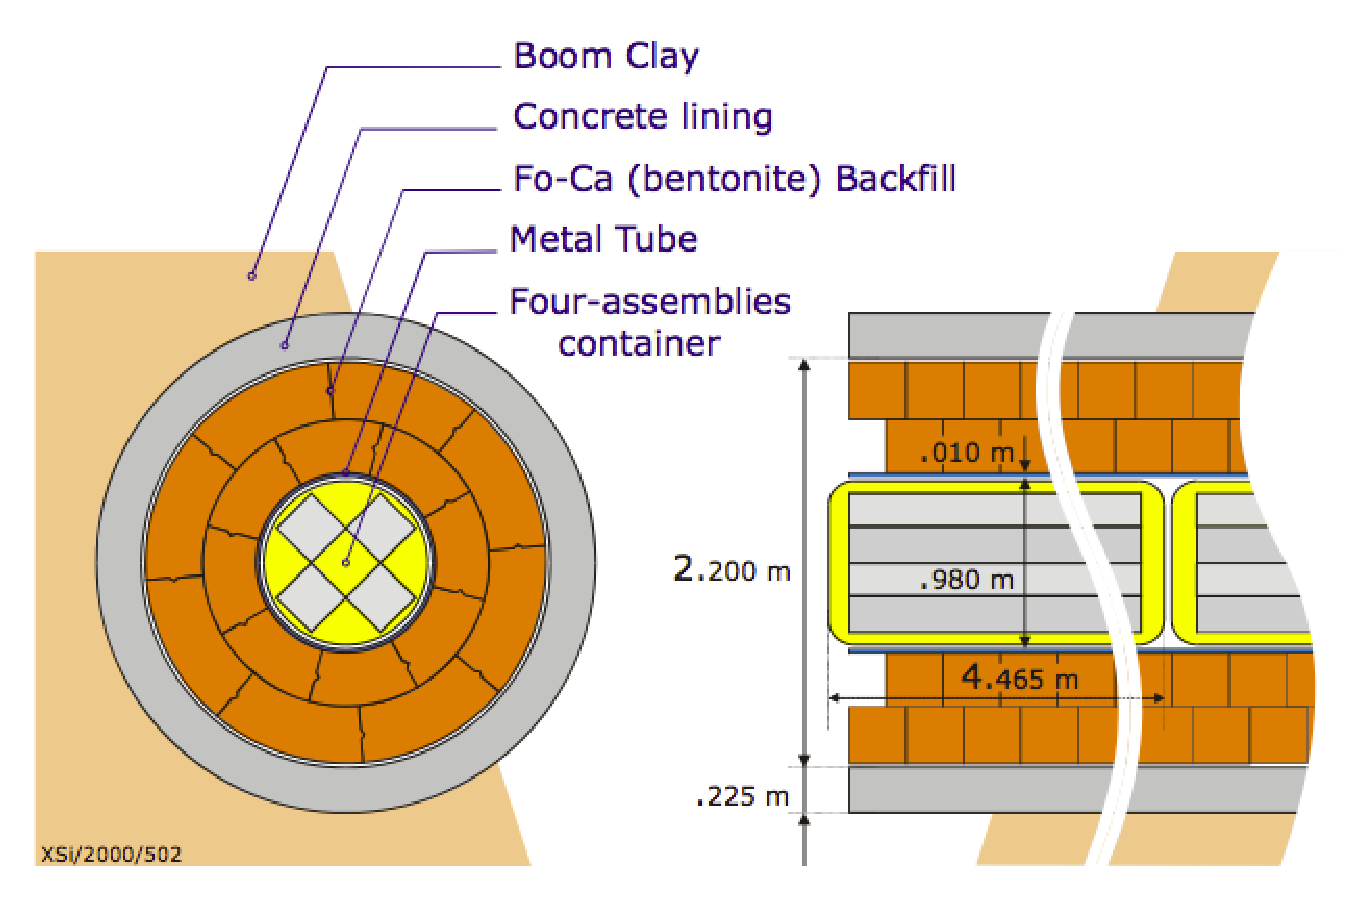
\includegraphics[height=.7\textheight]{./images/belgianClayRedImp.eps}
    \end{center}
    \caption{Belgian reference concept in Boom Clay 
    \cite{von_lensa_red-impact_2008}.}
    \label{fig:belgianClayRedImp}
  \end{figure}

}
\end{frame}

\begin{frame}[ctb!]
  \frametitle{Granite Disposal Environments}
  \footnotesize{

  \begin{figure}[h!]
    \begin{center}
      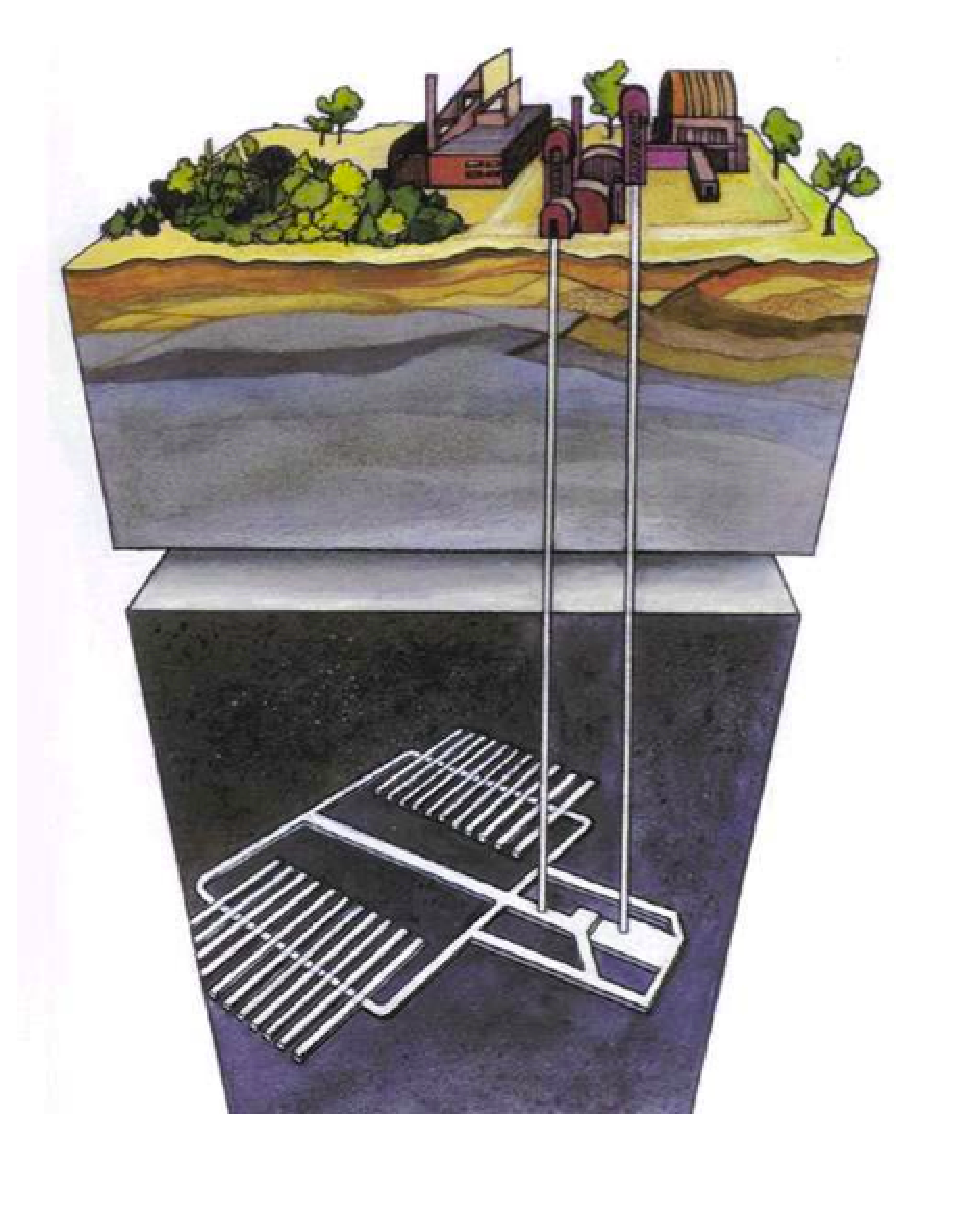
\includegraphics[height=.7\textheight]{./images/czechGraniteRedImp.eps}
    \end{center}
    \caption{Czech reference concept in Granite 
    \cite{von_lensa_red-impact_2008}.}
    \label{fig:czechGraniteRedImp}
  \end{figure}
}
\end{frame}

\begin{frame}[ctb!]
  \frametitle{Salt Disposal Environments}
  \footnotesize{

  \begin{figure}[h!]
    \begin{center}
      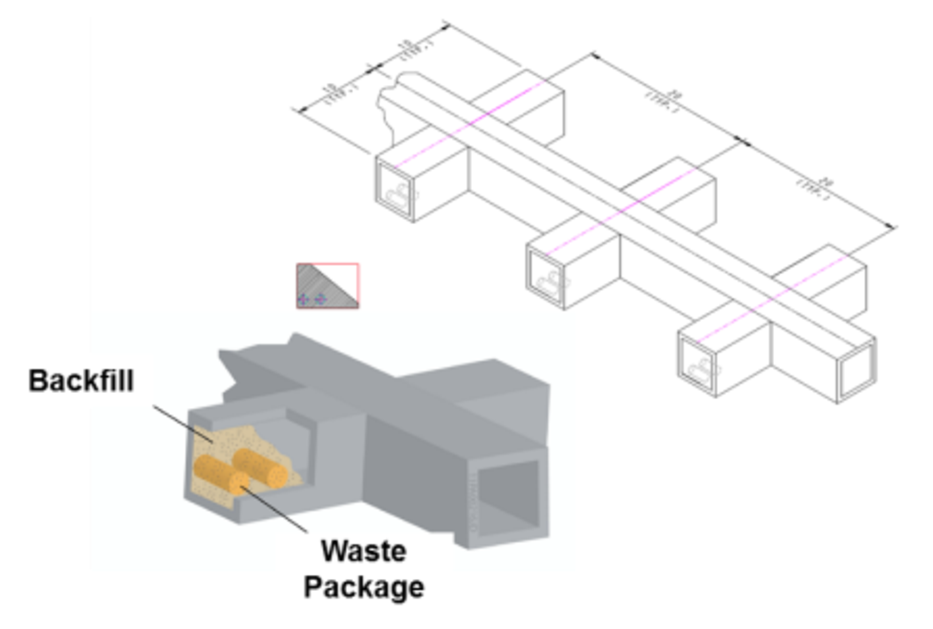
\includegraphics[height=.7\textheight]{./images/carter_salt_layout.eps}
    \end{center}
    \caption{DOE-NE Used Fuel Disposition Campaign  concept in 
    Salt \cite{hardin_generic_2011}.}
    \label{fig:salt_layout}
  \end{figure}
}
\end{frame}
\begin{frame}[ctb!]
  \frametitle{Salt Disposal Environments}
  \footnotesize{

  \begin{figure}[h!]
    \begin{center}
      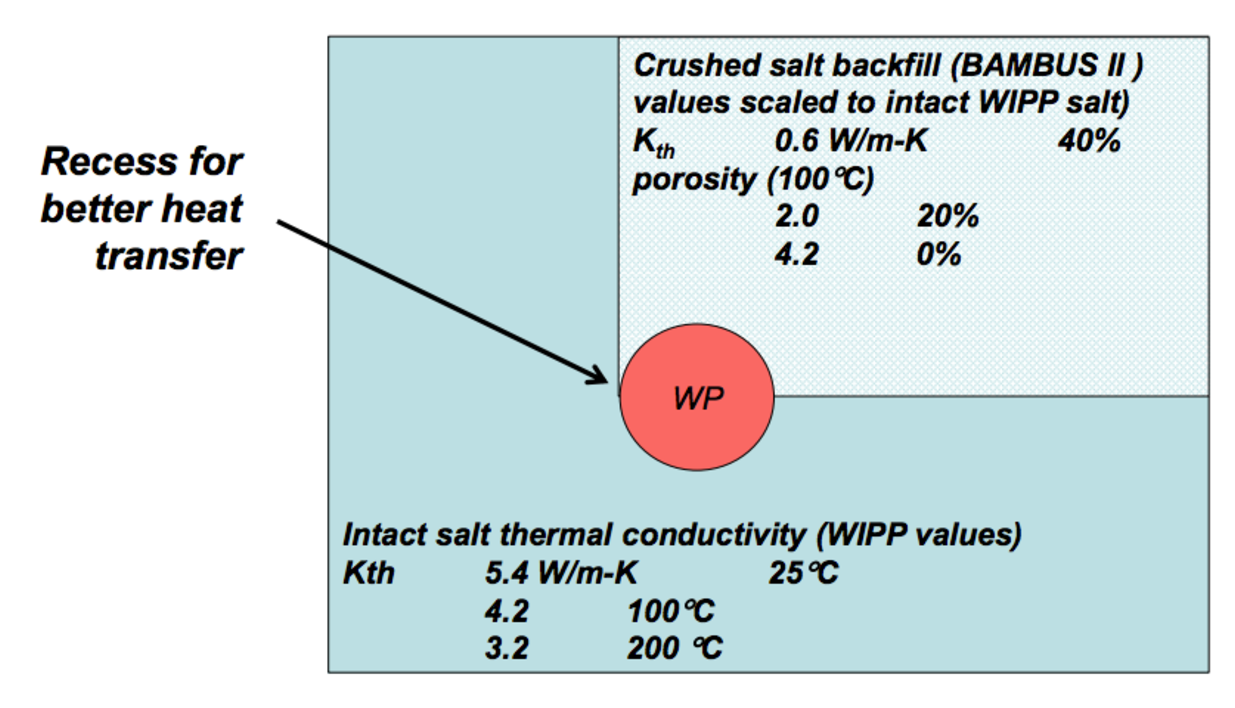
\includegraphics[height=.7\textheight]{./images/hardin_salt_layout.eps}
    \end{center}
    \caption{DOE-NE Used Fuel Disposition Campaign  concept in 
    Salt \cite{hardin_generic_2011}.}
    \label{fig:hardin_salt_layout}
  \end{figure}
}
\end{frame}

\begin{frame}[ctb!]
  \frametitle{Deep Borehole Disposal Environment}
  \footnotesize{

  \begin{figure}[h!]
    \begin{center}
      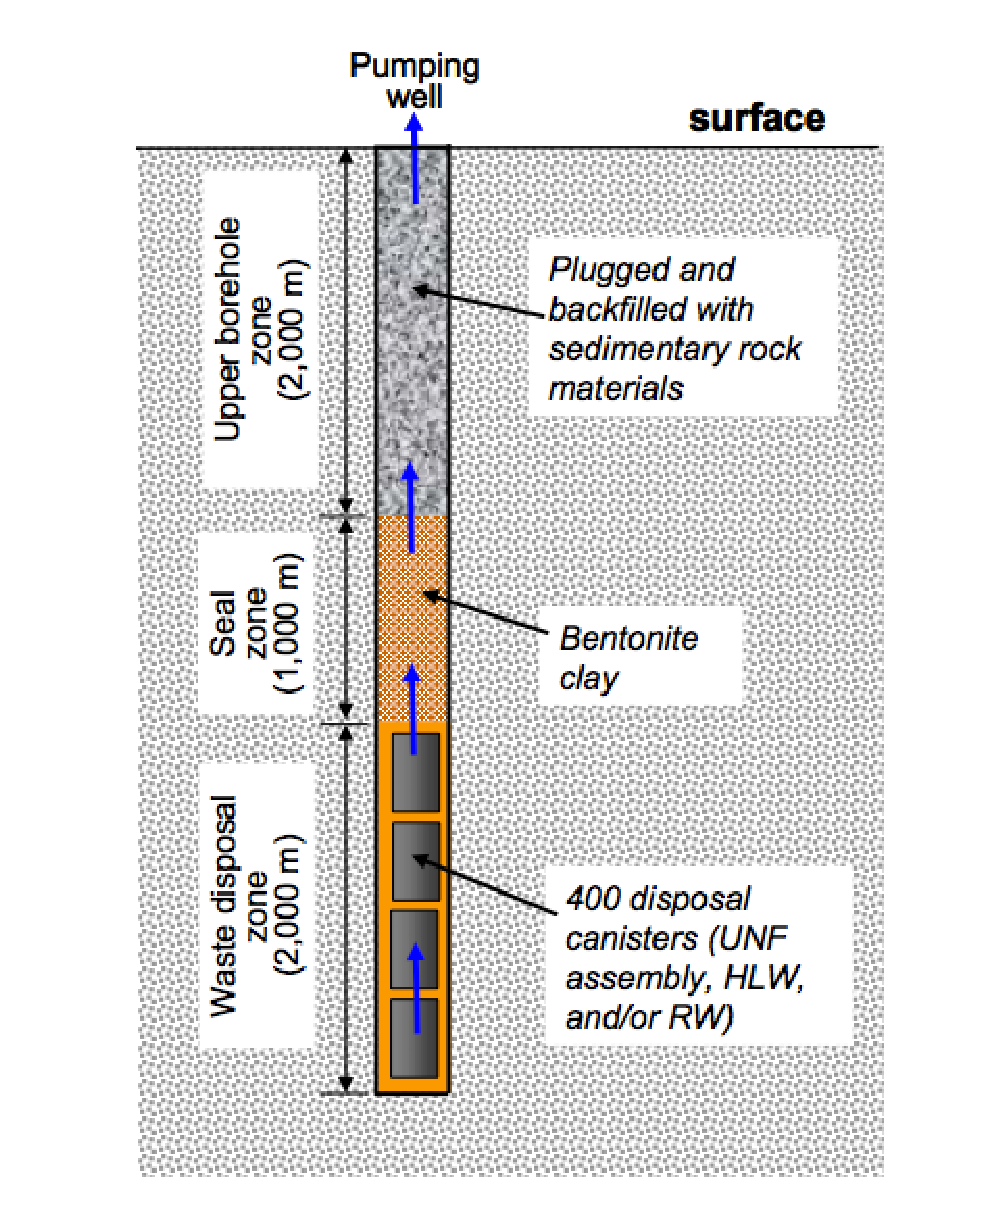
\includegraphics[height=.7\textheight]{./images/boreholeGPAM.eps}
    \end{center}
    \caption{DOE-NE Used Fuel Disposition Campaign Deep Borehole concept 
    \cite{hardin_generic_2011}.}
    \label{fig:boreholeGPAM}
  \end{figure}
}
\end{frame}




%%----------------------------------------%%
\begin{frame}[ctb!]
  \frametitle{Repository Components}
\footnotesize{
  \begin{figure}[htbp!]
  \begin{center}
    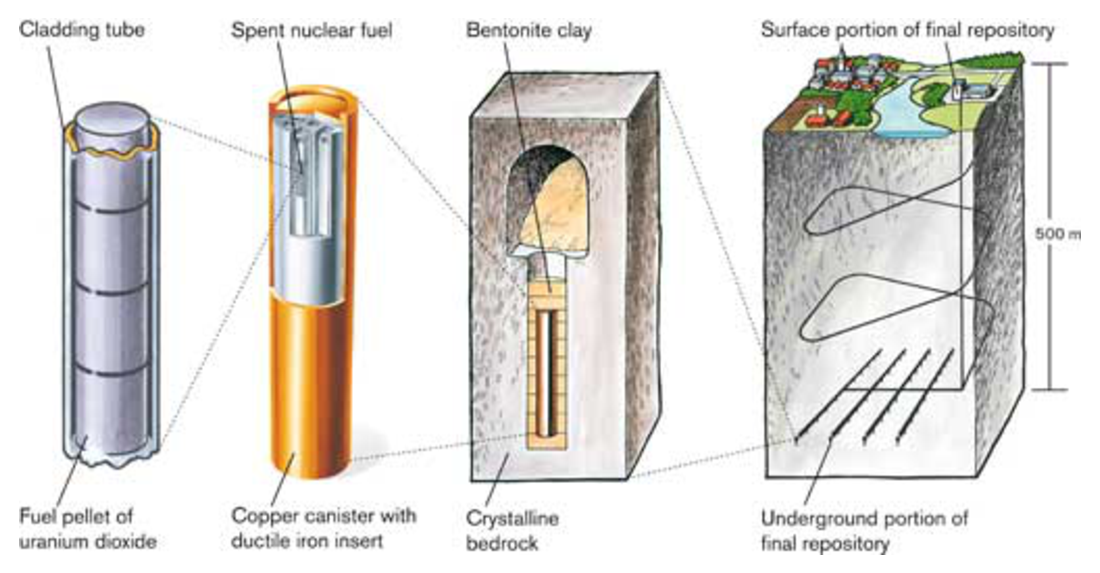
\includegraphics[width=0.7\textwidth]{./images/skb_components.eps}
  \end{center}
  \caption{Geologic disposal systems typically employ engineered barrier 
    systems as well as natural barrier systems. This is a Swedish concept in 
    granite \cite{ab_long-term_2006}.}
  \label{fig:skb_components}
\end{figure}

}
\end{frame}

%%----------------------------------------%%
\begin{frame}[ctb!]
  \frametitle{Engineered Barriers : Waste Forms}
\footnotesize{
  The first line of defense is the waste form.
  \begin{figure}[htbp!]
  \begin{center}
    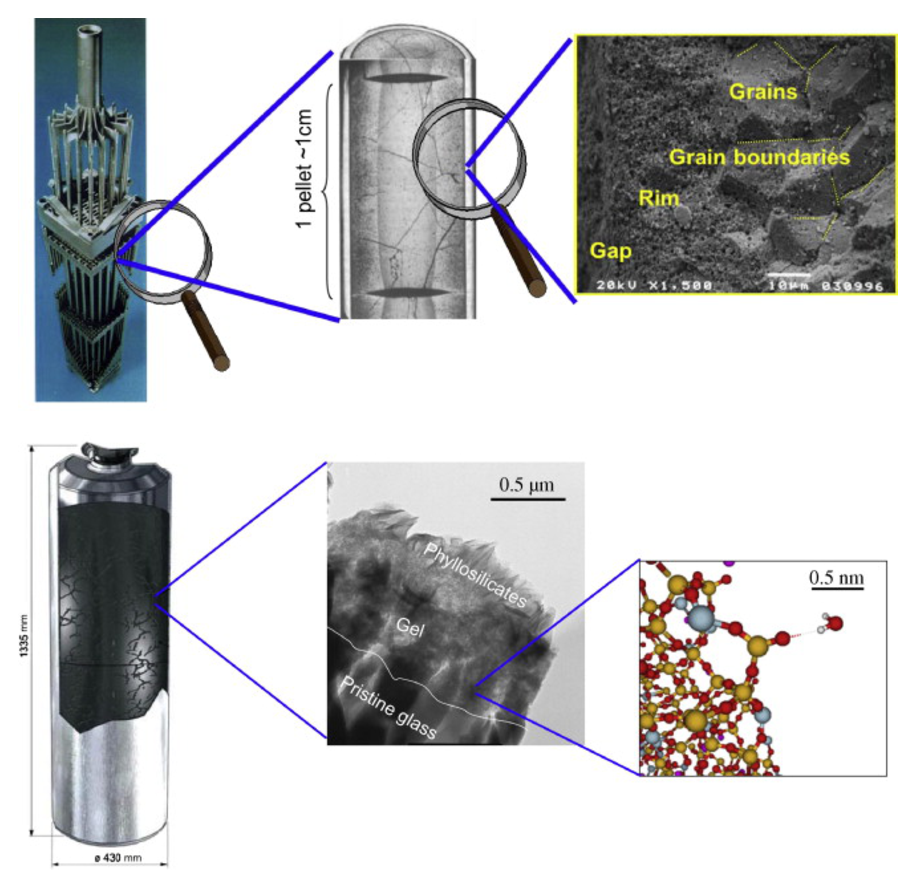
\includegraphics[width=0.5\textwidth]{./images/waste_forms_poinssot.eps}
  \end{center}
  \caption{A comparison of uranium oxide and borosilicate glass waste forms 
  \cite{poinssot_long-term_2012}.}
  \label{fig:waste_forms_poinssot}
\end{figure}

}
\end{frame}

%%----------------------------------------%%
\begin{frame}[ctb!]
  \frametitle{Engineered Barriers : Waste Packages}
\footnotesize{
  \begin{figure}[htbp!]
  \begin{center}
    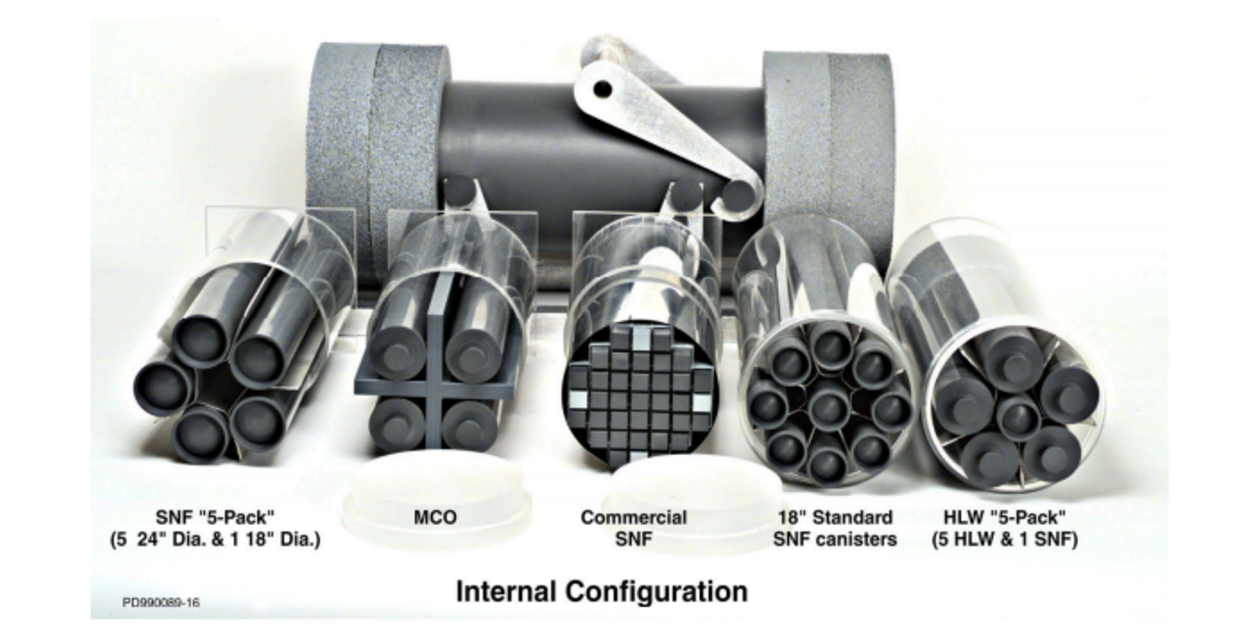
\includegraphics[width=0.7\textwidth]{./images/packages_ineel.eps}
  \end{center}
  \caption{Conceptual mockup of waste packages around waste forms 
    \cite{bridges_standardized_2001}.}
  \label{fig:packages}
\end{figure}

}
\end{frame}

%%----------------------------------------%%
\begin{frame}[ctb!]
  \frametitle{Engineered Barriers : Disposal Cask}
\footnotesize{
  \begin{figure}[htbp!]
  \begin{center}
    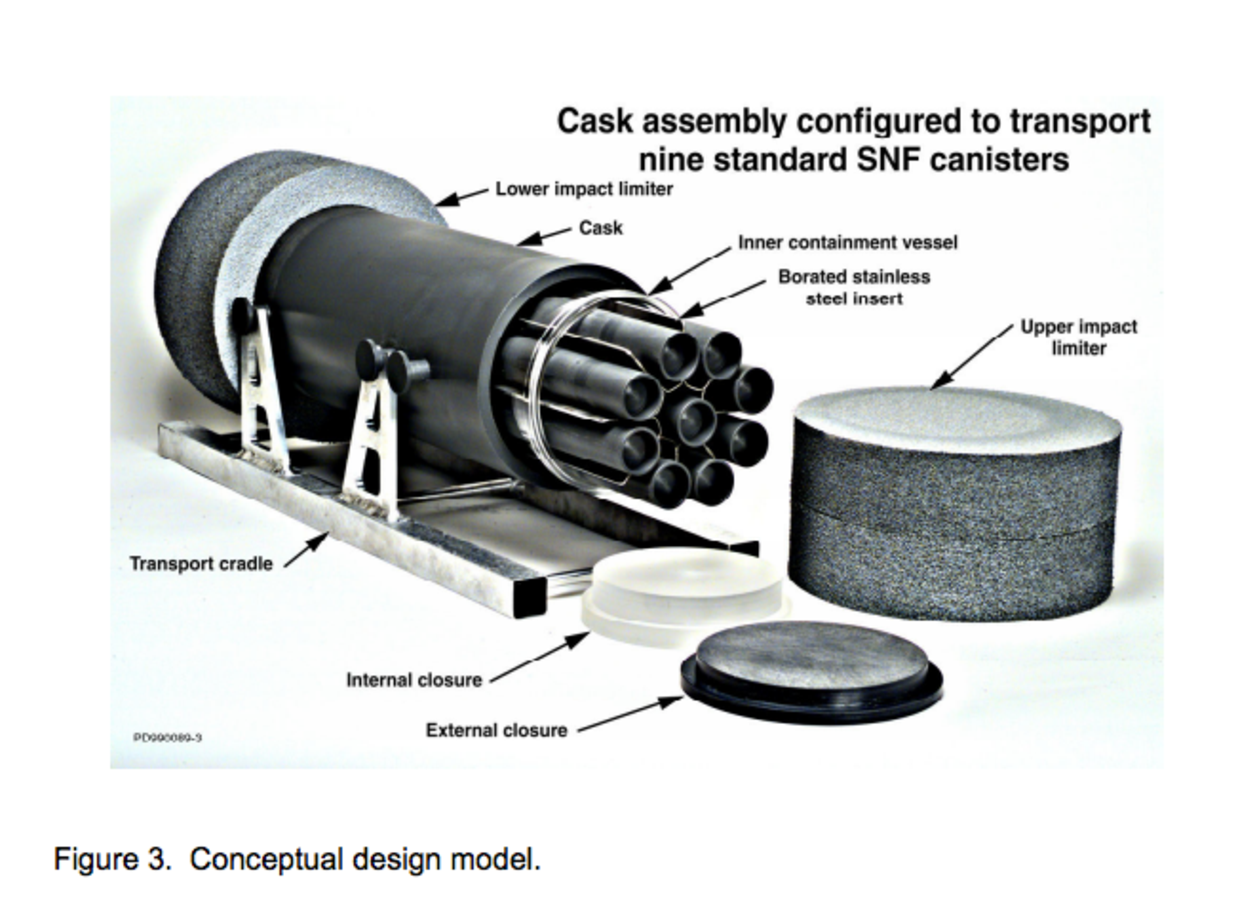
\includegraphics[width=0.7\textwidth]{./images/cask_ineel.eps}
  \end{center}
  \caption{Conceptual mockup of a transport and disposal cask 
    \cite{bridges_standardized_2001}.}
  \label{fig:packages}
\end{figure}

}
\end{frame}

%%----------------------------------------%%
\begin{frame}[ctb!]
  \frametitle{Engineered Barriers : Tunnel}
\footnotesize{
  \begin{figure}[htbp!]
  \begin{center}
    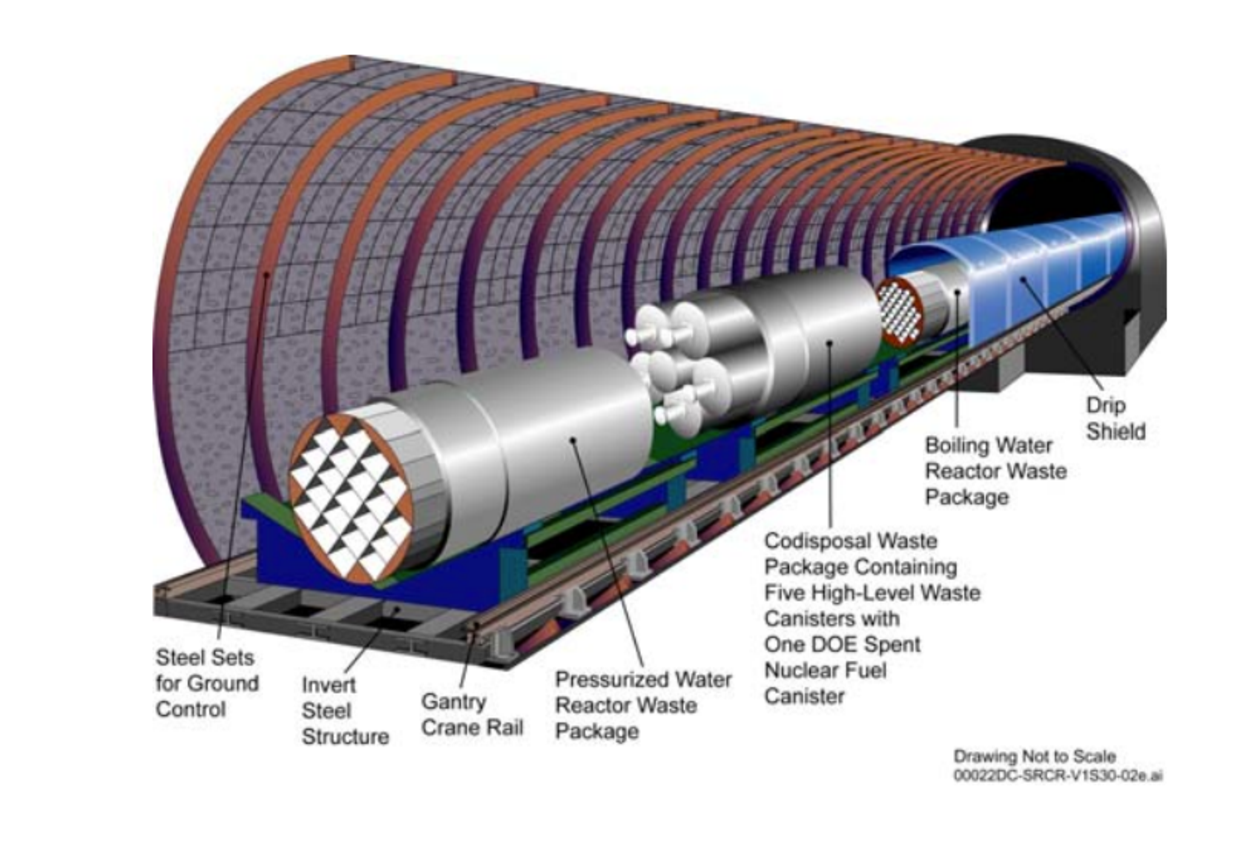
\includegraphics[height=0.7\textwidth]{./images/yucca_tunnel.eps}
  \end{center}
  \caption{The current U.S. geologic disposal concept \cite{peters_whats_2013}.}
  \label{fig:yucca_tunnel}
\end{figure}

}
\end{frame}

%%----------------------------------------%%
\begin{frame}[ctb!]
  \frametitle{Natural Barrier : Geology}
\footnotesize{
  \begin{figure}[htbp!]
  \begin{center}
    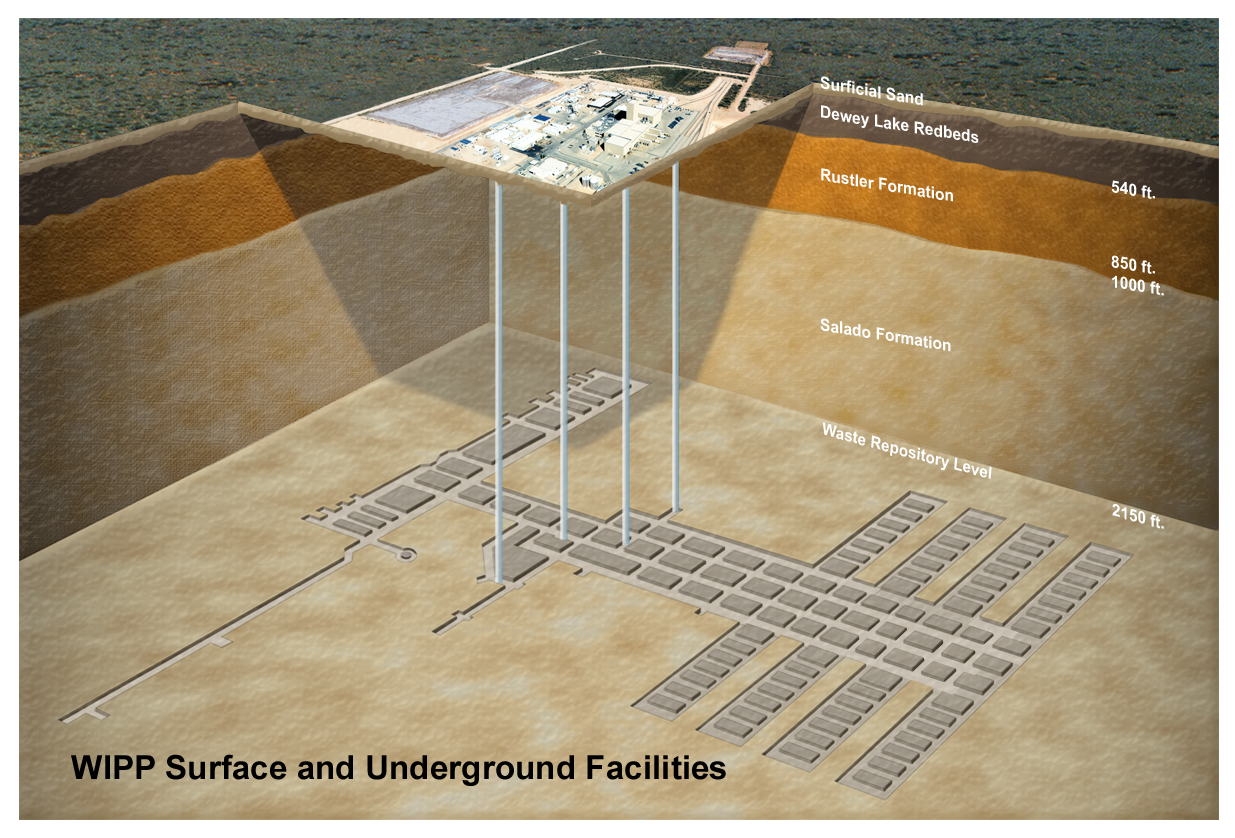
\includegraphics[width=0.7\textwidth]{./images/wipp_stratigraph.eps}
  \end{center}
  \caption{The Waste Isolation Pilot Plant has many geologic layers above the 
    salt bed \cite{doe_wipp_2013}.}
  \label{fig:wipp}
\end{figure}

}
\end{frame}

\begin{frame}
  \frametitle{Repository Layouts}

  \begin{minipage}{0.49\textwidth}
    \begin{figure}[h!]
      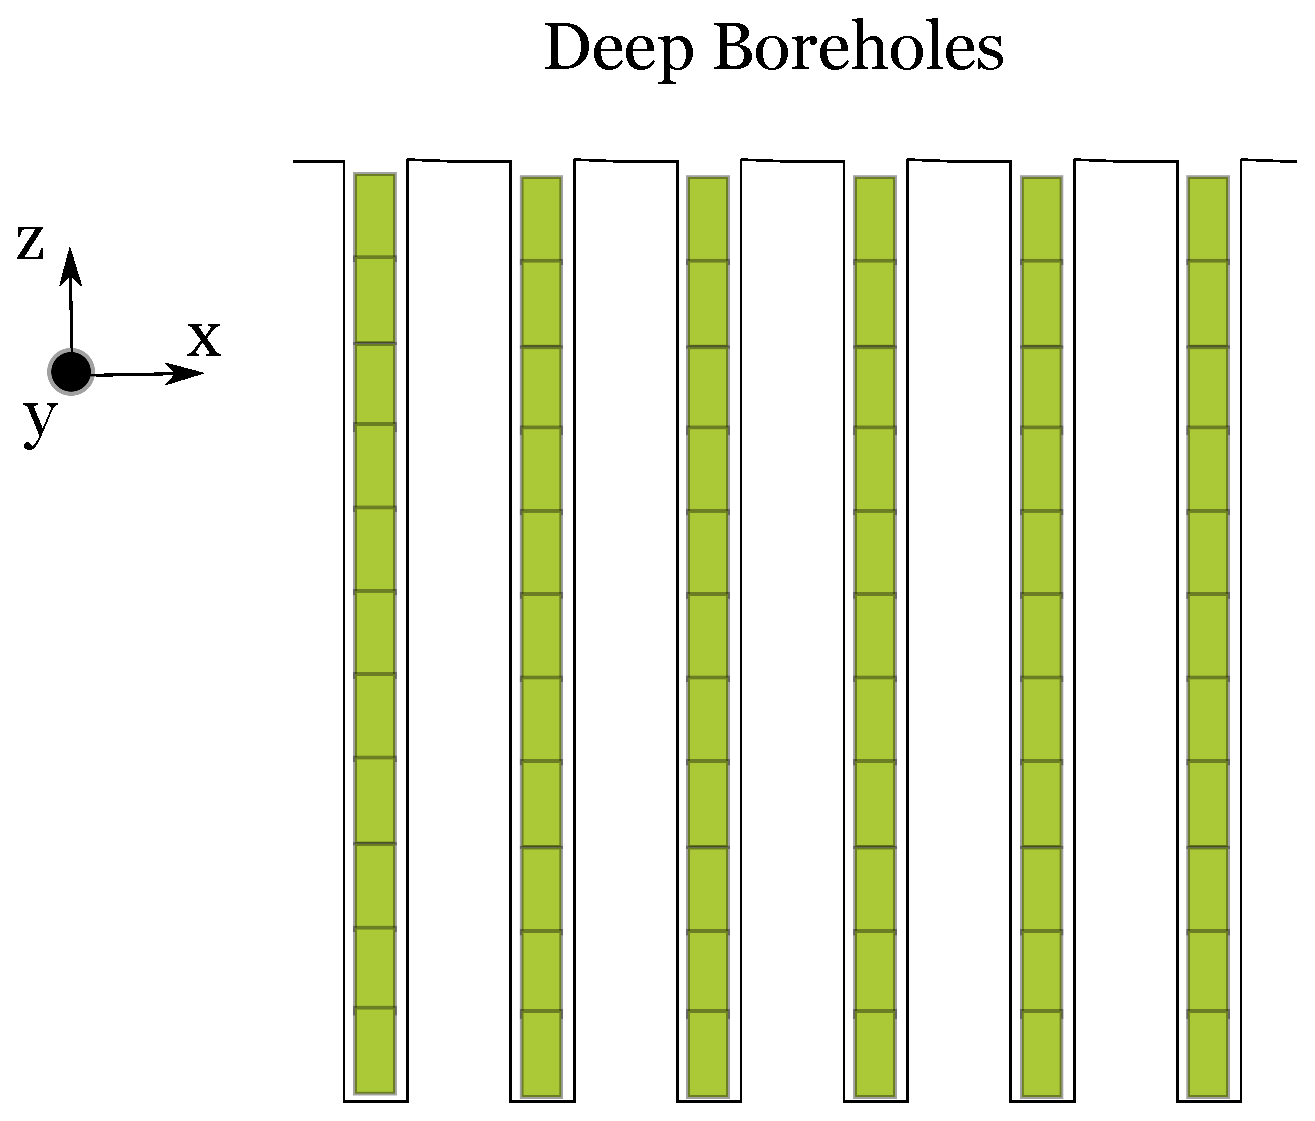
\includegraphics[width=0.75\textwidth]{./images/boreholes.eps}
    \end{figure}
    \begin{figure}[h!]
      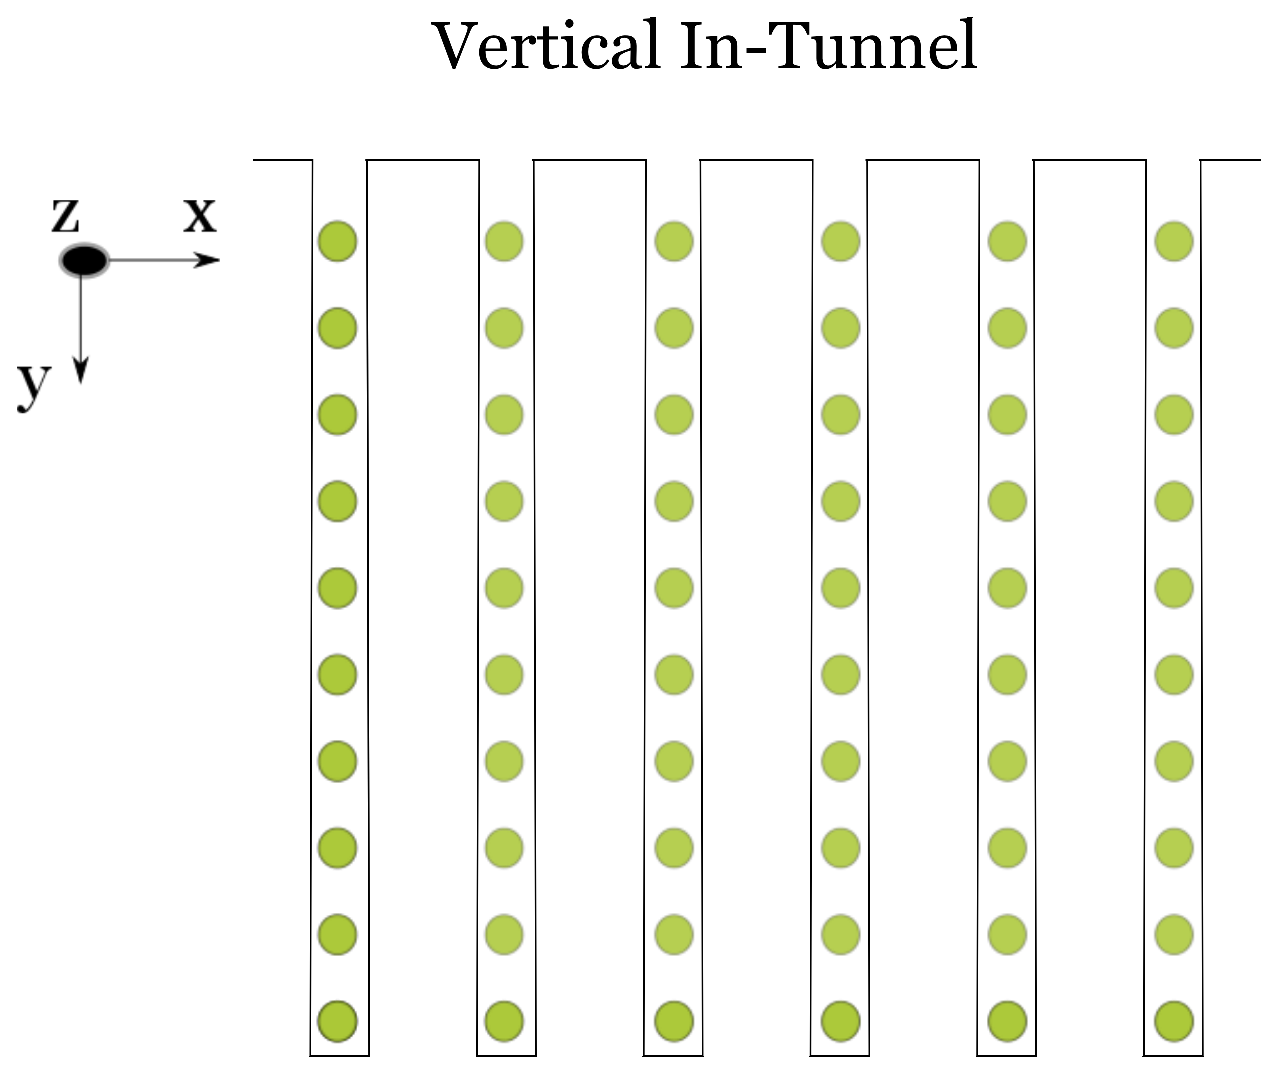
\includegraphics[width=0.75\textwidth]{./images/vertical.eps}
    \end{figure}
  \end{minipage}
  \hspace{0.01cm}
  \begin{minipage}{0.49\textwidth}
    \begin{figure}[h!]
      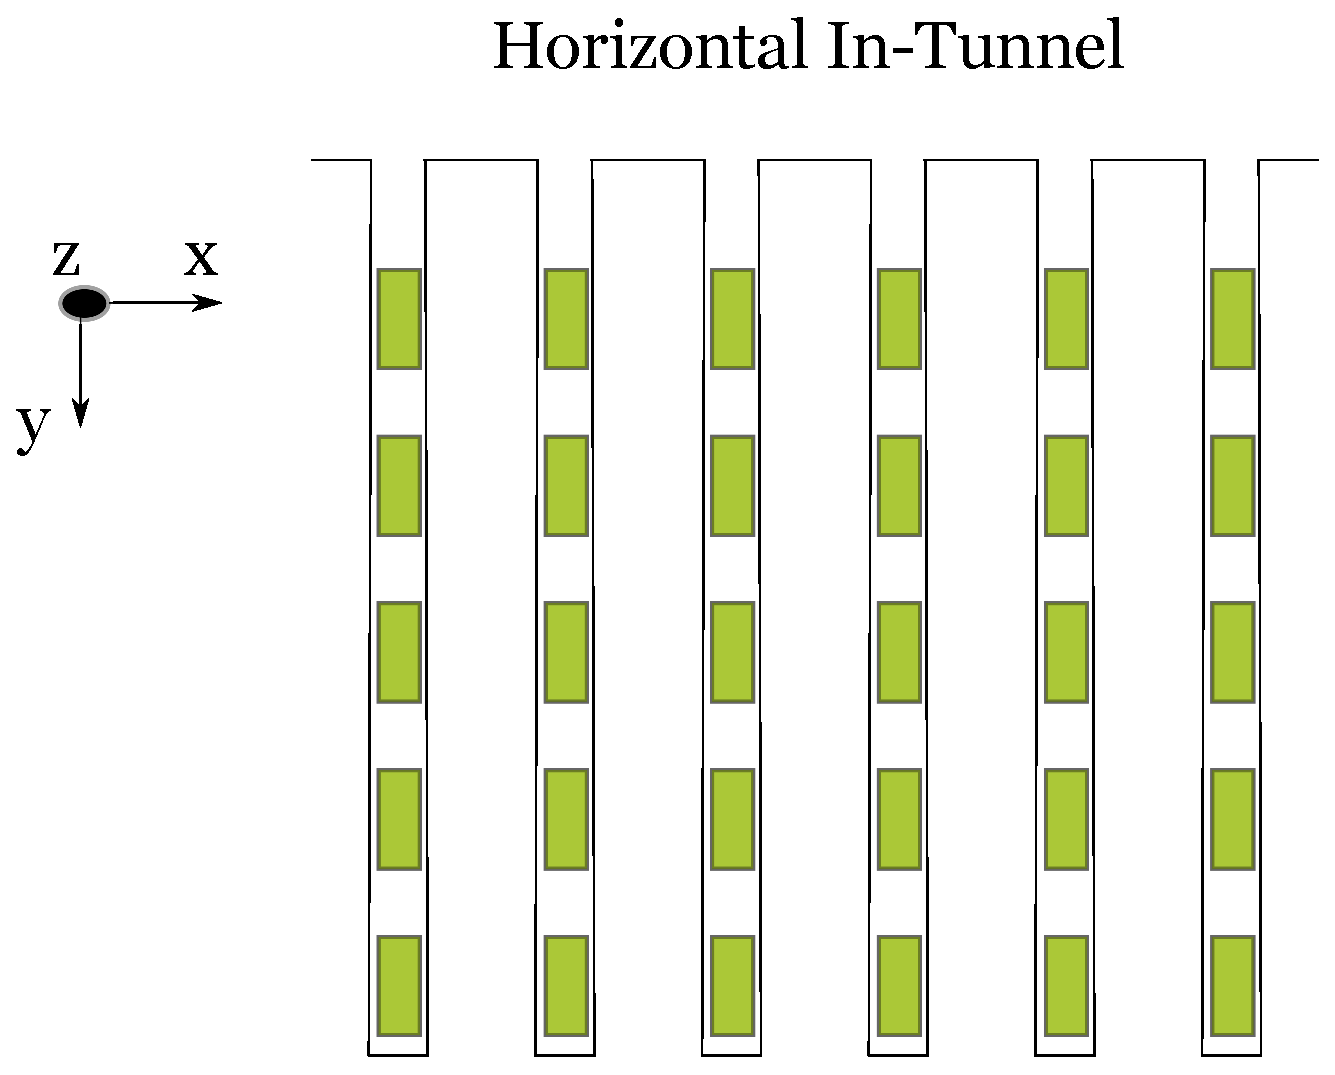
\includegraphics[width=0.8\textwidth]{./images/horizontal.eps}
    \end{figure}
    \begin{figure}[h!]
      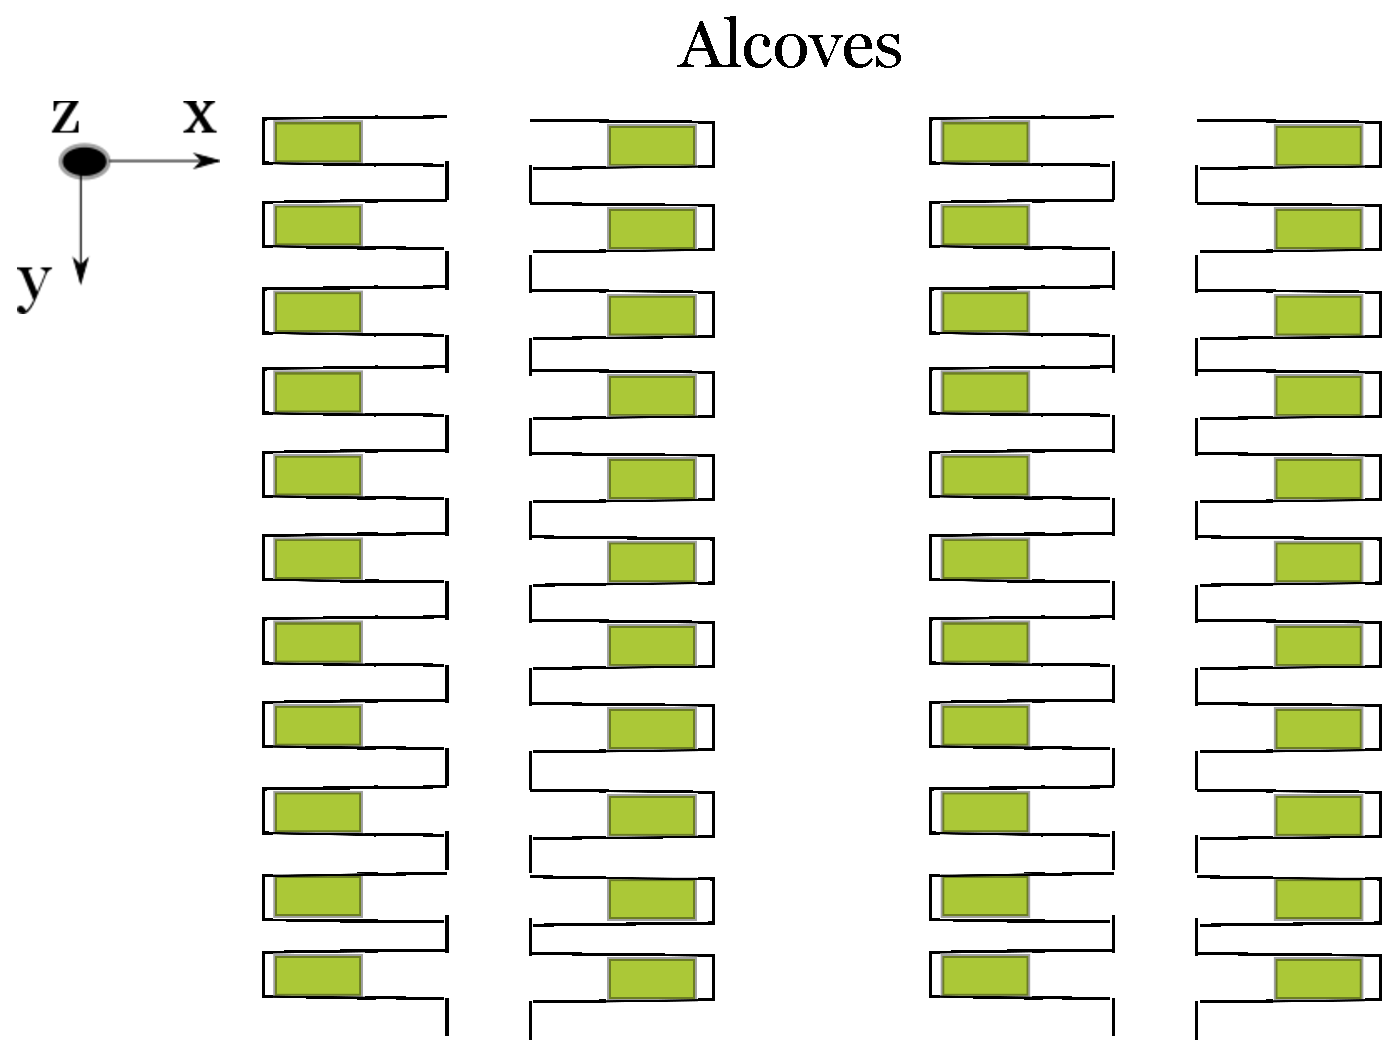
\includegraphics[width=0.8\textwidth]{./images/alcoves.eps}
    \end{figure}
  \end{minipage}

\end{frame}


\subsection{Fuel Cycle Simulator Capabilities}


% They just report mass flows
% or are proprietary and super long running

\begin{frame}[ctb!]
  \frametitle{Cyclus Top Level Fuel Cycle Simulator}
  % most only report mass flows.
  \begin{figure}[htbp!]
    \begin{center}
      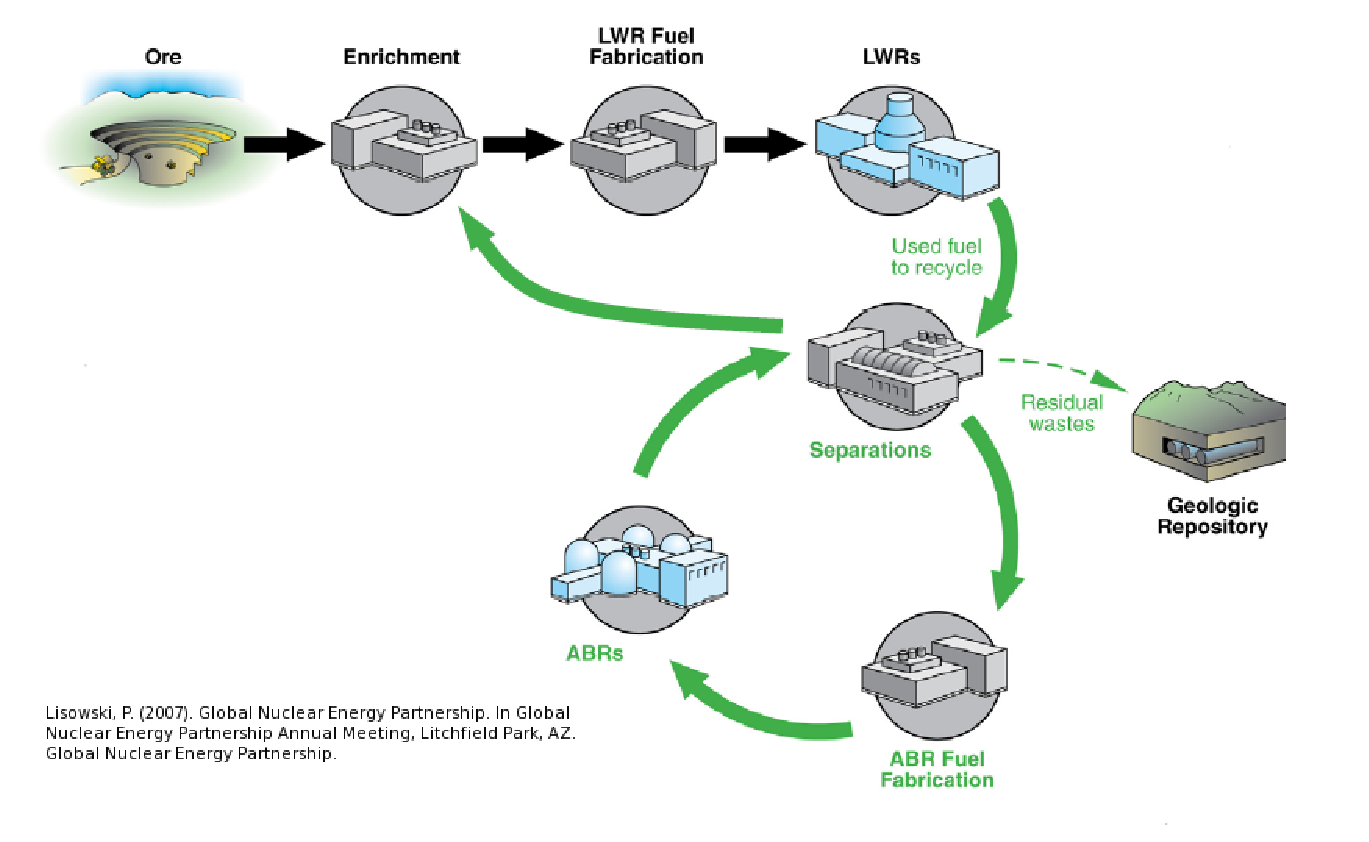
\includegraphics[height=3.5cm]{./images/simulations.eps}
    \end{center}
    \caption{Top level simulators are intended to model the collective 
    behavior of various fuel cycle decisions and 
    strategies \cite{lisowski_global_2007}.}
    \label{fig:simulation}
  \end{figure}
  \begin{figure}[htbp!]
    \begin{center}
      
\includegraphics[height=1cm]{./images/cycluslogo.eps}
    \end{center}
    \caption{ cyclus.github.com \cite{huff_cyclus_2013}.}
    \label{fig:simulation}
  \end{figure}
\end{frame}

\begin{frame}[ctb!]
  \frametitle{Need For an Integrated Repository Model}

  %        File: systools_tab.tex
%     Created: Mon Aug 29 09:00 AM 2011 C
% Last Change: Mon Aug 29 09:00 AM 2011 C
%
\begin{table}
  \centering
  \footnotesize{
  \begin{tabular}{|l|l|c|c|c|}
    \multicolumn{5}{c}{\textbf{Repository Capabilities within Systems Analysis Tools}}\\
    \hline
    Tool & Institution & Fuel Disposition & Radionuclide Transport & Heat Transport  \\
    \hline
    NUWASTE\cite{abkowitz_nuclear_2010} & NWTRB & yes & no & no \\
    VISION \cite{yacout_vision_2006} & INL   & yes & no & YMR only \\
    DANESS \cite{van_den_durpel_daness:_2006} & ANL   & no & no & no \\
    COSI   \cite{boucher_international_2010} & CEA   & yes & no & yes \\
    NFCSim \cite{schneider_nfcsim_2004} & LANL  & no & no & no \\
    CAFCA  \cite{guerin_benchmark_2009} & MIT   & no & no & no \\
    ORION  \cite{guerin_benchmark_2009} & BNL   & no & no & no \\
    TSM    \cite{turner_discrete_2010} & OCRWM & yes & no & YMR only \\
    \hline
  \end{tabular}
  \caption[System Tools]{System tools are lacking in radionuclide transport and  
  heat transport calculations in generic geologic media.}
  \label{tab:systools}
  }
\end{table}




\end{frame}


\begin{frame}[ctb!]
\frametitle{Contributions from This Work}

This work has provided a platform capable of bridging the gap between fuel cycle 
simulation and repository performance analysis.

  \begin{itemize}
  \item Conducted thermal transport sensitivity analyses. \cite{huff_numerical_2012, huff_benchmarking_2012}
  \item Conducted contaminant transport sensitivity analyses. \cite{huff_key_2012}
  \item \Cyder acheived integration with a fuel cycle simulator.
  \item Abstracted physical models of thermal and contaminant transport. \cite{huff_hydrologic_2013}
  \item Demonstrated dominant physics of those models in \Cyder, integrated 
  with \Cyclus. \cite{huff_dynamic_2013, huff_cyclus_2013}
  \item Published source code, documentation, and testing to facilitate 
  extension by external developers. \cite{huff_cyder_2013}
  \end{itemize}
\end{frame}


\section{Modeling Paradigm}
\subsection{Cyder Overview}

\begin{frame}[ctb!]
  \frametitle{Cyder Paradigm : Modularity }
  A modular repository framework facilitates 
  \begin{itemize}
    \item  interchangable subcomponents 
    \item and simulations with varying levels of detail.
  \end{itemize}
 \pause
  Integration with a fuel cycle simulator facilitates
  \begin{itemize}
    \item analysis of feedback effects upon the fuel cycle
    \item and investigation of fuel cycle choices on disposal system 
      performance.
  \end{itemize}
\end{frame}


\begin{frame}[ctb!]
  \frametitle{Cyder Paradigm : Waste Stream Acceptance}
To participate in fuel cycle simulation, the repository model must accept 
\textbf{arbitrary} spent fuel and high level waste \textbf{material data 
objects} resulting from the Cyclus simulated fuel cycle.  

  \begin{figure}[htbp!]
    \begin{center}
      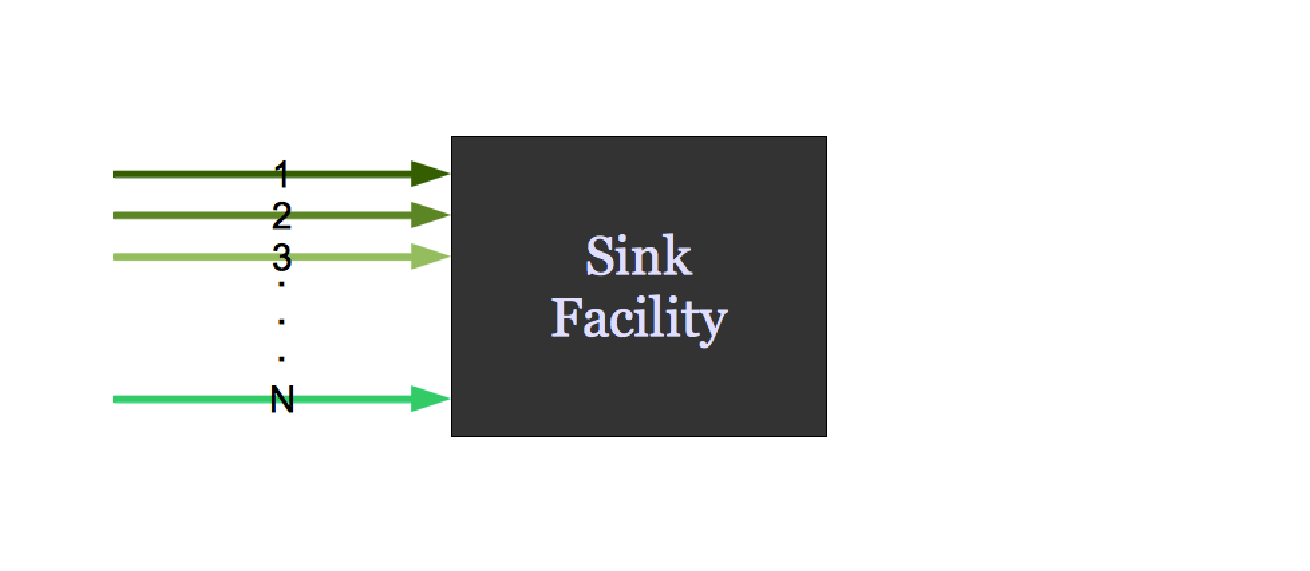
\includegraphics[height=5cm]{./images/sinkfacility.eps}
    \end{center}
    \caption{ The Cyder Facility dynamically accepts material from the 
    coupled fuel cycle simulation.} 
    \label{fig:sinkfacility}
  \end{figure}
% Sink Facility ?
\end{frame}

\begin{frame}[ctb!]
  \frametitle{Cyder Paradigm : Waste Stream Conditioning}
  \footnotesize{

    \textbf{Waste conditioning} is the process of packing a waste stream into an appropriate 
waste form. 
  
\begin{figure}[htbp!]
\begin{center}
\def\svgwidth{.5\textwidth}
\input{./images/ws_conditioning.eps_tex}
\end{center}
\caption{In Cyder, discrete waste streams are conditioned into the appropriate 
discrete waste form according to user-specified pairings.}
\label{fig:ws_conditioning}
\end{figure}
}
\end{frame}

\begin{frame}[ctb!]
  \frametitle{Cyder Paradigm : Waste Form Packaging}
  \footnotesize{

    \textbf{Waste packaging} is the process of placing one or many waste forms into a 
containment package. 

\begin{figure}[htbp!]
\begin{center}
\def\svgwidth{.5\textwidth}
\input{./images/wf_packaging.eps_tex}
\end{center}
\caption{In Cyder, one or more waste forms are loaded into the appropriate 
waste package according to user-specified pairings.}
\label{fig:wf_packaging}
\end{figure}
}
\end{frame}

\begin{frame}[ctb!]
  \frametitle{Cyder Paradigm : Waste Package Emplacement}
\footnotesize{
  \begin{columns}[c]
    \column{0.3\linewidth}
Finally, the waste package is \textbf{emplaced} in a buffer component, which 
contains many other waste packages, spaced evenly in a grid. The grid is 
defined by the user input and depends on repository depth, $\Delta z$, waste 
package spacing, $\Delta x$, and tunnel spacing, $\Delta y$ as in Figure 
\ref{fig:repo_layout}.

    \column{0.6\linewidth}
\begin{figure}[htbp!]
\begin{center}
\def\svgwidth{.5\textwidth}
\input{./images/repo_layout.eps_tex}
\end{center}
\caption{The repository layout has a depth and a uniform package spacing.}
\label{fig:repo_layout}
\end{figure}
\end{columns}
  }
\end{frame}


\begin{frame}
  \frametitle{Nested Components}
  Each Component has : 
  \begin{itemize}
    \item a Geometry to describe its dimensions and location
    \item a NuclideModel for contaminant transport 
    \item a ThermalModel for heat transport
    \item a Parent Component at its external barrier
    \item one or more Daughter Components at its internal barrier
  \end{itemize}

  Components have other data members such as a Type (WF, WP, BUFFER, FF), a 
  material data table, a start date, etc. 
\end{frame}

%\subsection{Cyder Models}
%\input{paradigm_models}
%\subsection{Cyder Data}
%\input{paradigm_data}

%\section{Abstraction Methodology}
%

\begin{frame}[ctb!]
  \frametitle{Abstraction Methodology}
\footnotesize{
describe abstraction - thermal, radionuclide transport tools, sensitivity experiments, etc.

}
\end{frame}

\begin{frame}[ctb!]
  \frametitle{Abstraction Methodology}
\footnotesize{
abstraction methodology cont'd
}
\end{frame}

\subsection{Thermal Transport in Cyder}
\begin{frame}[ctb!]
\frametitle{Thermal Modeling in Cyder}
Two types of thermal modeling occur in Cyder. 
\begin{itemize}
\item The first is \textbf{capacity estimation} for waste stream acceptance.
\begin{itemize}
\item It employs a Specific Temperature Change algorithm \cite{radel_effect_2007, radel_repository_2007} and
\item relies on a supporting \textbf{response database} combining detailed 
spent nuclear fuel composition data \cite{carter_fuel_2011} with a detailed 
thermal repository performance analysis tool from Lawrence Livermore National 
Lab (LLNL) and the Used Fuel Disposition (UFD) 
campaign \cite{greenberg_application_2012}.  
\end{itemize}
\item The next is \textbf{heat evolution} which (optionally) determines heat evolution in 
the modules over repository lifetime.
\end{itemize}
\end{frame}


\begin{frame}[ctb!]
\frametitle{Thermal Modeling in Cyder}
\begin{itemize}
\item The \textbf{capacity estimation} method is capable of rapid estimation of 
temperature increase near emplacement tunnels as a function of waste 
composition, limiting radius, $r_{lim}$, waste package spacing, $S$, near field 
thermal conductivity, $K_{th}$, and near field thermal diffusivity, 
$\alpha_{th}$.

\item The \textbf{heat evolution} is modeled with a Specific Temperature Change method.
\end{itemize}

\end{frame}


\begin{frame}[ctb!]
\frametitle{Specific Temperature Change Method}
\footnotesize{
Introduced by Radel, Wilson et al., the Specific Temperature Change (STC) method uses 
a linear approximation to arrive at the thermal loading density limit 
\cite{radel_repository_2007, radel_effect_2007}.  

Since the thermal response in a system with a long term transient response is strong function of the 
transient decay power, it is also a strong function of the isotopic 
composition of the waste. Thus, the time dependent temperature change, $\Delta 
T$, at the limiting radius, $r_{lim}$, can be approximated as proportional to the 
mass loading density. First, $\Delta T$ is determined for a limiting loading density 
of the particular material composition then it is normalized to a single 
kilogram of that material, $\Delta t$, the so called STC. 

\begin{align}
 \Delta T(r_{lim}) &= m \cdot \Delta t(r_{lim})
 \label{STC}
 \intertext{where}
 \Delta T &= \mbox{ Temperature change due to m }[^{\circ}K]\nonumber\\
 m &= \mbox{ Mass of heat generating material }[kg]\nonumber \\
 \Delta t &= \mbox{ Temperature change due to 1 kg }[^{\circ}K]\nonumber\\
 r_{lim} &= \mbox{ Limiting radius } [m].\nonumber
\end{align}
}
\end{frame}

\begin{frame}[ctb!]
\frametitle{Specific Temperature Change Superposition}
\footnotesize{

For an arbitrary waste stream composition, scaled curves, $\Delta t_i$, calculated in this 
manner for individual isotopes can be superimposed for each isotope to arrive at an 
approximate total temperature change.

\begin{align}
 \Delta T (r_{lim}) &\sim \sum_{i} m_i \Delta t_i(r_{lim})
 \label{superposition}
\intertext{where}
 i &= \mbox{ An isotope in the material } [-]\nonumber\\
 m_i &= \mbox{ mass of isotope i  } [kg]\nonumber\\
 \Delta t_i &= \mbox{ Specifc temperature change due to \textsl{i} } [^{\circ}K].\nonumber
\end{align}


}
\end{frame}

\begin{frame}[ctb!]
\frametitle{Specific Temperature Change Calculations}
\footnotesize{A reference data set of temperature change curves was calculated. 
Repeated runs of a detailed model over the range of values in Table 
\ref{tab:thermal_cases} determined Specific Temperature Change (STC) values over a range of thermal 
heat limit radii, $r_{lim}$, thermal diffusivity values, $\alpha_{th}$,
thermal conductivity values, $K_{th}$ and waste package spacings, $S$.

\begin{table}[ht!]
\centering
\footnotesize{
\begin{tabular}{|l|l|l|r|}
\multicolumn{4}{c}{\textbf{Thermal Cases}}\\
\hline
\textbf{Parameter} & \textbf{Symbol} & \textbf{Units} & \textbf{Value Range} \\
\hline
Diffusivity & $\alpha_{th}$ & $[m^2\cdot s^{-1}]$ & $1.0\times10^{-7}$\\
 & & & $2.0\times10^{-7}$\\
 & & & $3.0\times10^{-7}$\\
 & & & $4.0\times10^{-7}$\\
 & & & $5.0\times10^{-7}$\\
 & & & $6.0\times10^{-7}$\\
 & & & $7.0\times10^{-7}$\\
 & & & $8.0\times10^{-7}$\\
 & & & $9.0\times10^{-7}$\\
 & & & $1.0\times10^{-6}$\\
 & & & $2.0\times10^{-6}$\\
 & & & $3.0\times10^{-6}$\\
\hline
Conductivity & $K_{th}$     & $[W\cdot m^{-1} \cdot K^{-1}]$  & $0.1, 0.5, 1, 1.5, 2, 2.5, 3, 3.5, 4, 4.5 $ \\
\hline
Spacing & $S$ & $[m]$ & 2, 5, 10, 15, 20, 25, 50 \\
\hline
Radius & $r_{lim}$ & $[m]$ & 0.1, 0.25, 0.5, 1, 2, 5 \\
\hline
Isotope & $i$ & $[-]$ & $^{241,243}Am,$  \\
        & & & $^{242,243,244,245,246}Cm,$  \\
        & & & $^{238,240,241,242}Pu$  \\
        & & & $^{134,135,137}Cs$  \\
        & & & $^{90}Sr$  \\
\hline
\end{tabular}
\caption{A thermal reference dataset of \gls{STC} values as a function of each of these parameters was generated by repeated parameterized runs of the LLNL 
MathCAD model\cite{greenberg_application_2012, greenberg_investigations_2012}.}
\label{tab:thermal_cases}
}
\end{table}


}
\end{frame}


\begin{frame}[ctb!]
\frametitle{LLNL UFD MathCAD Model}
\footnotesize{
The analytic model used to populate the reference dataset was created at 
LLNL for the UFD campaign \cite{hardin_generic_2011, 
greenberg_investigations_2012, greenberg_application_2012}. It employs an 
analytic model from Carslaw and Jaeger and is \textbf{implemented in MathCAD}
\cite{carslaw_conduction_1959, ptc_mathcad_2010}.  The integral solver in the 
MathCAD toolset is the primary calculation engine for the analytic MathCAD 
thermal model, which relies on superposition of point, finite-line, and line 
source integral solutions.  
}
\end{frame}
% LLNL
\subsection{Analytical Model Background}
\begin{frame}[ctb!]
\frametitle{Analytical Model : Background}
The analytical  model
\begin{itemize} 
  \item was created at LLNL (H. Greenberg, J. Blink, et. al) \cite{hardin_generic_2011, sutton_investigations_2011, 
greenberg_application_2012}
  \item employs an analytic model from Carslaw and Jaeger \cite{carslaw_conduction_1959} 
  \item is implemented in MathCAD \cite{ptc_mathcad_2010}
  \item seeks to inform heat limited waste capacity calculations for 
    \begin{itemize}
      \item arbitrary geology 
      \item arbitrary waste package loading densities
      \item arbitrary homogeneous decay heat source
    \end{itemize}
\end{itemize}
\end{frame}

\begin{frame}
  \frametitle{Analytical Model : Geometry}
  \begin{figure}[h!]
    \begin{center}
      \includegraphics[width=0.7\textwidth]{./images/llnlConcept.eps}
    \end{center}
    \caption{Vertical, horizontal, alcove, and borehole emplacement layouts can 
    be represented by a line of point sources and adjacent line sources 
    \cite{sutton_investigations_2011}.}
    \label{fig:llnl}
  \end{figure}
\end{frame}

\begin{frame}
  \frametitle{Analytical Model : Calculation Method}
    LLNL's model is a MathCAD solution of the transient homogeneous 
    conduction equation,
    \begin{align}
      \nabla^2T  = \frac{1}{\alpha}\frac{\partial T}{\partial t},
      \label{condGl}
    \end{align}
    in which superimposed point and line source solutions approximate the repository 
    layout.
\end{frame}

\begin{frame}[ctb!]
\frametitle{Analytical Model : Calculation Method}
The model consists of two conceptual regions, an external region representing 
the host rock and an internal region representing the waste form, package, and 
buffer Engineered Barrier System within the disposal tunnel wall.   
\begin{itemize}
  \item Since the thermal mass of the EBS is small in comparison to the thermal 
    mass of the host rock, the internal region may be treated as quasi-steady 
    state.
  \item The transient state of the temperature at the calculation radius is 
    found with a convolution of the transient external solution with the steady 
    state internal solution.
  \item The internal and external regions are \textbf{approximated} to be a 
    single homogeneous medium.
  \item The process is then iterated with a one year resolution in order to 
    arrive at a temperature evolution over the lifetime of the repository. 
\end{itemize}
\end{frame}


\begin{frame}[ctb!]
\frametitle{Analytical Model : Calculation Method}
\begin{minipage}{0.3\textwidth}
\begin{figure}[h!]
  \begin{center}
    \includegraphics[width=\textwidth]{./images/llnlConcept.eps}
  \end{center}
  \caption{The central package is represented by a finite line source
  \cite{sutton_investigations_2011}.}
  \label{fig:llnl}
\end{figure}
\end{minipage}
\hspace{0.01mm}
\begin{minipage}{0.6\textwidth}
The geometric layout of the analytic LLNL model in Figure \ref{fig:llnl} 
shows  that the central package is represented by the finite line solution
\footnotesize{
\begin{align}
  T_{line}&(t,x,y,z) = \nonumber\\
  &\frac{1}{8\pi K_{th}} 
  \bigintsss_0^t\!\frac{q_L(t')}{t-t'}e^{ \frac{-\left(x^2 + z^2\right)}{4\alpha 
  (t-t')} }\nonumber\\ &\cdot\left[ \erf{\left[ \frac{1}{2} \frac{\left( y + 
  \frac{L}{2} \right)}{\sqrt{\alpha(t-t')}}  \right]} - \erf{\left[ \frac{1}{2} 
  \frac{\left( y - \frac{L}{2} \right)}{\sqrt{\alpha(t-t')}}  \right]} 
  \right]\,\mathrm{dt'}.
  \label{line}
\end{align}
}
\end{minipage}
\end{frame}

\begin{frame}[ctb!]
\frametitle{Analytical Model : Calculation Method}
\begin{minipage}{0.3\textwidth}
\begin{figure}[h!]
  \begin{center}
    \includegraphics[width=\textwidth]{./images/llnlConcept.eps}
  \end{center}
  \caption{Adjacent packages are represented as point sources
  \cite{sutton_investigations_2011}.}
  \label{fig:llnl}
\end{figure}
\end{minipage}
\hspace{0.1mm}
\begin{minipage}{0.6\textwidth}
 Adjacent packages within the central tunnel are represented by the point source 
 solution,
 \footnotesize{
  \begin{align}
    T_{point}(t,r) &= \frac{1}{8K_{th}\sqrt{\alpha}\pi^{\frac{3}{2}}}\nonumber\\
     &\bigintsss_0^{t}\!\frac{q(t')}{(t-t')^{\frac{3}{2}}}e^{\frac{-r^2}{4\alpha(t-t')}}\,\mathrm{dt'}.
    \label{point}
  \end{align}
  }
  \end{minipage}
\end{frame}


\begin{frame}[ctb!]
\frametitle{Analytical Model : Calculation Method}
\begin{minipage}{0.3\textwidth}
\begin{figure}[h!]
  \begin{center}
    \includegraphics[width=\textwidth]{./images/llnlConcept.eps}
  \end{center}
  \caption{The non-central disposal tunnels are represented as infinite line sources
  \cite{sutton_investigations_2011}.}
  \label{fig:llnl}
\end{figure}
\end{minipage}
\hspace{0.1mm}
\begin{minipage}{0.6\textwidth}
Adjacent disposal tunnels are represented by the infinite line source solution,
\footnotesize{
\begin{align}
  T_{\infty line}(t,x,z) &= \frac{1}{4\pi K_{th}} 
  \bigintsss_0^t\frac{q_L(t')}{t-t'}e^{ \frac{-\left(x^2 + z^2\right)}{4\alpha 
  (t-t')} }
  \label{infline}
  \intertext{in infinite homogeneous media, where}
  \alpha &= ~~\mbox{thermal diffusivity } [m^2\cdot s^{-1}]\nonumber\\
  q(t) &= ~~\mbox{point heat source} [W]\nonumber\\
  \intertext{and}
  q_L(t) &= ~~\mbox{linear heat source} [W\cdot m^{-1}]\nonumber
\end{align}
}
Superimposed point and line source solutions allow for a notion of the 
repository layout to be modeled in the host rock.
\end{minipage}
\end{frame}





\begin{frame}[ctb!]
\frametitle{Scaling Demonstration}
\footnotesize{

\begin{figure}[h!]
\begin{center}
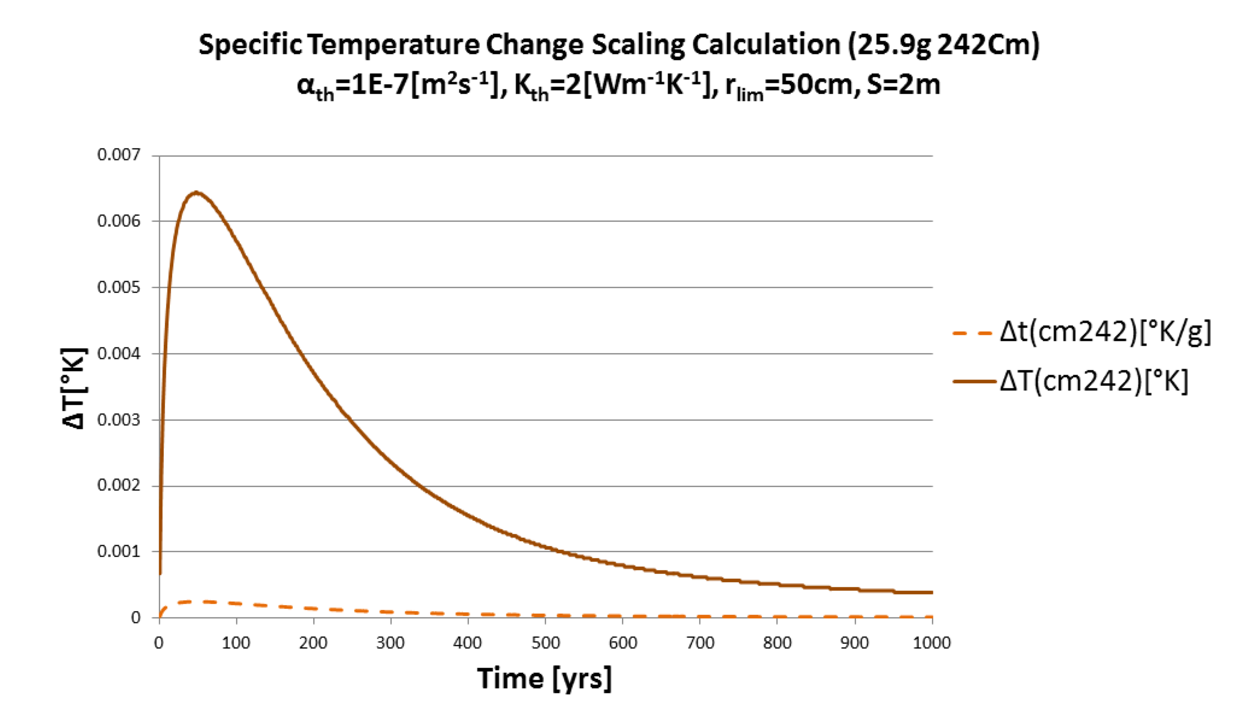
\includegraphics[width=\linewidth]{./images/CmScaling.eps}
\end{center}
\caption{As a demonstration of the calculation procedure, the temperature change 
  curve for one initial gram of $^{242}Cm$ and is scaled to represent $25.9g$, 
  approximately the $^{242}Cm$ inventory per MTHM in 51GWd burnup UOX PWR fuel. }
\label{fig:CmScaling}
\end{figure}
}
\end{frame}

\begin{frame}
\frametitle{Superposition Concept}
\footnotesize{

The supporting database was limited to some primary heat contributing isotopes 
present in traditional spent nuclear fuel, $H$, 
such that the superposition in equation \eqref{superposition} becomes 
\begin{align}
\Delta T (r_{lim},S,K_{th},\alpha_{th})&\sim \sum_{i\in H} m_i \Delta t_i(r_{lim},S,K_{th},\alpha_{th})
\label{superposition_approx}
\intertext{where}
H &= \mbox{ set of high heat isotopes }[-]\nonumber\\
S &= \mbox{ uniform waste package spacing } [m]\nonumber\\
K_{th} &= \mbox{ thermal conductivity } [W\cdot m^{-1}\cdot K^{-1}]\nonumber\\
\alpha_{th} &= \mbox{ thermal diffusivity } [m^2\cdot s^{-1}]\nonumber\\
\end{align}
}
\end{frame}


\begin{frame}
\frametitle{Superposition Demonstration}
\footnotesize{

\begin{figure}[ht!]
\begin{center}
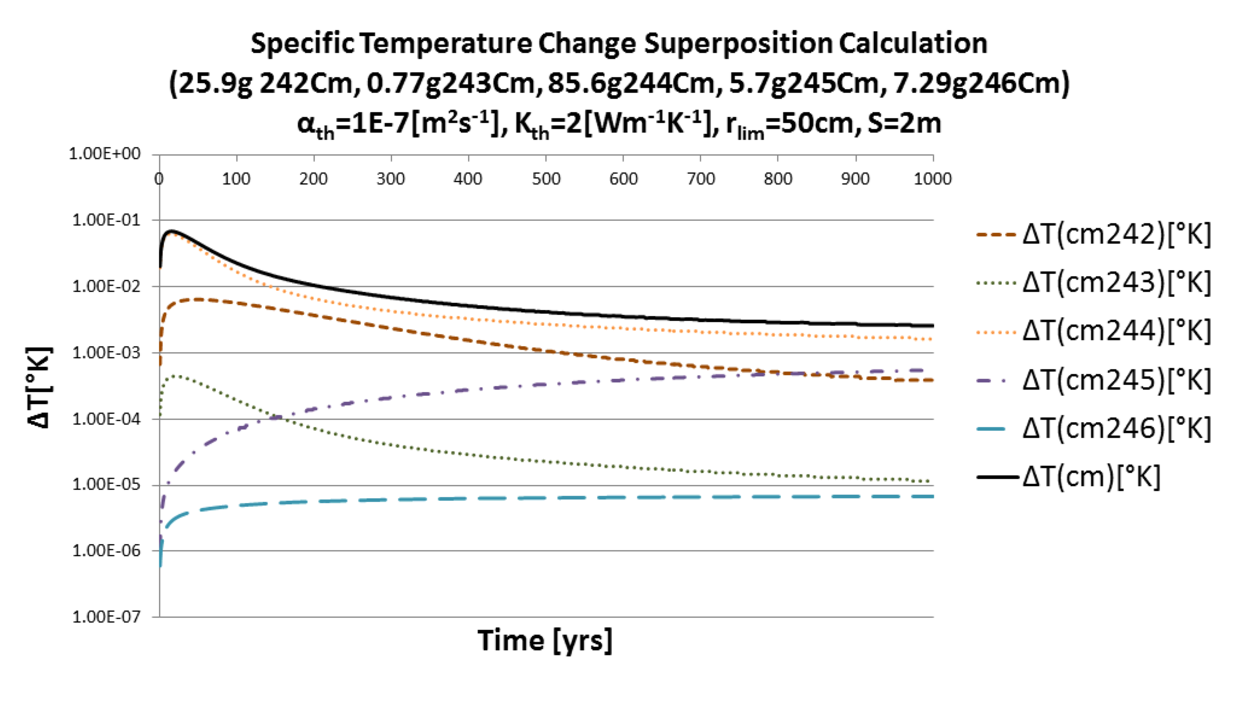
\includegraphics[width=\columnwidth]{./images/CmSuperposition.eps}
\end{center}
\caption{As a demonstration of the calculation procedure, scaled temperature change 
  curves for five curium isotopes are superimposed to achieve a total temperature 
change (note log scale).}
\label{fig:CmSuperposition}
\end{figure}

}
\end{frame}




\subsection{Radionuclide Transport in Cyder}

\begin{frame}
  \frametitle{Nested Components}
  The NuclideModel in a Component can be interchangeably represented by any of 
  the four nuclide transport models. 
    \begin{itemize}
      \item Degradation Rate Based Failure Model
      \item Mixed Cell with Degradation, Sorption, Solubility Limitation
      \item Lumped Parameter Model
      \item 1D van Genuchten Advection Dispersion Solution
    \end{itemize}
\end{frame}

\begin{frame}
  \frametitle{Advection Dispersion Equation}
  \footnotesize{
    In a saturated, reducing environment, contaminants are transported by 
    \textbf{dispersion} and \textbf{advection} 
    \cite{schwartz_fundamentals_2004, 
    wang_introduction_1982, van_genuchten_analytical_1982}: 
    \begin{align}
      J &= J_{dis} + J_{adv}\nonumber\\
      &= -\theta(D_{mdis} + \tau D_m)\nabla C + \theta vC\nonumber\\ 
      &= -\theta D\nabla C + \theta vC \nonumber\\ 
      \label{unidirflow}
      \intertext{where}
      J_{dis} &= \mbox{ Total Dispersive Mass Flux }[kg/m^2/s]\nonumber\\
      J_{adv} &= \mbox{ Advective Mass Flux }[kg/m^2/s]\nonumber\\
      \tau &= \mbox{ Toruosity }[-] \nonumber\\
      \theta &= \mbox{ Porosity }[-] \nonumber\\
      D_m &= \mbox{ Molecular diffusion coefficient }[m^2/s]\nonumber\\
      D_{mdis} &= \mbox{ Coefficient of mechanical dispersivity}[m^2/s]\nonumber\\
      D &= \mbox{ Effective Dispersion Coefficient }[m^2/s]\nonumber\\
      C &= \mbox{ Concentration }[kg/m^3]\nonumber\\
      v &= \mbox{ Fluid Velocity in the medium }[m/s].\nonumber
    \end{align}
    }

\end{frame}

\begin{frame}
  \frametitle{Component Interfaces}
  \footnotesize{
Solutions to this equation can be categorized by their boundary conditions and 
those boundary conditions serve as the interfaces between components in the 
Cyder library of nuclide transport models.

  \begin{figure}[htp!]
    \begin{center}
      \def\svgwidth{\textwidth}
      \input{images/flow.eps_tex}
    \end{center}
    \caption{The boundaries between components are robust interfaces defined by 
    Source Term, Dirichlet, Neumann, and Cauchy boundary conditions.}
    \label{fig:flow}
  \end{figure}
  }
\end{frame}

\begin{frame}
\frametitle{Implicit Timestepping}
\footnotesize{Each Component passes some information radially outward to the nested 
Component immediately containing it and some information radially 
inward to the nested Component it contains. 

Mass distribution in Component 0 at time $t_n$ is found from the inner boundary 
condition at time $t_n$ and the outer boundary condition at $t_{n-1}$. Outer 
boundary conditions are solved for numerically at $t_n$.
For each timestep :

\begin{align}
  BC(i, r_o, c_1, t_n) &= f( BC(i, r_i, c_0, t_n), BC(i, r_o, c_1, t_{n-1}) )
  \intertext{where}
  BC  &= \mbox{boundary condition }\nonumber\\
  i &= \mbox{the isotope }\nonumber\\
  r_i &= \mbox{the inner boundary radius } [m]\nonumber\\
  r_o &= \mbox{the outer boundary radius } [m]\nonumber\\
  c_0 &= \mbox{the innermost Component}\nonumber\\
  c_1 &= \mbox{the Component that contains c}_0\nonumber\\
  f &= \mbox{functional form of the contaminant transport algorithm}\nonumber\\
  t_n &= \mbox{timestep n.}\nonumber
\end{align}
}
\end{frame}

\begin{frame}
\frametitle{Clay GDSM Model.}
explain
\end{frame}

\begin{frame}
  \frametitle{Radionuclide Transport: Degradation Rate Based Release}
  \footnotesize{
In this model, the contaminants in the degraded fraction of the control volume 
are available to adjacent components. The available contaminants
$m_{ij}(t)$, at the boundary between cell $i$ to cell $j$ at time $t$ are thus

\begin{align}
\dot{m}_{ij}(t) &= f_im_i(t)
\label{deg_rate_source_cont}
\intertext{where}
\dot{m}_{ij} &= \mbox{ the rate of mass transfer from i to j }[kg/s]\nonumber\\
f_i &= \mbox{ degradation rate function in cell i }[1/s] \nonumber\\
m_i &= \mbox{ mass in cell i }[kg] \nonumber\\
t &= \mbox{ time  }[s].\nonumber
\end{align}
}
\end{frame}


\begin{frame}
  \frametitle{Radionuclide Transport: Degradation Rate Based Release}
  \begin{figure}[h!]
  \begin{center}
    \def\svgwidth{.7\textwidth}
    \begin{figure}[h!]
  \begin{center}
    \def\svgwidth{.7\textwidth}
    \input{./images/deg_volumes.eps_tex}
  \end{center}
  \caption[Constituents of a Degradation Rate Control Volume]{The control volume contains an 
  intact volume $V_i$ and a degraded volume, $V_d$. Contaminants in $V_d$ are 
  available for transport, while contaminants in $V_i$ are contained.}
  \label{fig:deg_volumes}
\end{figure}


  \end{center}
  \caption[Constituents of a Degradation Rate Control Volume]{The control volume contains an 
  intact volume $V_i$ and a degraded volume, $V_d$. Contaminants in $V_d$ are 
  available for transport, while contaminants in $V_i$ are contained.}
  \label{fig:deg_volumes}
\end{figure}


\end{frame}

\begin{frame}
  \frametitle{Radionuclide Transport : Mixed Cell with Sorption and Solubility}
  \begin{figure}[h!]
  \begin{center}
    \def\svgwidth{\textwidth}
    \begin{figure}[h!]
  \begin{center}
    \def\svgwidth{\textwidth}
    \input{./images/deg_sorb_volumes.eps_tex}
  \end{center}
  \caption[Constituents of a Mixed Cell Control Volume]{The degraded volume is 
  modeled as a solid degraded volume, $V_{ds}$, and a fluid degraded volume, 
  $V_{df}$. The intact volume is modeled as an intact solid volume, $V_{is}$, and 
  an intact fluid volume $V_{if}$.  Only contaminants in $V_{df}$ are available 
  for transport.}
  \label{fig:deg_sorb_volumes}
\end{figure}


  \end{center}
  \caption[Constituents of a Mixed Cell Control Volume]{The degraded volume is 
  modeled as a solid degraded volume, $V_{ds}$, and a fluid degraded volume, 
  $V_{df}$. The intact volume is modeled as an intact solid volume, $V_{is}$, and 
  an intact fluid volume $V_{if}$.  Only contaminants in $V_{df}$ are available 
  for transport.}
  \label{fig:deg_sorb_volumes}
\end{figure}


\end{frame}

\begin{frame}
  \frametitle{Radionuclide Transport : Mixed Cell Sorption}
The mass of contaminant sorbed into the degraded and precipitated solids can be
found using a linear isotherm model \cite{schwartz_fundamentals_2004},
characterized by the relationship 
\begin{align}
s_{i} &= K_{di} C_{i}
\label{linear_iso}
\intertext{where}
s_i &= \mbox{ the solid concentration of isotope i }[kg/kg]\nonumber\\
K_{di} &= \mbox{ the distribution coefficient of isotope i}[m^3/kg]\nonumber\\
C_i &= \mbox{ the liquid concentration of isotope i }[kg/m^3].\nonumber
\end{align}
\end{frame}

\begin{frame}
  \frametitle{Radionuclide Transport : Mixed Cell Solubility Limitation}
  \footnotesize{
In addition to engineered barriers, contaminant transport is constrained by 
  the solubility limit \cite{hedin_integrated_2002}, 
    \begin{align}
      m_{s,i} &\leq V_w C_{sol,i},
    \intertext{where}
      m_{s,i} &= \mbox{ solubility limited mass of isotope i in volume }V_w [kg]\nonumber\\ 
      V_w &= \mbox{ volume of the solution }[m^3]\nonumber\\
      C_{sol,i} &= \mbox{ solubility limit, the maximum concentration of i }[kg/m^3].\nonumber
    \end{align}


The desired boundary conditions can be expressed in terms of $m_{ffl}$. First, the 
Dirichlet boundary condition is 
\begin{align}
C(x,y,z,t) = \frac{m_{ffl}(t)}{V_{ff}(t)}\forall (x,y,x) \in \Gamma.
\label{dirichlet_mixed}
\end{align}

From this boundary condition in combination with global advective velocity 
data, all other boundary conditions can be found. 
    }
\end{frame}

\begin{frame}
  \frametitle{Radionuclide Transport: Lumped Parameter Transport Model}
\footnotesize{
\begin{figure}[htbp!]
  \begin{center}
    \def\svgwidth{\textwidth}
    \input{images/lumpedseries.eps_tex}
  \end{center}
  \caption{ The method by which each lumped parameter component is modeled is
according to a relationship between the incoming concentration, $C_{in}(t)$,
and the outgoing concentration, $C_{out}(t)$.}
  \label{fig:lumpedseries}
\end{figure}

\begin{align}
  C_{out}(t) &= \int_0^\infty C_{in}(t-t')g(t')e^{-\lambda t'}dt'
  \label{lumped2}
  \intertext{where}
  t'  &= \mbox{ time of entry }[s]\nonumber\\
  t-t'  &= \mbox{ transit time }[s]\nonumber\\
  g(t-t')  &= \mbox{ response function, a.k.a. transit time distribution}[-]\nonumber\\
  \lambda &= \mbox{ radioactive decay constant}[s^{-1}].\nonumber
\end{align}
}
\end{frame}

\begin{frame}
  \frametitle{Radionuclide Transport: Lumped Parameter Transport Model}
\footnotesize{
Selection of the response function is usually based on experimental tracer
results in the medium at hand. However, some functions used commonly in
chemical engineering applications \cite{maloszewski_lumped_1996} include the
Piston Flow Model (PFM), 
\begin{align}
  g_{PFM}(t') &= \delta{(t'-t_t))}
  \intertext{ the Exponential Model (EM) }
  g_{EM}(t') &= \frac{1}{t_t}e^{-\frac{t'}{t_t}}
  \intertext{ and the Dispersion Model (DM), }
  g_{DM}(t') &= \left( \frac{\text{Pe }t_t}{4\pi t'} \right)^{\frac{1}{2}}
  \frac{1}{t'}e^{- \frac{\text{Pe }t_t\left( 1- \frac{t'}{t_t}  \right)^2} 
  {4t'}}, \intertext{where}
  \text{Pe}  &= \mbox{ Peclet number for mass diffusion }[-]\nonumber\\
  t_t  &= \mbox{ mean tracer age }[s]\nonumber\\
    &= t_w \mbox{ if there are no stagnant areas }\nonumber\\
  t_w  &= \mbox{ mean residence time of water }[s]\nonumber\\
       &= \frac{V_m}{Q}\nonumber\\
       &= \frac{z}{v_z}\nonumber\\
       &= \frac{z\theta_e}{q}\nonumber
  \intertext{in which}
  V_m  &= \mbox{ mobile water volume }[m^3]\nonumber\\
  Q    &= \mbox{ volumetric flow rate }[m^3/s]\nonumber\\
  z    &= \mbox{ average travel distance in flow direction }[m]\nonumber\\
  v_z  &= \mbox{ mean water velocity}[m/s]\nonumber\\
  q    &= \mbox{ Darcy Flux }[m/s]\nonumber\\
  \theta_e &= \mbox{ effective (connected) porosity }[\%].\nonumber
\end{align}
}
\end{frame}

\begin{frame}
  \frametitle{Radionuclide Transport: Lumped Parameter Transport Model}
\footnotesize{
The solutions to these for constant concentration at the 
source boundary are given in \cite{maloszewski_lumped_1996}, 
\begin{align}
  C(t) &=\begin{cases}
    PFM & C_0e^{-\lambda t_t}\\
    EM  & \frac{C_0}{1+\lambda t_t}\\
    DM & C_0e^{\frac{\texttt{Pe}}{2}\left(1-\sqrt{1+\frac{4\lambda 
    t_t}{\texttt{Pe}}}\right)}.
  \end{cases}
  \label{lumpedsolns}
\end{align}
}
\end{frame}


\begin{frame}
  \frametitle{Radionuclide Transport: 1D Finite, Cauchy B.C.}
  \footnotesize{
\begin{figure}[htbp!]
  \begin{center}
    \def\svgwidth{.5\textwidth}
    \input{images/1dfin.eps_tex}
  \end{center}
  \caption{A one dimensional, finite, unidirectional flow,
  solution with Cauchy and Neumann boundary conditions}
  \label{fig:1dinf}
\end{figure}
}
\end{frame}

\begin{frame}
  \frametitle{Radionuclide Transport: 1D Finite, Cauchy B.C.}
For the boundary conditions, 
\begin{align}
  -D \frac{\partial C}{\partial z}\big|_{z=0} + v_zc &= \begin{cases}
    v_zC_0  &  \left( 0<t<t_0 \right)\\
    0  &  \left( t>t_0 \right)\\
  \end{cases}
\intertext{and}
  \frac{\partial C}{\partial z}\big|_{z=L} &= 0
  \intertext{and the initial condition,}
  C(z,0) &= C_i,
  \label{1dinfBC}
  \intertext{the solution is given as }
  C(z,t) &= \begin{cases} 
  C_i + \left(C_0 - C_i\right)A\left(z,t\right) & 0<t\le t_0\\
  C_i + \left(C_0 - C_i\right)A\left(z,t\right) - C_0A(z,t-t_0) & t\ge t_0.
  \end{cases}
\end{align}
\end{frame}

\begin{frame}
  \frametitle{Radionuclide Transport: 1D Finite, Cauchy B.C.}
\footnotesize{For the vertical flow coordinate system, $A$ is defined as
\begin{align}
A(z,t) =& \left(\frac{1}{2}\right)\erfc{\left[\frac{Rz-vt}{2\sqrt{DRt}}\right]} \nonumber\\
&+ \left(\frac{v^2t}{\pi RD}\right)^{1/2}\exp{\left[-\frac{(Rz-vt)^2}{4DRt}\right]}\nonumber\\ 
&- \frac{1}{2} \left(1+\frac{vz}{D} + \frac{v^2t}{DR}\right) \exp{\left[\frac{vz}{D}\right]}\erfc{\left[\frac{Rz+vt}{2\sqrt{DRt}}\right]}\nonumber\\
&+ \left(\frac{4v^2t}{\pi RD}\right)^{1/2}\left[1+\frac{v}{4D}\left(2L-z+\frac{vt}{R}\right)\right]\exp{\left[\frac{vL}{D} - \frac{R}{4Dt}\left(2L-z+\frac{vt}{R}\right)^2\right]}\nonumber\\
&- \frac{v}{D}\left[2L - z + \frac{3vt}{2R} + \frac{v}{4D}\left(2L - z + \frac{vt}{R}\right)^2\right]\exp{\left[\frac{vL}{D}\right]}\erfc{\left[\frac{R(2L-z) + vt}{2\sqrt{DRt}}\right]}\nonumber
\intertext{where}
L =& \mbox{Extent of the solution domain }[m]\nonumber\\
R =& \mbox{Retardation factor }[-].\nonumber
\end{align}
}
\end{frame}


\section{Demonstration}


\begin{frame}[ctb!]
  \frametitle{lp}
  
\begin{frame}[ctb!]
\begin{figure}[ht]
\centering
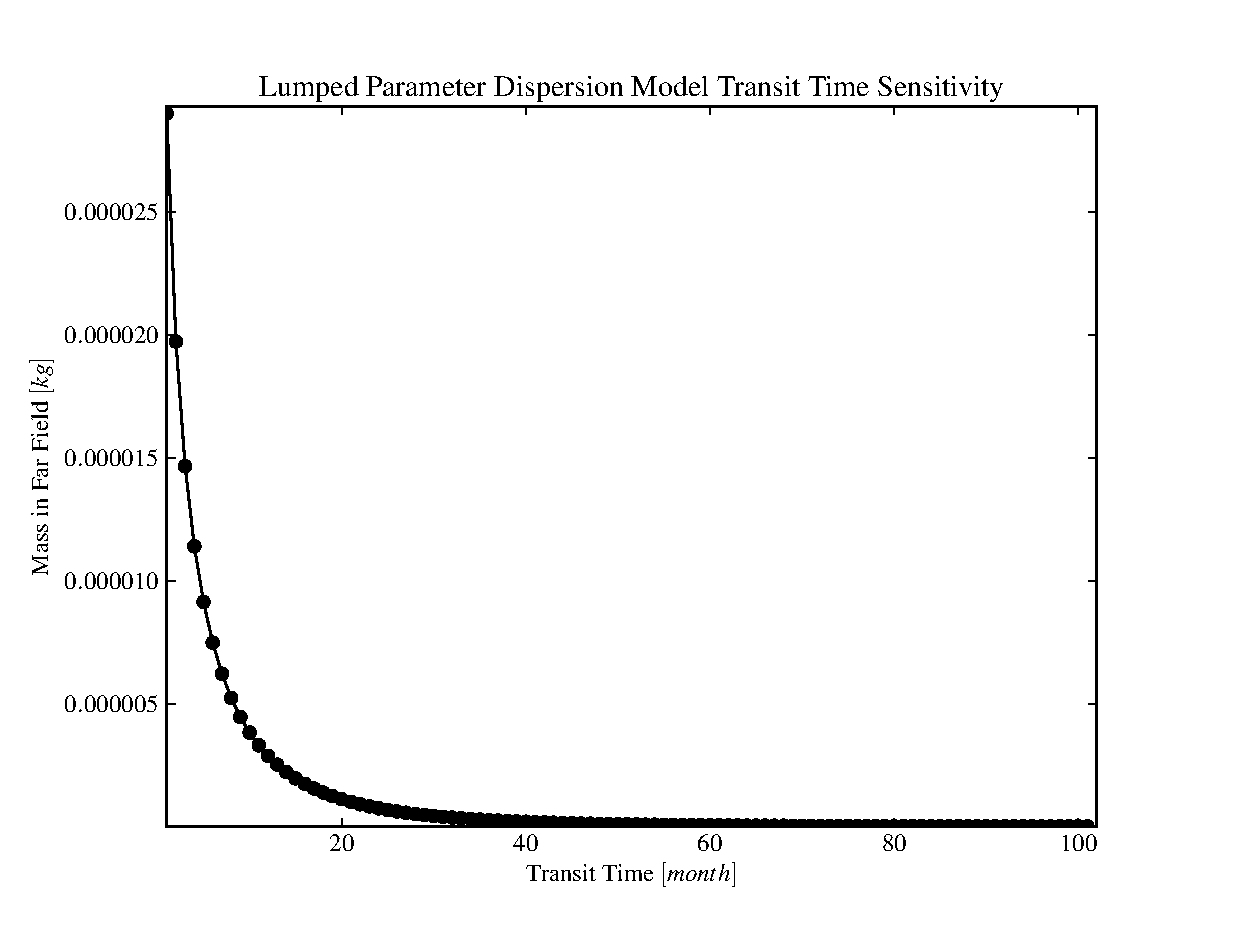
\includegraphics[width=0.8\textwidth]{./chapters/demonstration/base/lpDM_t_t.eps}
\caption[Lumped Parameter Dispersion Model Transit Time Sensitivity]{The transit time 
parameterization of the lumped parameter dispersion model of radionuclide 
transport has a strong effect on the material reaching the far field after 30 
years.  }
\label{fig:lp_t_t_begin}
\end{figure}
\end{frame}

\begin{frame}[ctb!]
\begin{figure}[ht]
\centering
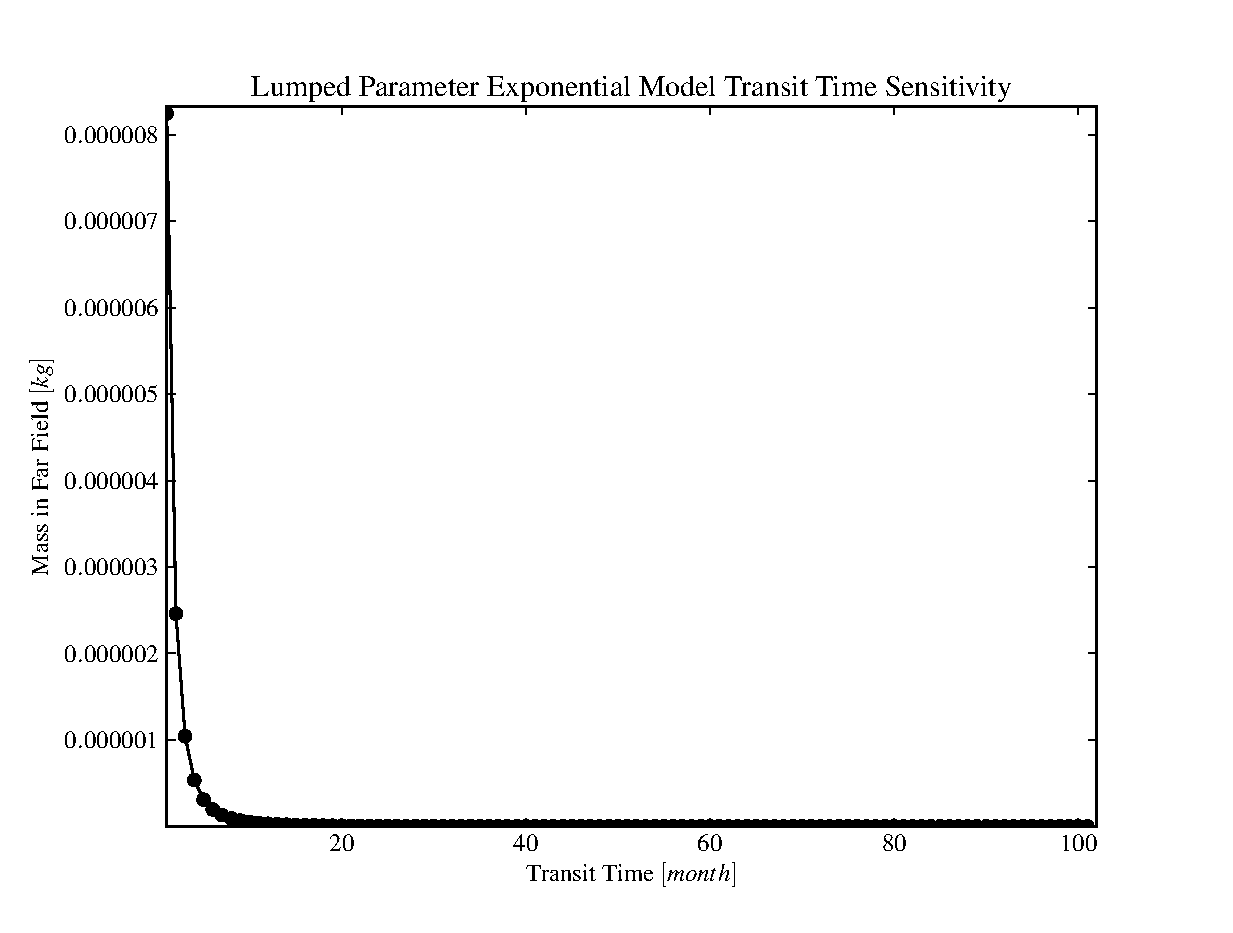
\includegraphics[width=0.8\textwidth]{./chapters/demonstration/base/lpEXPM_t_t.eps}
\caption[Lumped Parameter Exponential Model Transit Time Sensitivity]{The transit time 
parameterization of the lumped parameter exponential model of radionuclide 
transport has a strong effect on the material reaching the far field after 30 
years.  }
\end{figure}
\end{frame}

\begin{frame}[ctb!]
\begin{figure}[ht]
\centering
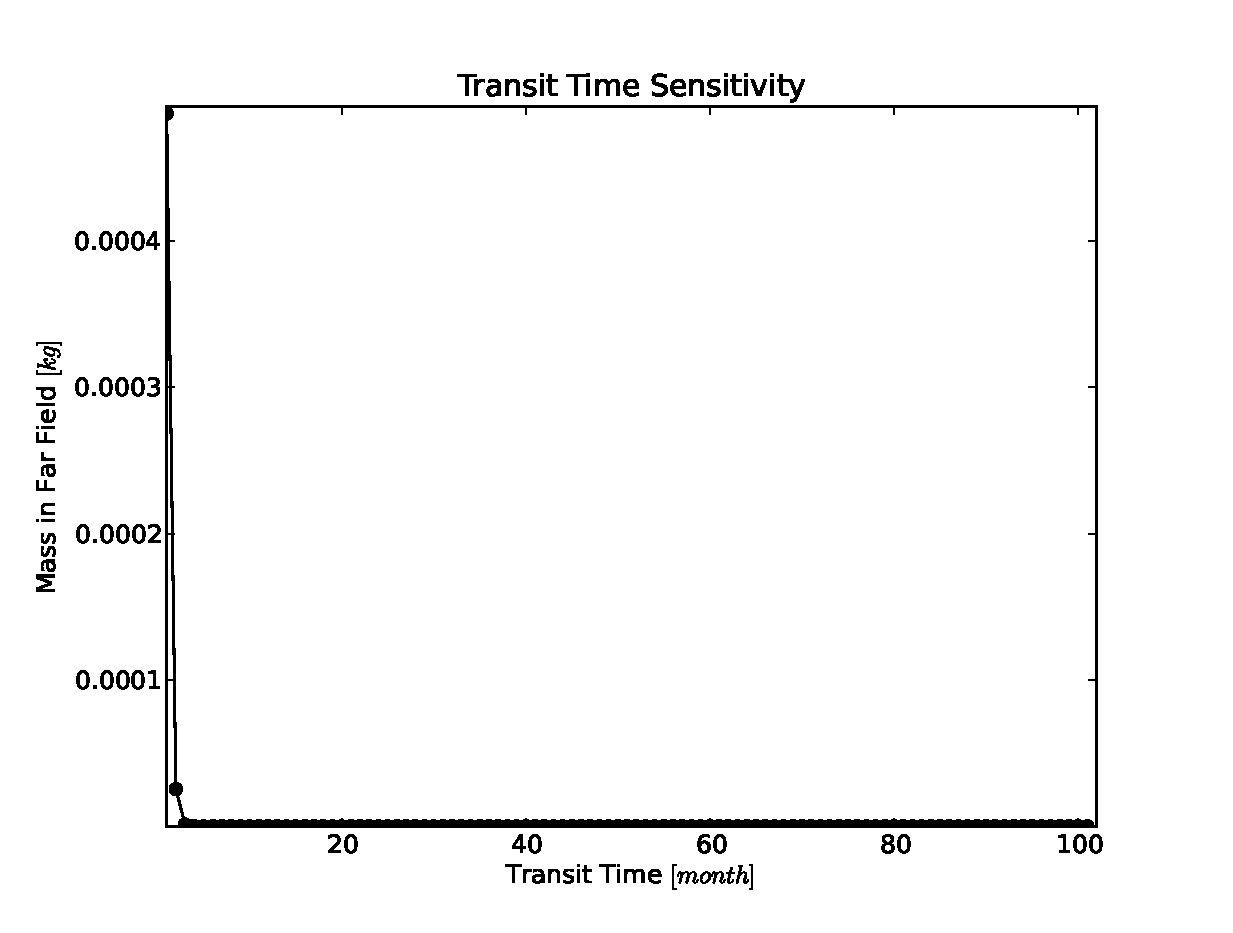
\includegraphics[width=0.8\textwidth]{./chapters/demonstration/base/lpPFM_t_t.eps}
\caption[Lumped Parameter Piston Flow Model Transit Time Sensitivity]{The transit time 
parameterization of the lumped parameter piston flow model of radionuclide 
transport has a strong effect on the material reaching the far field after 30 
years.  }
\label{fig:lp_t_t_end}
\end{figure}
\end{frame}

  \end{minipage}
\end{frame}

\subsection{Radionuclide Transport Toy Cases}


\begin{frame}[ctb!]
  \frametitle{Degradation Rate Model Base Case I}
\begin{figure}[ht]
\centering
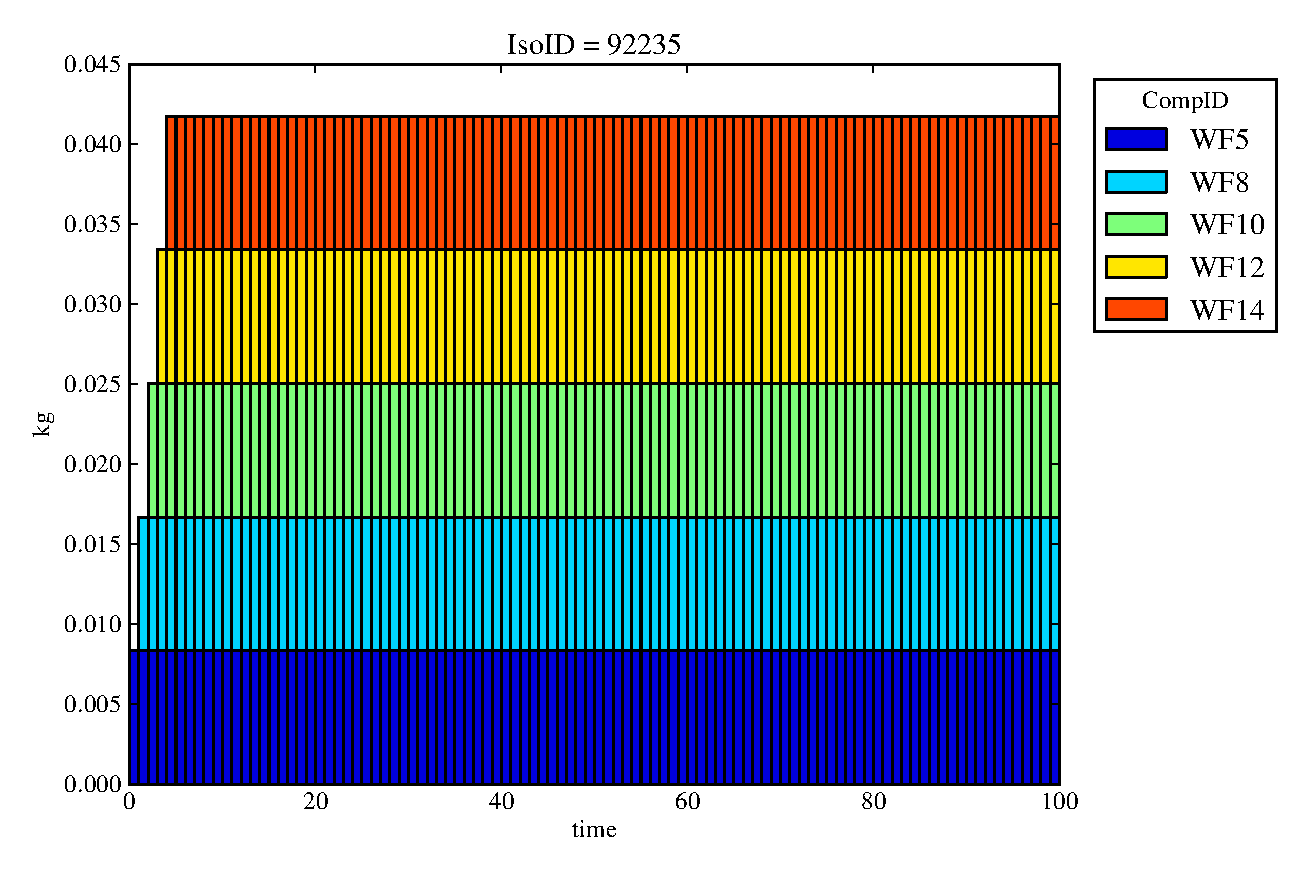
\includegraphics[width=0.8\textwidth]{./images/drI.eps}
\caption[$^{235}U$ residence. Degradation Rate Waste Form No Release.]{
For Case DRI, in which total containment in the waste form is assumed ($F_{d,wf}=0$), 
$^{235}U$ takes up permanent residence in the waste form component.
}
\label{fig:drIall}
\end{figure}
\end{frame}

\begin{frame}
  \frametitle{Degradation Rate Model Base Case I}
  \begin{figure}

\begin{minipage}[b]{0.45\linewidth}

  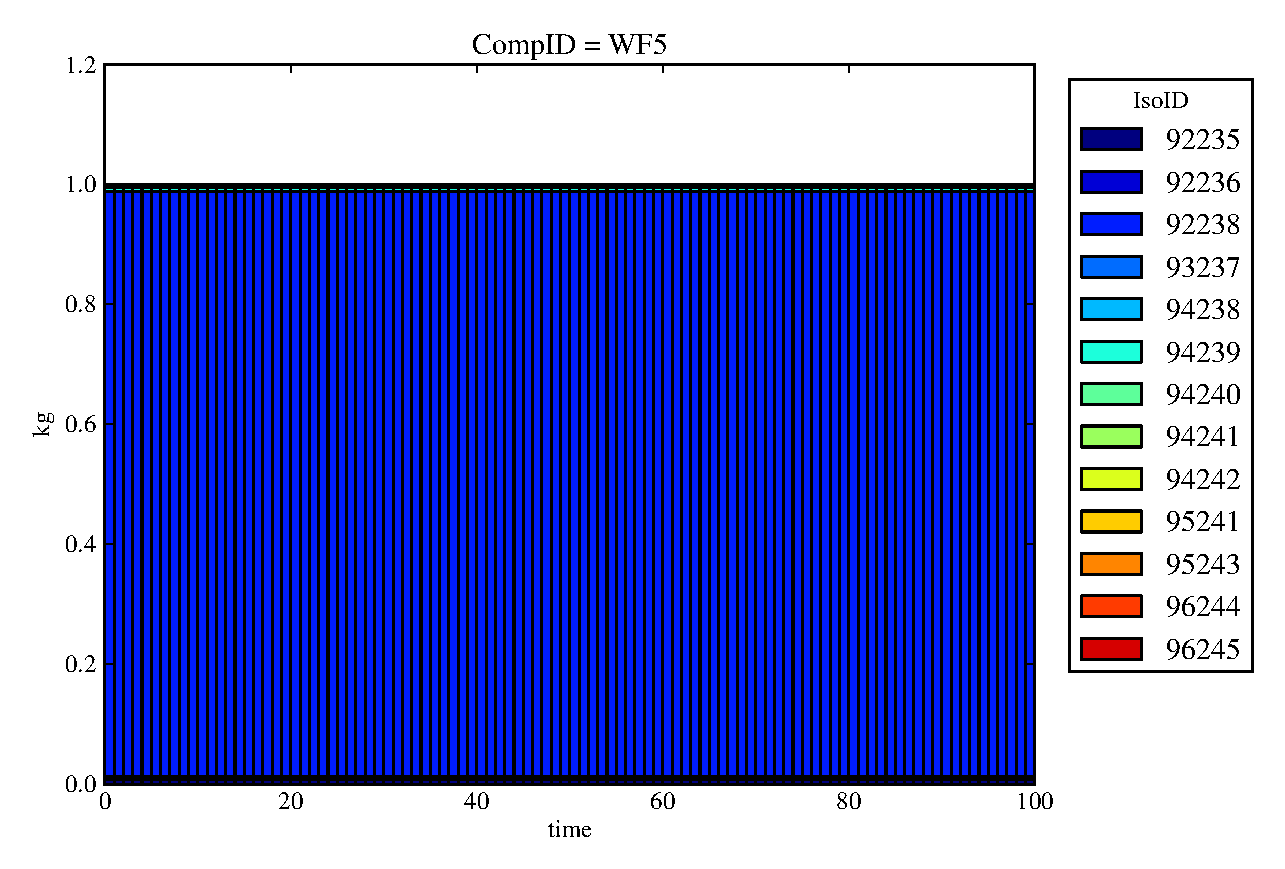
\includegraphics[width=0.8\textwidth]{./images/drI1.eps}
  \caption[DRI Waste Form Contaminants.]{
    Waste Form 5 ($F_d = 0$) never releases material.
    }
  \label{fig:drIwf5}
  
  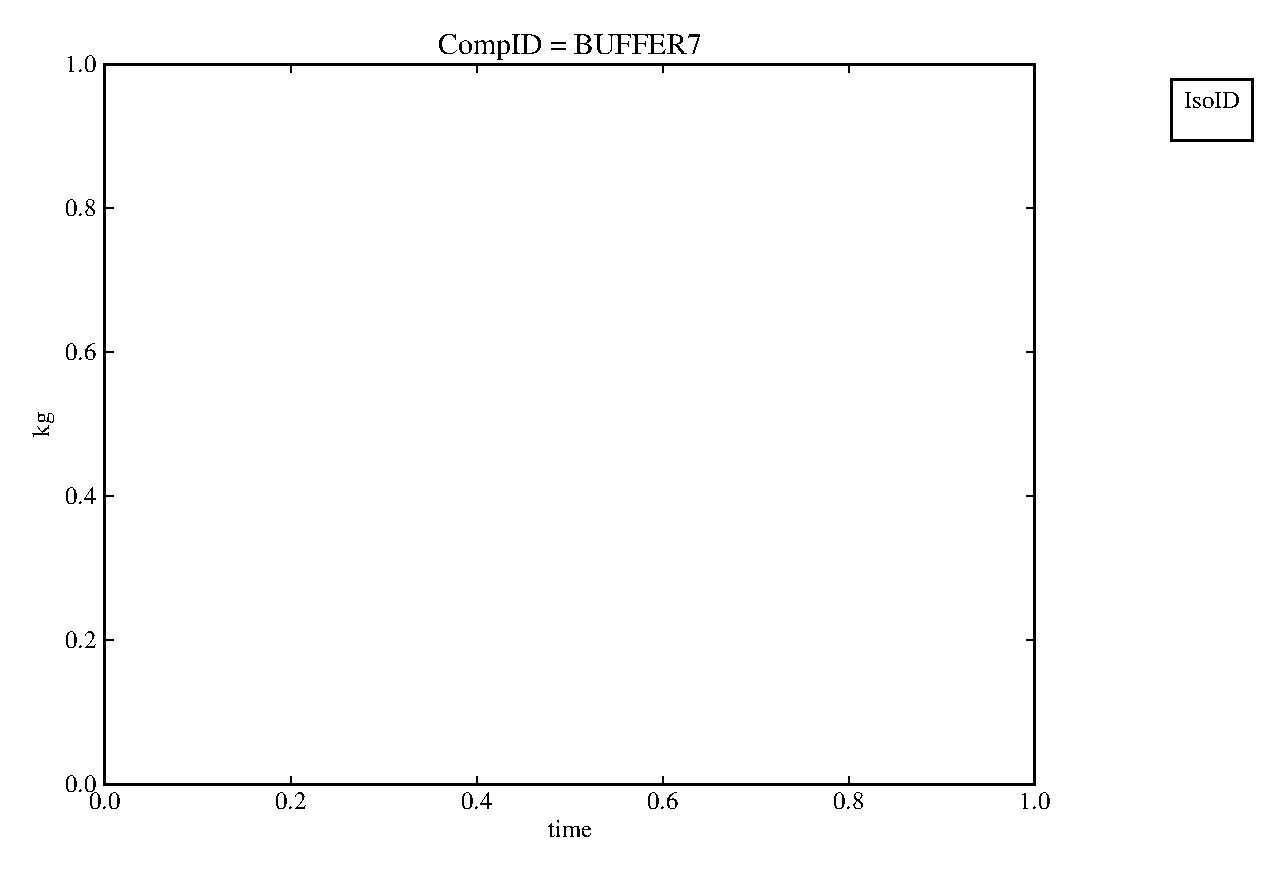
\includegraphics[width=0.8\textwidth]{./images/drI3.eps}
  \caption[Case DRI Buffer Contaminants]{
    The Buffer, component 7 ($F_d = 0.1$), never receives material.
    }
  \label{fig:drIbuff}

\end{minipage}
\hspace{0.05\linewidth}
\begin{minipage}[b]{0.45\linewidth}
  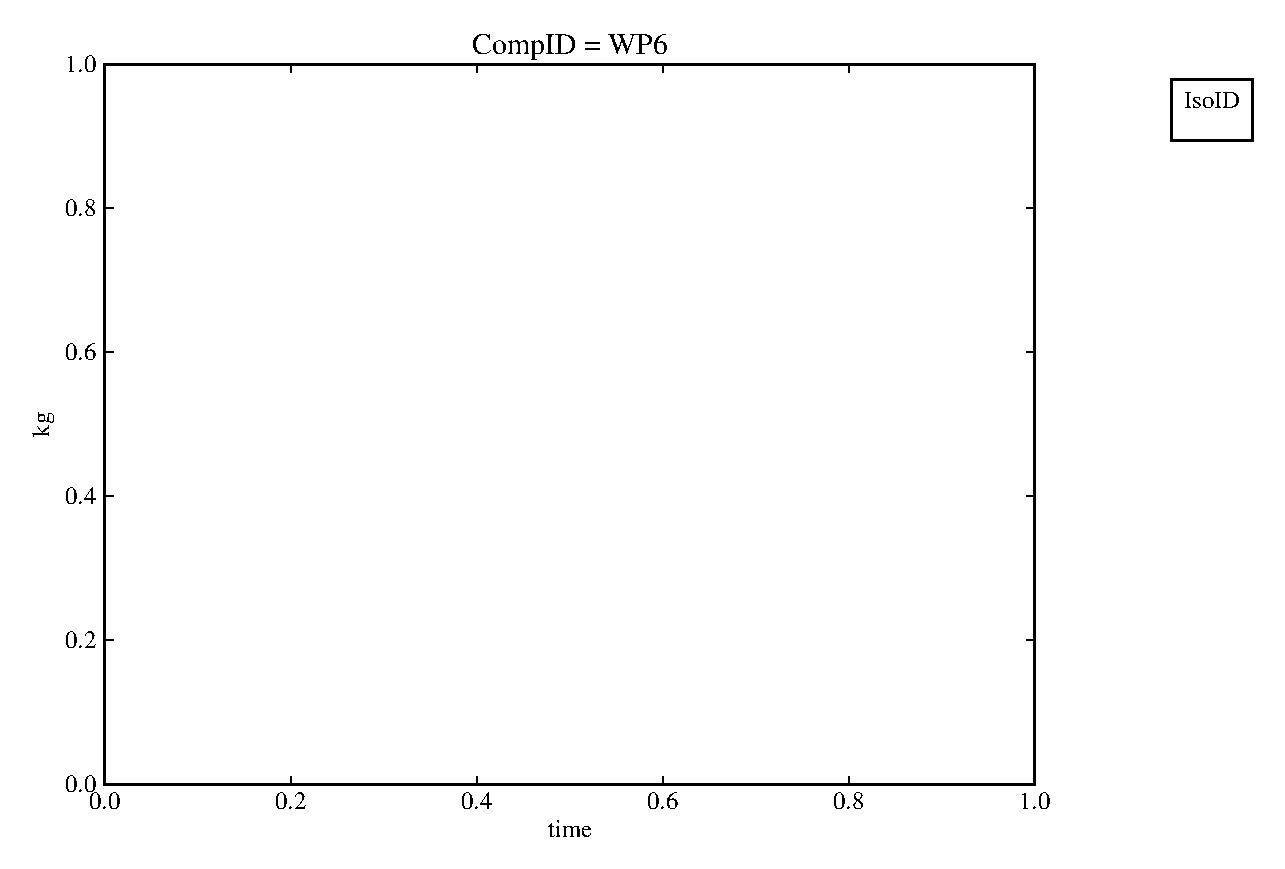
\includegraphics[width=0.8\textwidth]{./images/drI2.eps}
  \caption[Case DRI Waste Package Contaminants.]{ 
    Waste Package 6 ($F_d = 0.1$), never receives material.
    }
  \label{fig:drIwp6}

  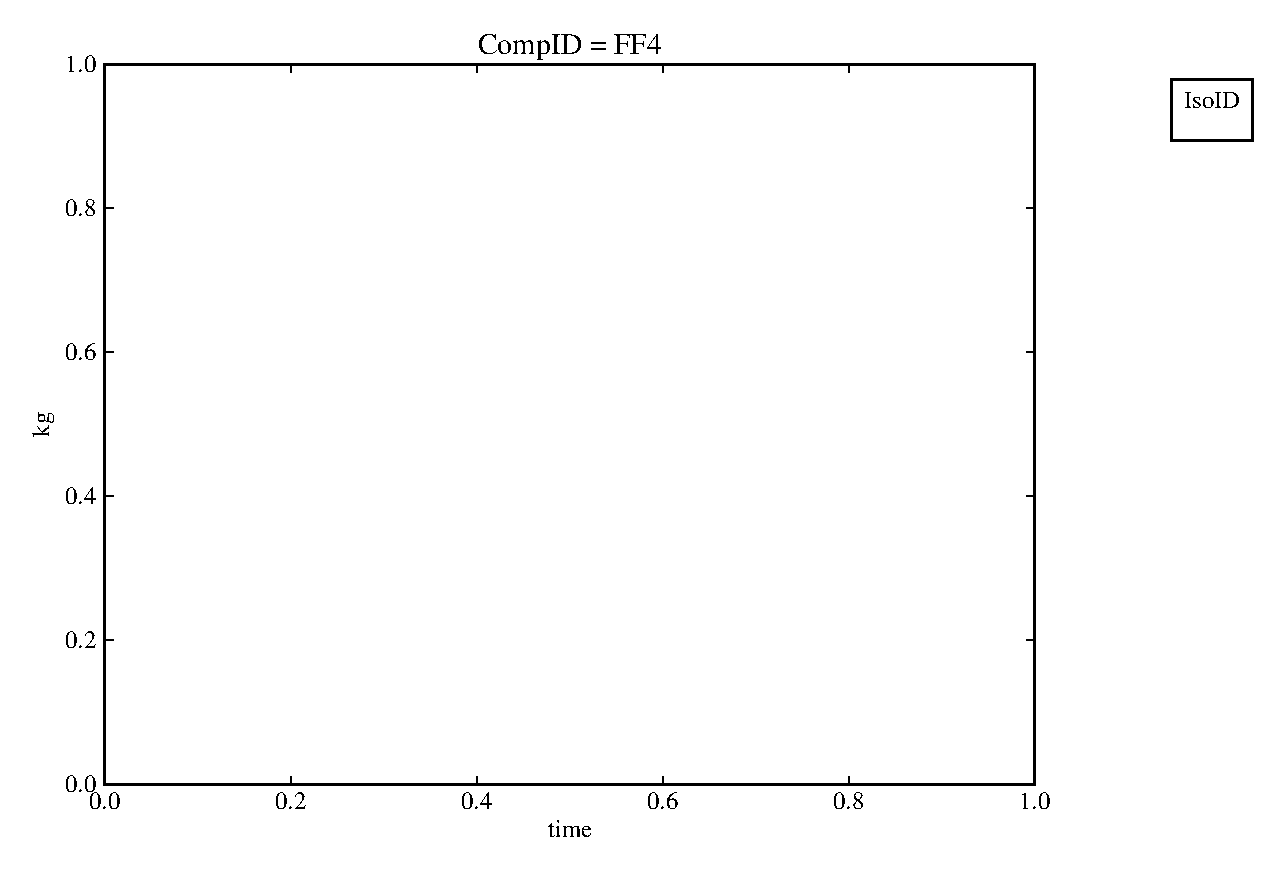
\includegraphics[width=0.8\textwidth]{./images/drI0.eps}
  \caption[Case DRI Far Field Contaminants.]{ 
    Far Field 4 ($F_d = 0.1$) never receives material.
    }
  \label{fig:drIff0}

  \end{minipage}
\end{figure}
\end{frame}



\begin{frame}[ctb!]
  \frametitle{Degradation Rate Model Base Case II}
\begin{figure}[ht]
\centering
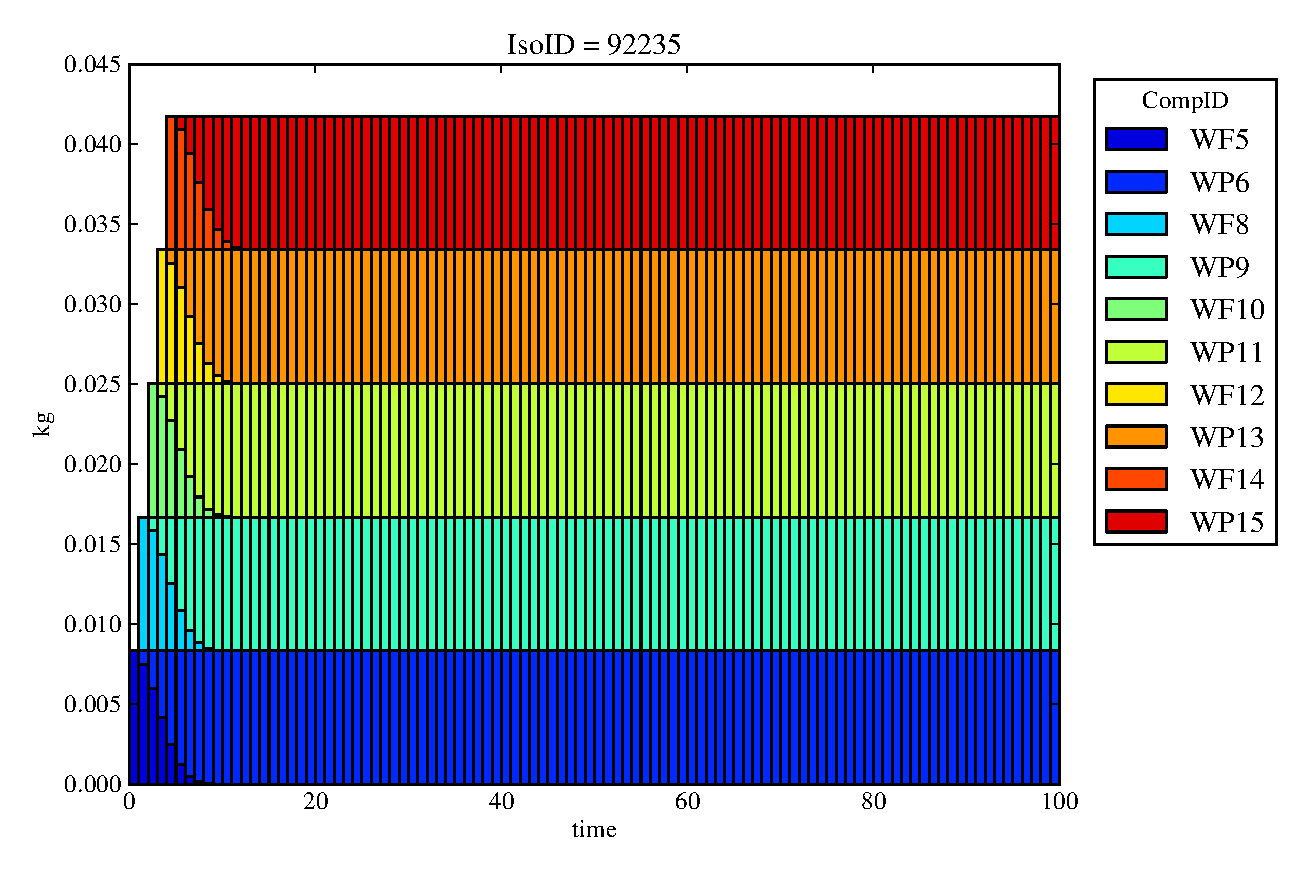
\includegraphics[width=0.8\textwidth]{./images/drII.eps}
\caption[$^{235}U$ residence. Degradation Rate Waste Package No Release.]{
For Case DRII, in which total containment in the waste package is assumed ($F_{d,wp}=0$), 
$^{235}U$ travels through waste forms ($F_d = 0.1$) before 
permanent residence in the waste package components.
}
\label{fig:drIIall}
\end{figure}
\end{frame}

\begin{frame}
  \frametitle{Degradation Rate Model Base Case II}
  \begin{figure}
\begin{minipage}[b]{0.45\linewidth}

  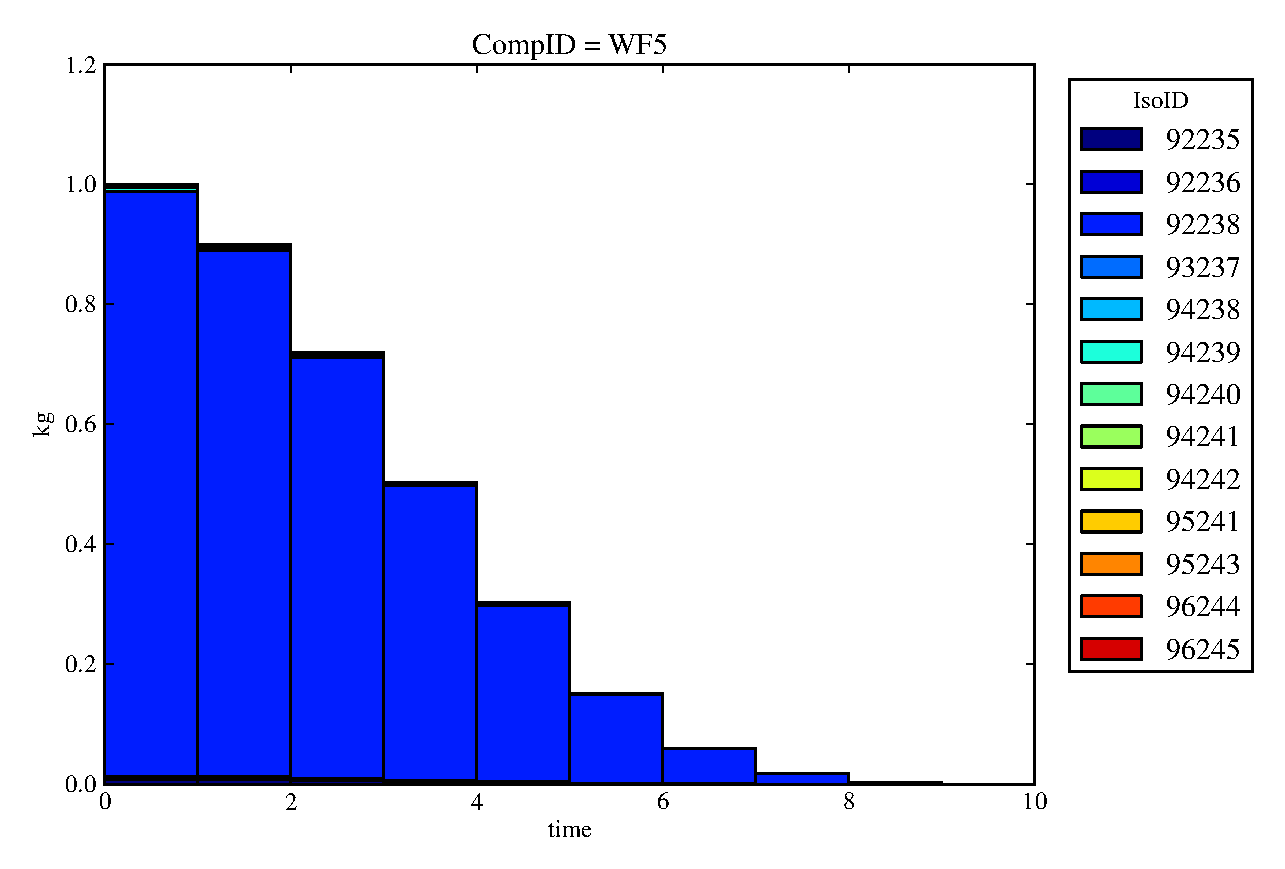
\includegraphics[width=0.8\textwidth]{./images/drII1.eps}
  \caption[DRII Waste Form Contaminants.]{
    Waste Form 5 ($F_d = 0.1$) releases material with degradation. 
    }
  \label{fig:drIIwf5}
  
  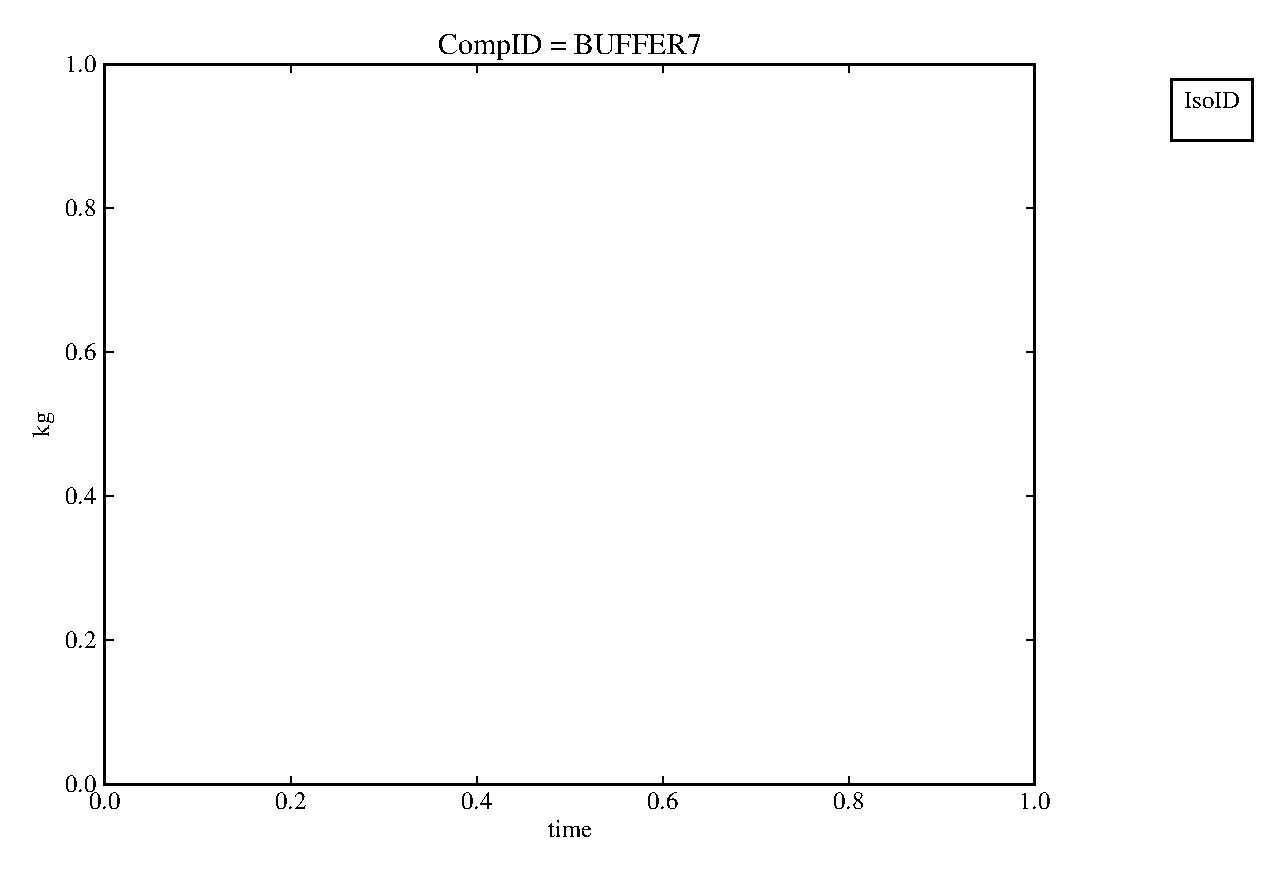
\includegraphics[width=0.8\textwidth]{./images/drII3.eps}
  \caption[Case DRII Buffer Contaminants]{
    The Buffer, component 7 ($F_d = 0.1$), never receives material.
    }
  \label{fig:drIIbuff}

\end{minipage}
\hspace{0.05\linewidth}
\begin{minipage}[b]{0.45\linewidth}
  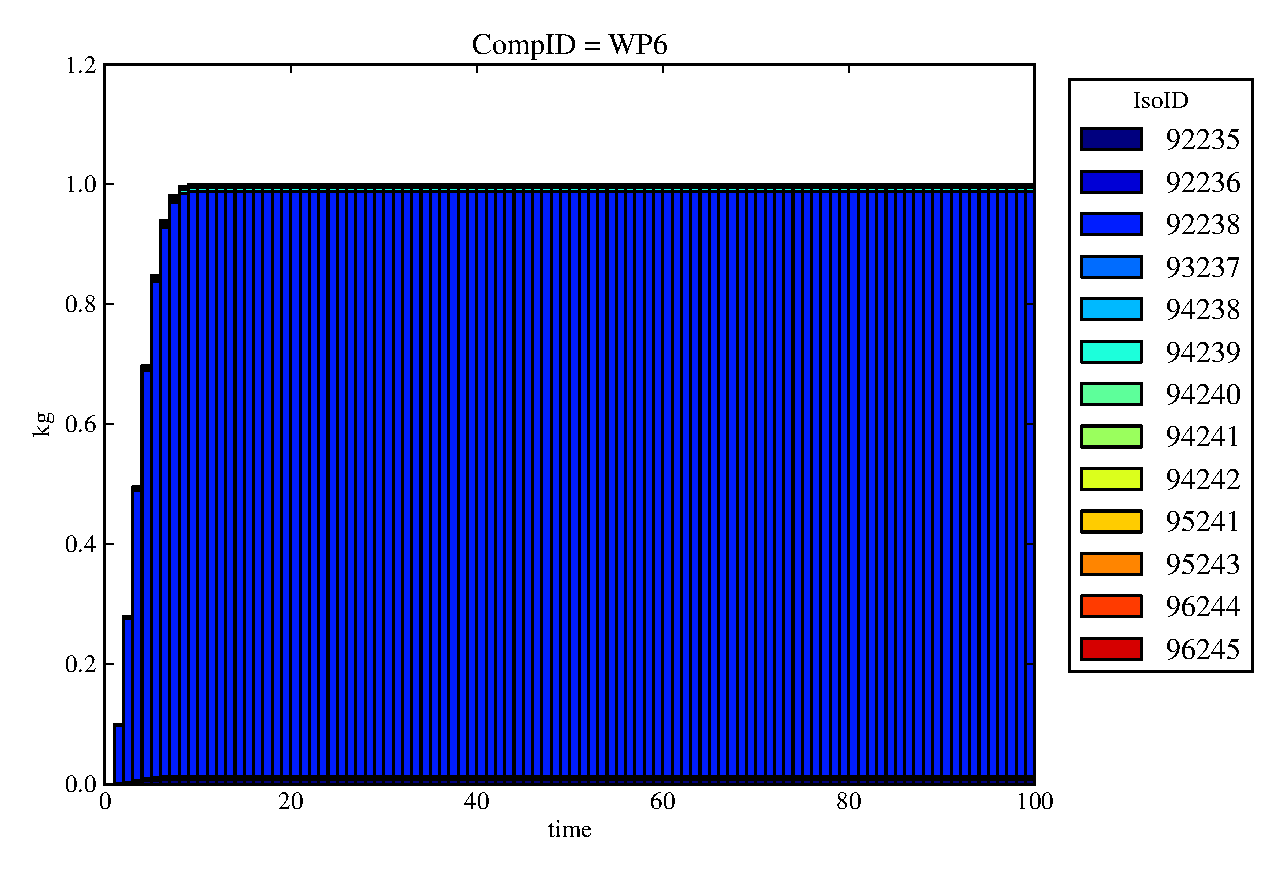
\includegraphics[width=0.8\textwidth]{./images/drII2.eps}
  \caption[Case DRII Waste Package Contaminants.]{ 
    Waste Package 6 ($F_d = 0$) acheives total containment.
    }
  \label{fig:drIIwp6}

  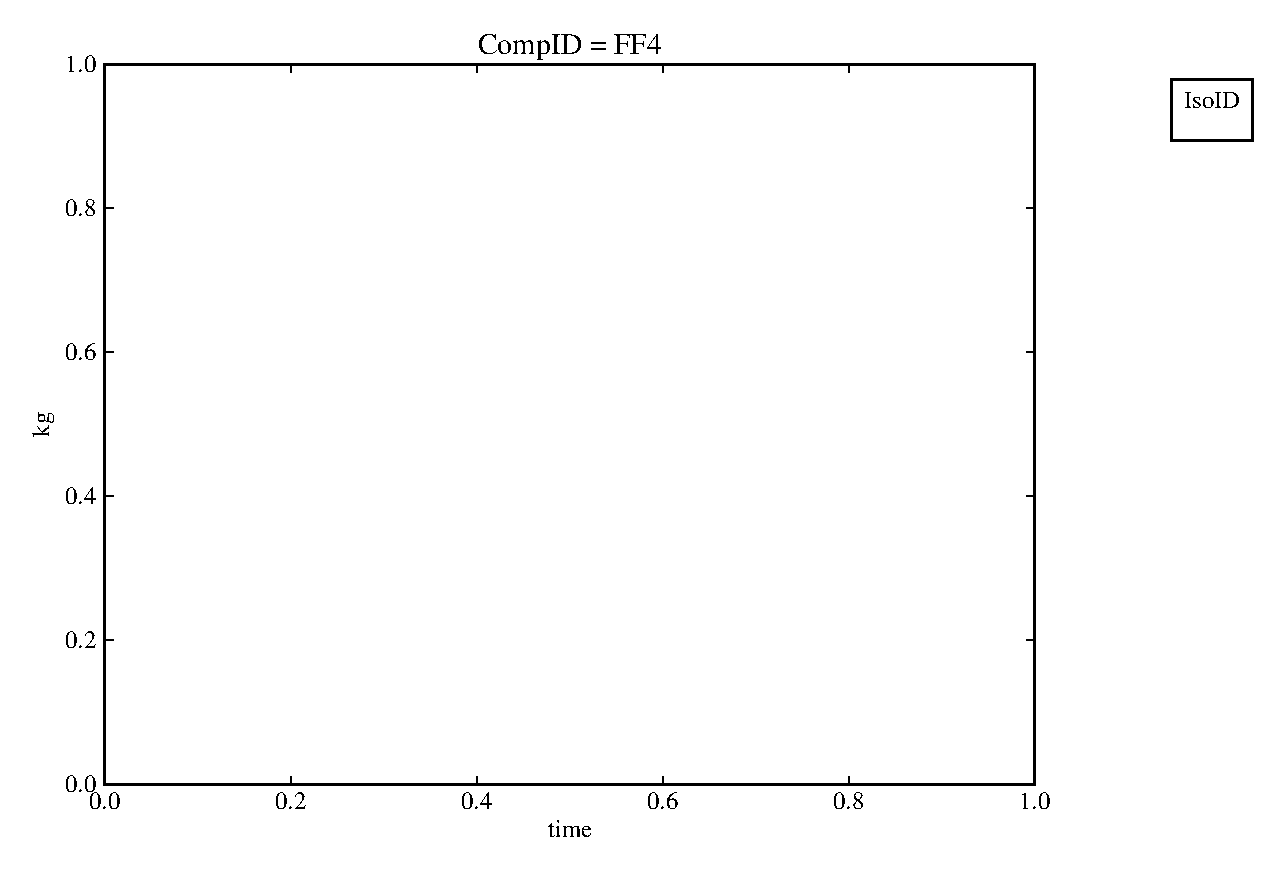
\includegraphics[width=0.8\textwidth]{./images/drII0.eps}
  \caption[Case DRII Far Field Contaminants.]{ 
    Far Field 4 ($F_d = 0.1$), never receives material.
    }
  \label{fig:drIIff0}


  \end{minipage}
\end{figure}
\end{frame}

\begin{frame}[ctb!]
\begin{figure}[ht]
  \frametitle{Degradation Rate Model Base Case III}
\centering
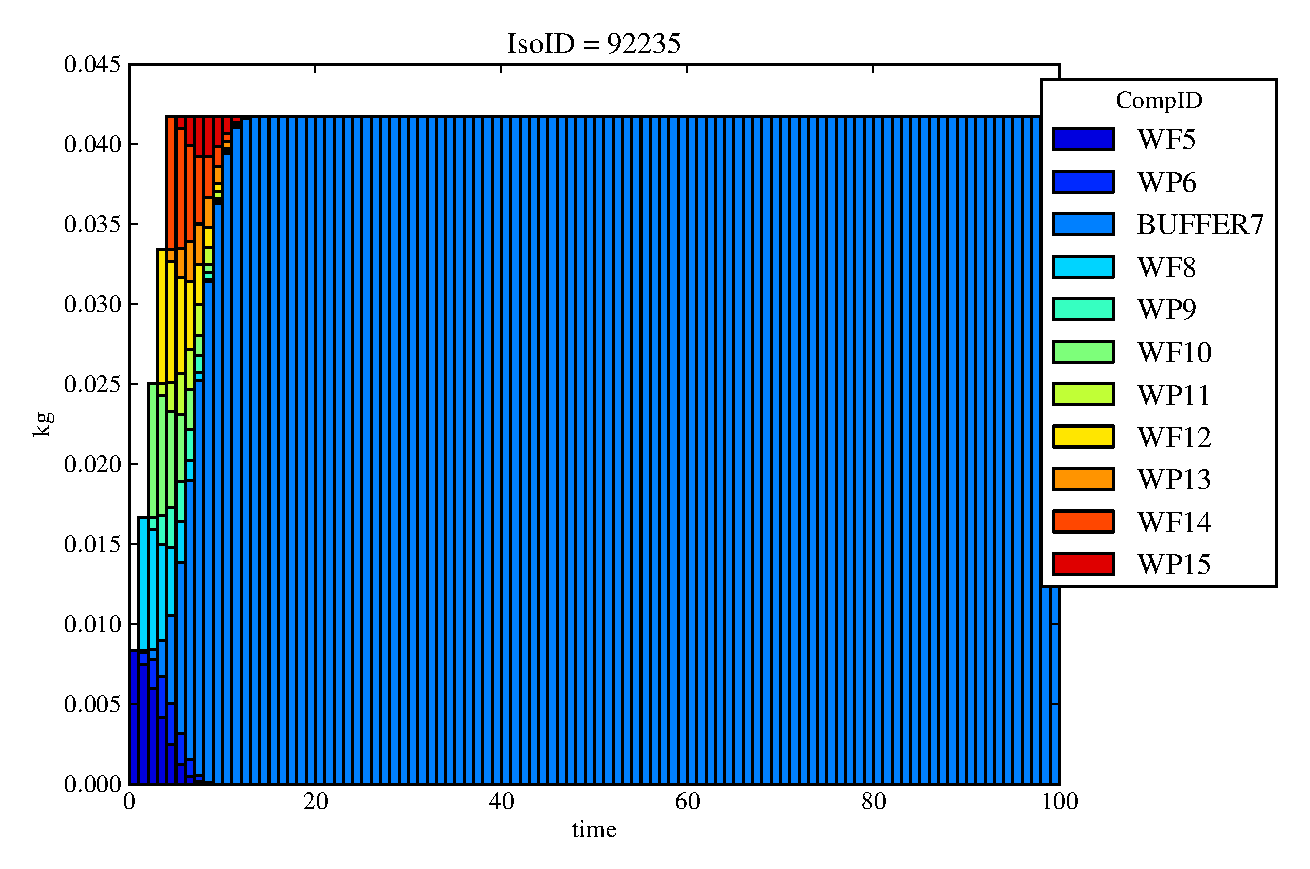
\includegraphics[width=0.8\textwidth]{./images/drIII.eps}
\caption[$^{235}U$ residence. Degradation Rate Buffer No Release.]{
For Case DRIII, in which total containment in the buffer is assumed ($F_{d,buffer}=0$), 
$^{235}U$ travels through waste forms and waste package components ($F_d = 0.1$) before 
permanent residence in the buffer component.
}
\label{fig:drIIIall}
\end{figure}
\end{frame}

\begin{frame}
  \frametitle{Degradation Rate Model Base Case III}
  \begin{figure}
\begin{minipage}[b]{0.45\linewidth}

  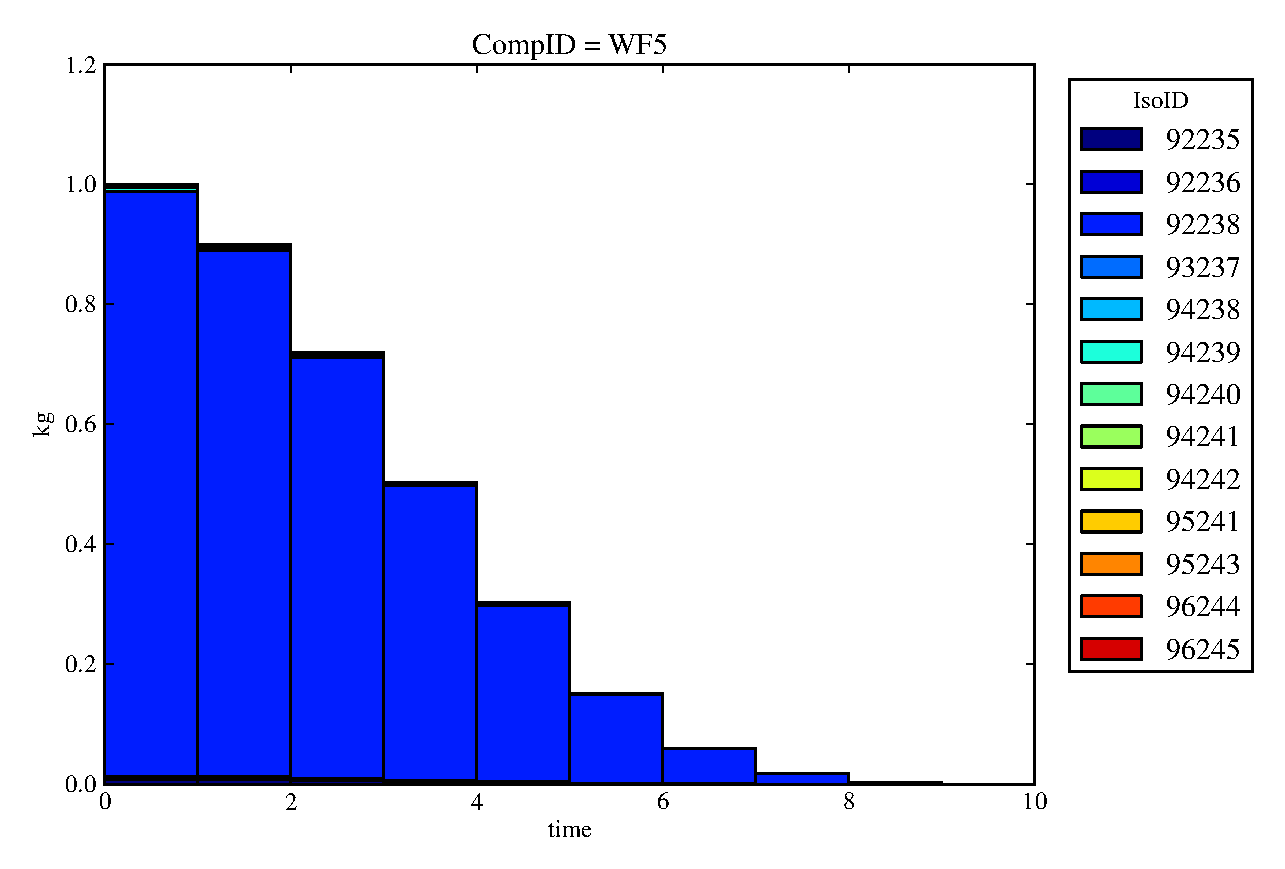
\includegraphics[width=0.8\textwidth]{./images/drIII1.eps}
  \caption[DRIII Waste Form Contaminants.]{
    Waste Form 5 ($F_d = 0.1$) releases material with degradation. 
    }
  \label{fig:drIIIwf5}
  
  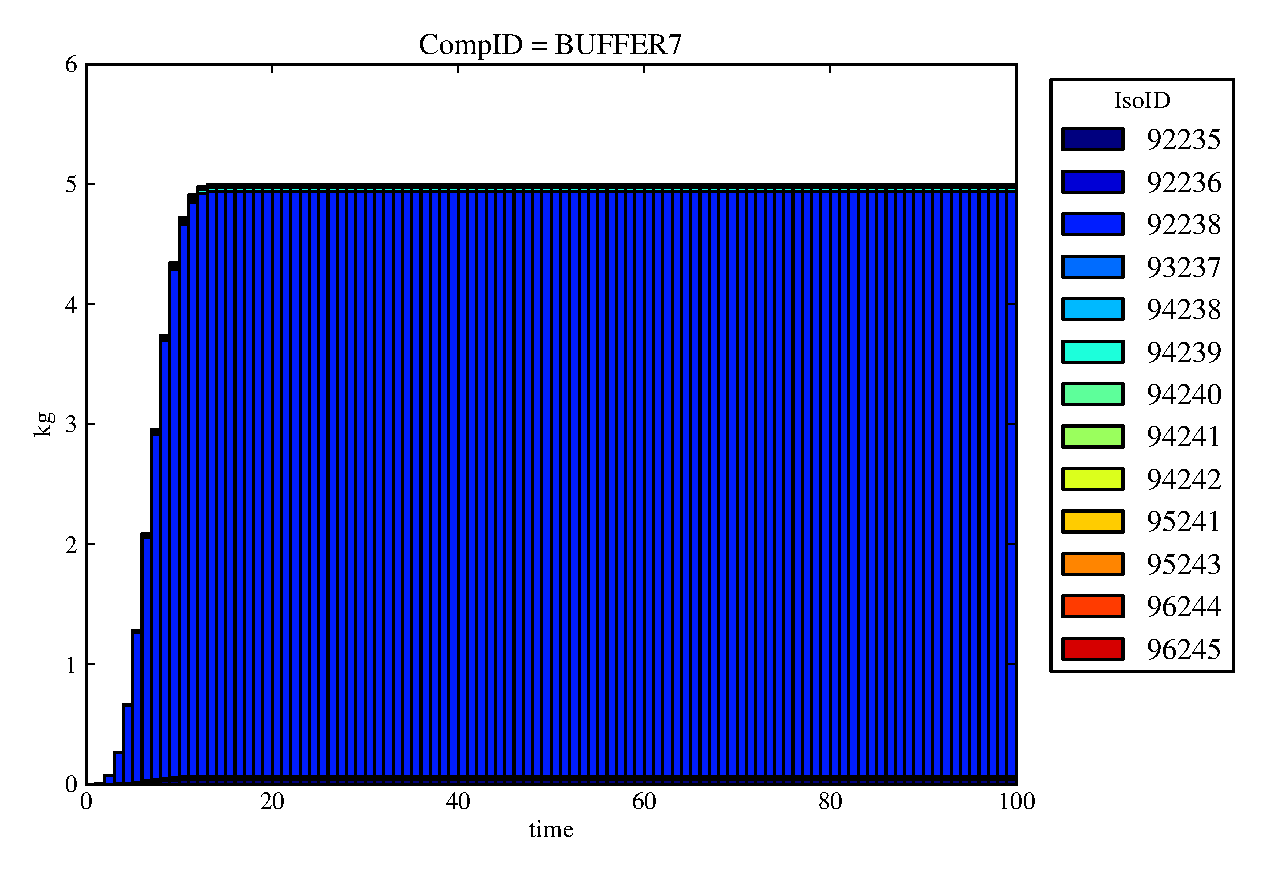
\includegraphics[width=0.8\textwidth]{./images/drIII3.eps}
  \caption[Case DRIII Buffer Contaminants]{
    Buffer 7 ($F_d=0$) acheives total containment.
    }
  \label{fig:drIIIbuff}

\end{minipage}
\hspace{0.05\linewidth}
\begin{minipage}[b]{0.45\linewidth}
  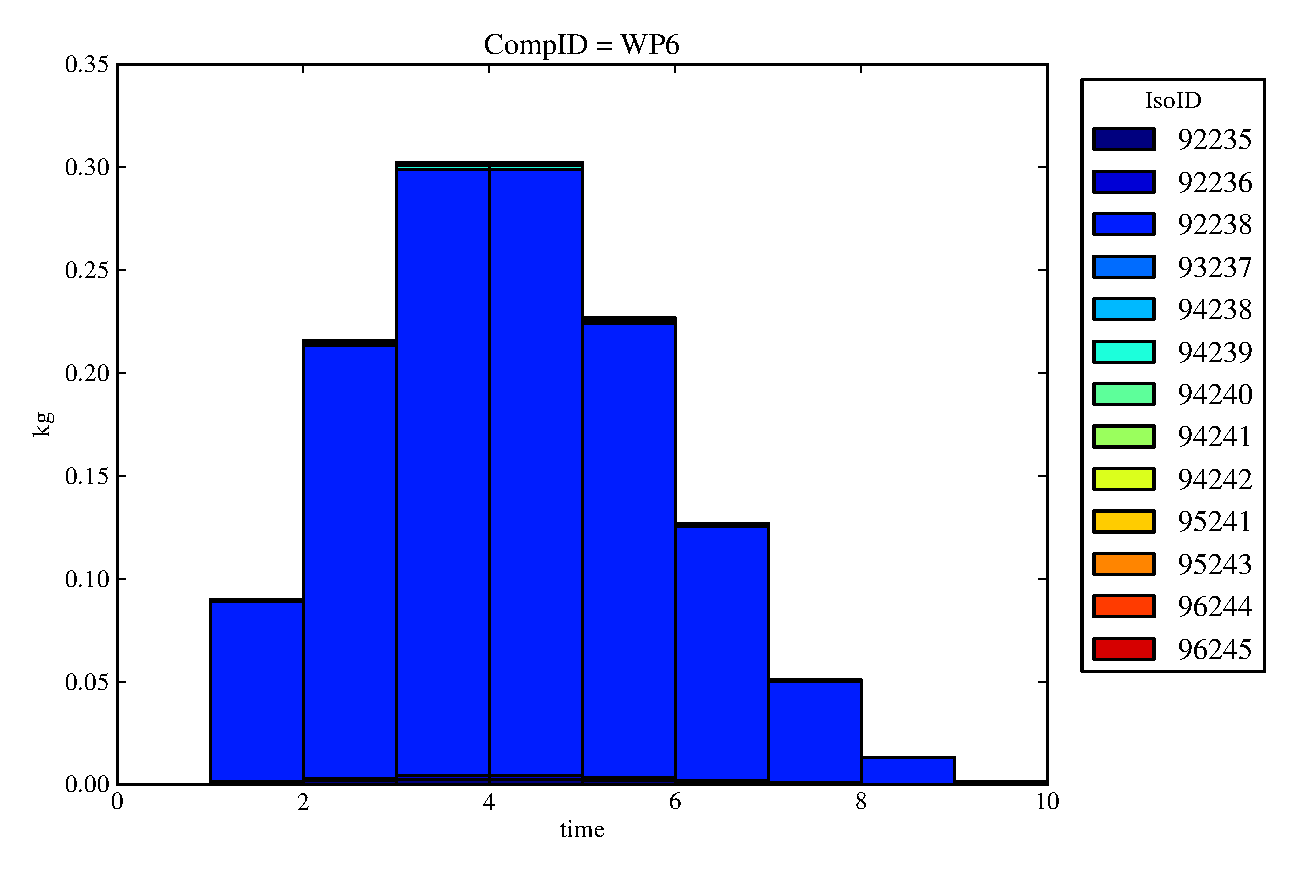
\includegraphics[width=0.8\textwidth]{./images/drIII2.eps}
  \caption[Case DRIII Waste Package Contaminants.]{ 
    Waste Package 6 ($F_d = 0.1$) receives and releases material. 
    }
  \label{fig:drIIIwp6}

  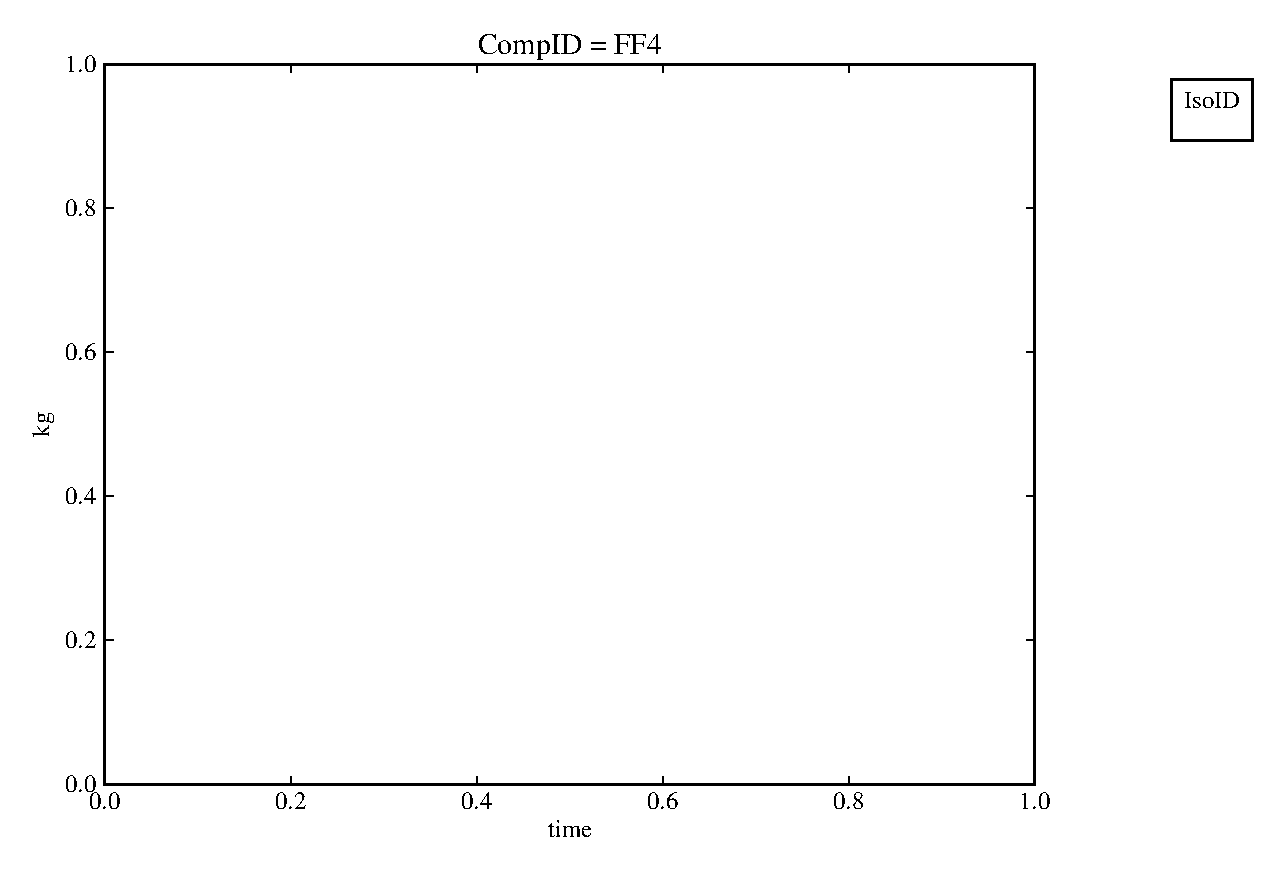
\includegraphics[width=0.8\textwidth]{./images/drIII0.eps}
  \caption[Case DRIII Waste Package Contaminants.]{ 
    Far Field 4 ($F_d = 0.1$), never receives material.
    }
  \label{fig:drIIIff0}


  \end{minipage}
\end{figure}
\end{frame}


\begin{frame}[ctb!]
  \frametitle{Degradation Rate Model Base Case IV}

\begin{figure}[ht]
\centering
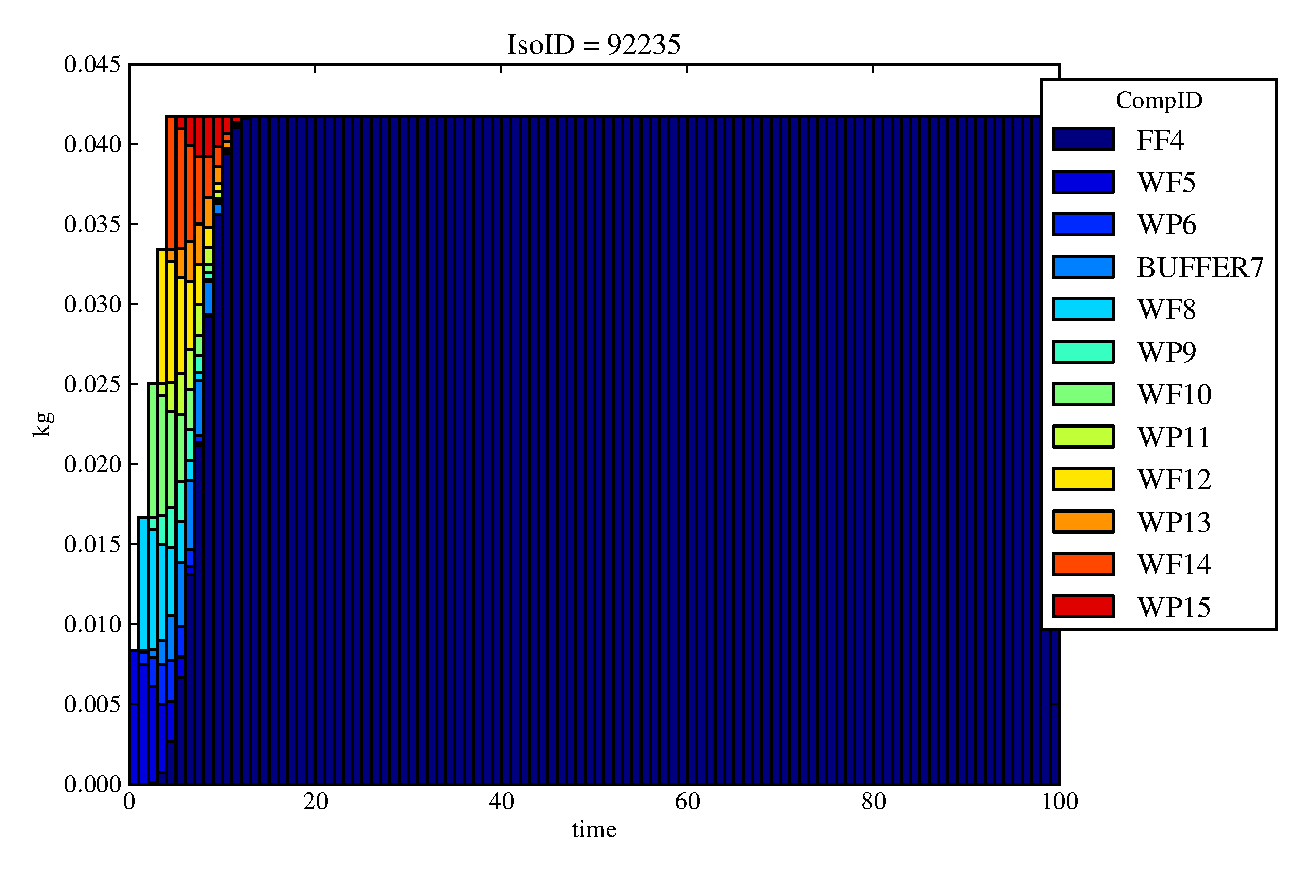
\includegraphics[width=0.8\textwidth]{./images/drIV.eps}
\caption[$^{235}U$ residence. Degradation Rate Buffer No Release.]{
For DRIV case in which total containment in the far field is assumed ($F_{d,ff}=0$), 
$^{235}U$ travels through interior components ($F_d = 0.1$) before 
permanent residence in the far field component.
}
\label{fig:drIVall}
\end{figure}
\end{frame}

\begin{frame}
  \frametitle{Degradation Rate Model Base Case IV}
  \begin{figure}
\begin{minipage}[b]{0.45\linewidth}

  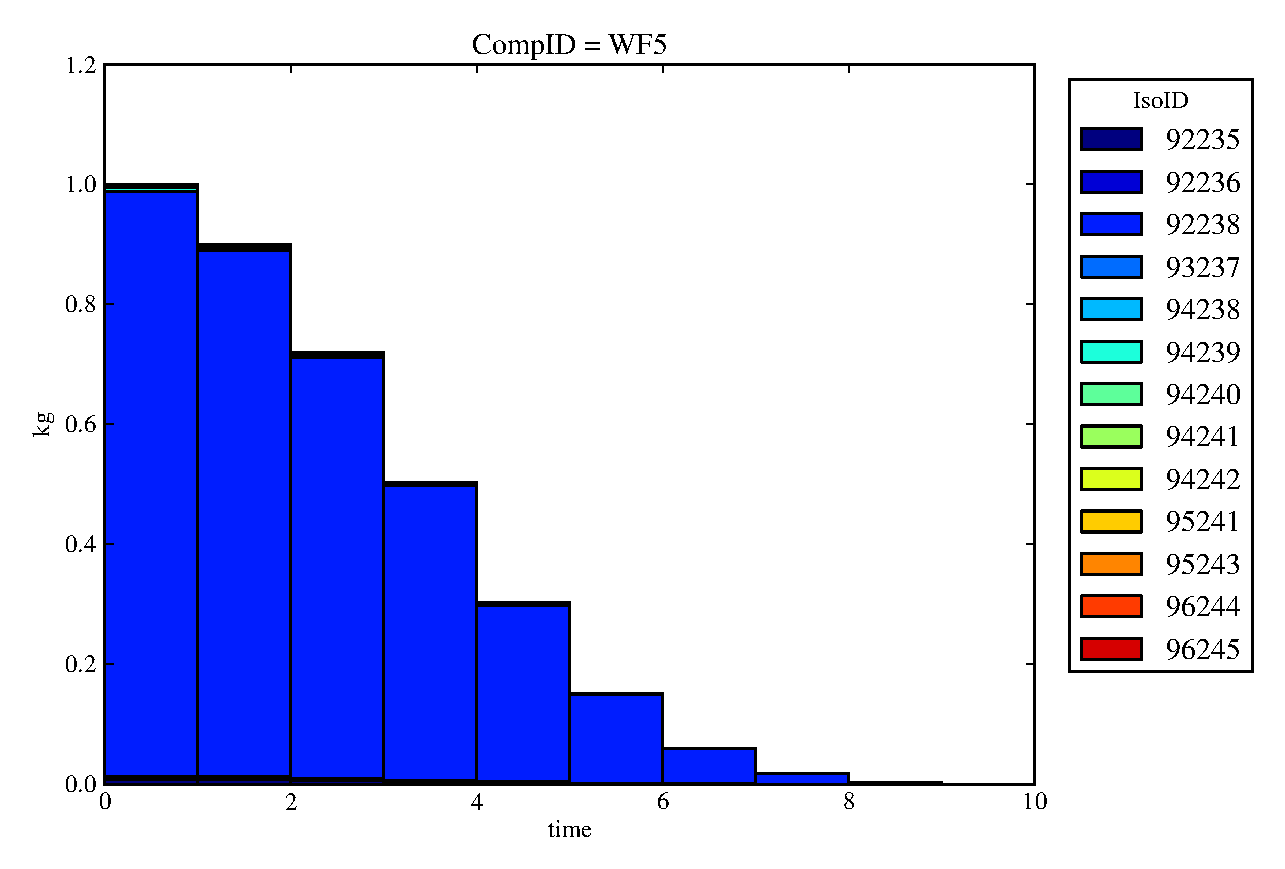
\includegraphics[width=0.8\textwidth]{./images/drIV1.eps}
  \caption[DRIV Waste Form Contaminants.]{
    Waste Form 5 ($F_d = 0.1$) releases material with degradation. 
    }
  \label{fig:drIVwf5}
  
  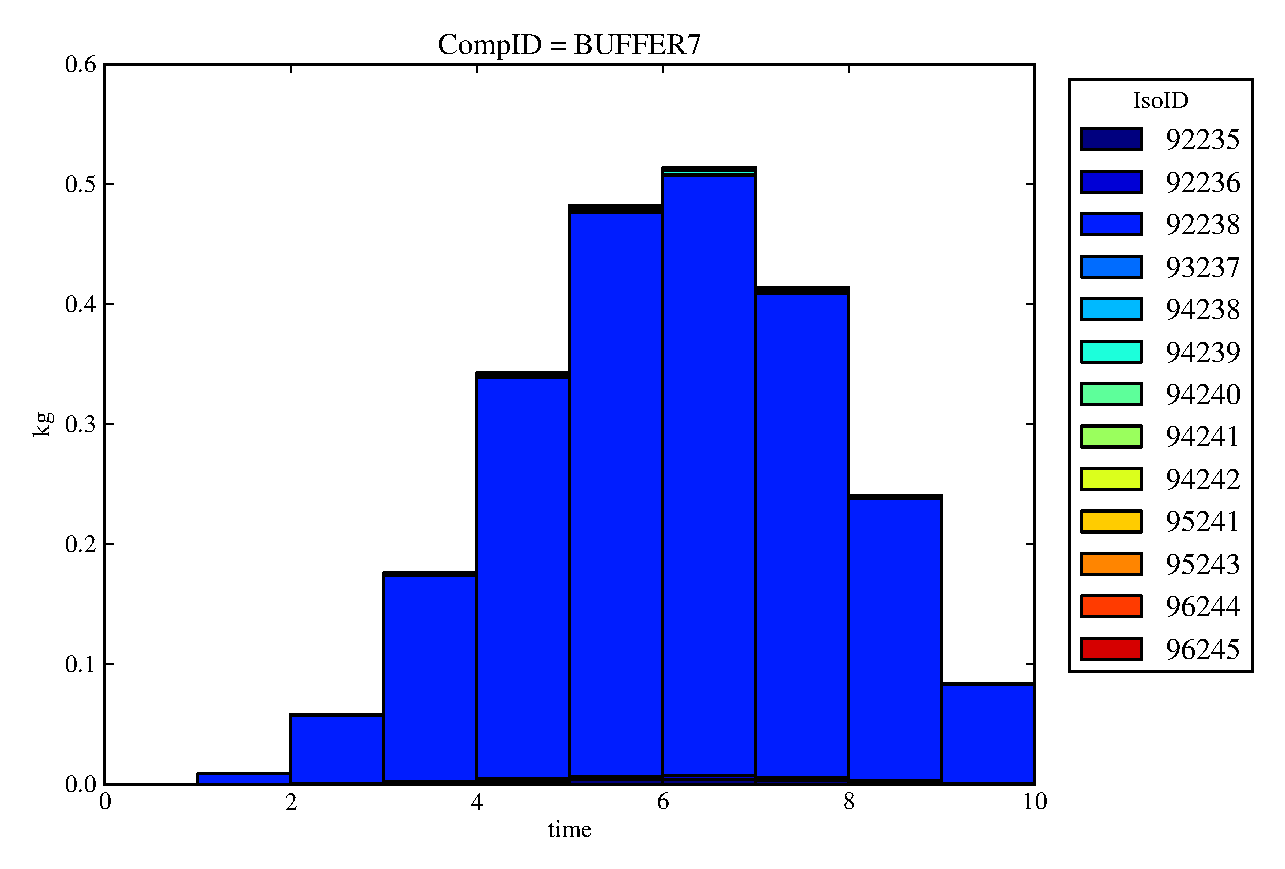
\includegraphics[width=0.8\textwidth]{./images/drIV3.eps}
  \caption[Case DRIV Buffer Contaminants]{
    The Buffer, component 7 ($F_d=0.0$), receives and then releases material.
    }
  \label{fig:drIVbuff}

\end{minipage}
\hspace{0.05\linewidth}
\begin{minipage}[b]{0.45\linewidth}
  \includegraphics[width=0.8\textwidth]{./images/drIV2.eps}
  \caption[Case DRIV Waste Package Contaminants.]{ 
    Waste Package 6 ($F_d = 0.1$) receives and releases material. 
    }
  \label{fig:drIVwp6}

  \includegraphics[width=0.8\textwidth]{./images/drIV0.eps}
  \caption[Case DRIV Waste Package Contaminants.]{ 
    Far Field 4 ($F_d = 0.0$), acheives total containment.
    }
  \label{fig:drIVff0}


  \end{minipage}
\end{figure}
\end{frame}

\begin{frame}[ctb!]
  \frametitle{Mixed Cell Model Base Case II}
  \begin{figure}
\begin{minipage}[b]{0.45\linewidth}

  \includegraphics[width=0.8\textwidth]{./images/mcIII1.eps}
  \caption[MCI WF Contaminants.]{
    WF 5 releases material with degradation. 
    }
  \label{fig:mcIIIwf5}
  
  \includegraphics[width=0.8\textwidth]{./images/mcIII3.eps}
  \caption[Case MCI Buffer Contaminants]{
    Buffer 7 ($F_d=0.1$), receives and releases material.
    }
  \label{fig:mcIIIbuff}

\end{minipage}
\hspace{0.05\linewidth}
\begin{minipage}[b]{0.45\linewidth}
  \includegraphics[width=0.8\textwidth]{./images/mcIII2.eps}
  \caption[Case MCI WP Contaminants.]{ 
    WP 6 receives and releases material. 
    }
  \label{fig:mcIIIwp6}

  \includegraphics[width=0.8\textwidth]{./images/mcIII0.eps}
  \caption[Case MCI WP Contaminants.]{ 
    Far Field 4 acheives total containment.
    }
  \label{fig:mcII}


  \end{minipage}
\end{figure}

\end{frame}


\begin{frame}[ctb!]
  \frametitle{Mixed Cell Model Base Case II}
\begin{figure}[ht]
\centering
\includegraphics[width=0.8\textwidth]{./images/mcIII.eps}
\caption[$^{235}U$ residence. Mixed Cell Coupled Sorption and Solubility Limitation.]{
For the MCII case in which containment is affected by both sorption and 
solubility limitation,
($F_{d}=0.1$, $S_{ref}=0.1kg/m^3$ for all components), $^{235}U$ travels more slowly
before permanent residence in the far field component.
}
\label{fig:mcIIIall}
\end{figure}
\end{frame}



\begin{frame}[ctb!]
\begin{figure}[ht]
\centering
\includegraphics[width=0.8\textwidth]{./chapters/demonstration/base/lpDM_t_t.eps}
\caption[Lumped Parameter Dispersion Model Transit Time Sensitivity]{The transit time 
parameterization of the lumped parameter dispersion model of radionuclide 
transport has a strong effect on the material reaching the far field after 30 
years.  }
\label{fig:lp_t_t_begin}
\end{figure}
\end{frame}

\begin{frame}[ctb!]
\begin{figure}[ht]
\centering
\includegraphics[width=0.8\textwidth]{./chapters/demonstration/base/lpEXPM_t_t.eps}
\caption[Lumped Parameter Exponential Model Transit Time Sensitivity]{The transit time 
parameterization of the lumped parameter exponential model of radionuclide 
transport has a strong effect on the material reaching the far field after 30 
years.  }
\end{figure}
\end{frame}

\begin{frame}[ctb!]
\begin{figure}[ht]
\centering
\includegraphics[width=0.8\textwidth]{./chapters/demonstration/base/lpPFM_t_t.eps}
\caption[Lumped Parameter Piston Flow Model Transit Time Sensitivity]{The transit time 
parameterization of the lumped parameter piston flow model of radionuclide 
transport has a strong effect on the material reaching the far field after 30 
years.  }
\label{fig:lp_t_t_end}
\end{figure}
\end{frame}

\begin{frame}[ctb!]
  \frametitle{One Dimensional Permeable Porous Medium Base Case}
\begin{figure}[ht]
\includegraphics[width=0.8\textwidth]{./chapters/demonstration/base/1dppmff.eps}
\caption[$^{235}U$ residence 1 Dimensional PPM Model.]{
For the case in which transport through the waste form, waste package, and 
buffer are represented by quickly degrading Mixed Cell models and the Far Field 
is represented by the 1 Dimensional PPM model, material moves very slowly into 
the far field. These results demonstrate numerical difficulties in timestep 10, 
despite overloading this simulation with 1,000,000 initial kg per waste form.
}
\label{fig:1dppmall}
\end{figure}
\end{frame}


\subsection{Radionuclide Transport Validation Cases}
\begin{frame}[ctb!]
  \frametitle{Radionuclide Transport Validation Demonstrations}
\end{frame}

\subsection{Thermal Transport Toy Cases}
\begin{frame}[ctb!]
  \frametitle{Thermal Base Case Demonstration}
\end{frame}

\subsection{Thermal Transport Validation Cases}

\subsection{Waste Package Spacing Sensitivity Validation}\label{sec:spacing}
The waste package spacing, $s$ of geologic repository concept effects the areal 
decay heat burden in the repository and has a strong effect on the thermal 
energy deposited per unit area in the medium. 

\subsubsection{LLNL Model Results}

In the creation of the \gls{STC} database, the waste package spacing was varied 
across a number of values for each isotope, $i$, limiting 
radius $r_{calc}$, thermal diffusivity $\alpha_{th}$, and thermal conductivity $K_{th}$, considered.  By 
varying the waste package spacing of the geometric layout from $0.1-5 [m]$
this sensitivity analysis succeeds in capturing the domain of 
waste package spacings present in geologic repository concepts under 
consideration. 

\begin{figure}[htbp!]
\begin{center}
\includegraphics[width=\columnwidth]{./thermal_demonstration/spacing/Cm242spacing_sens.eps}
\end{center}
\caption[$K_{th}$ Sensitivity to $s$]{Increased waste package 
spacing decreases areal thermal energy deposition 
(here represented by \gls{STC}) in the near field (here $r_{calc} = 0.5m$).}
\label{fig:Cm242spacing_sens}
\end{figure}

Figure \ref{fig:Cm242spacing_sens} shows the trend in which increased waste package spacing of a medium decreases areal thermal energy 
deposition in the near field. This indicates that waste package spacing is 
an important parameter for repository concept design.

Similarly, the location of the limiting radius has a strong effect on the 
waste package loading limit, for a fixed limiting temperature. In Figure 
\ref{fig:Cm242r_lim_sens}, the trend is demonstrated in which increased limiting 
radius decreases the thermal energy contributing to the thermal limit. 


\begin{figure}[htbp!]
\begin{center}
\includegraphics[width=\columnwidth]{./thermal_demonstration/spacing/Cm242r_lim_sens.eps}
\end{center}
\caption[$K_{th}$ Sensitivity to $r_{lim}$]{Increased limiting radius 
decreases thermal energy deposition contributing to the thermal limit
(here represented by \gls{STC}).}
\label{fig:Cm242r_lim_sens}
\end{figure}


\subsubsection{Cyder Results}

In a similar analysis, the thermal diffusivity was compared both with the 
spacing between waste packages and the limiting radius. 

Figure \ref{fig:rs} validates the trend noted above that 
increased waste package spacing in a repository concept decreases areal thermal energy deposition 
in the near field.  Additionally, analysis with the \Cyder STC database 
demonstrates the way in which the importance of $r_{lim}$, the limiting radius, 
impacts the maximum calculated temperature at that radius. 


\begin{figure}[htbp!]
\begin{center}
\includegraphics[width=\columnwidth]{./thermal_demonstration/spacing/rs.eps}
\end{center}
\caption[$\alpha_{th}$ vs. $r_{lim}$ Sensitivity in Cyder]
{Cyder results agree with 
those of the LLNL model. The importance of the limiting radius decreases with 
increased $K_{th}$. The above example thermal profile results from 10kg of 
$^{242}Cm$}
\label{fig:rs}
\end{figure}



\begin{frame}[ctb!]
\frametitle{LLNL Model Thermal Conductivity Sensitivity}

\begin{figure}[htbp!]
\begin{center}
\includegraphics[height=0.7\textheight]{./thermal_demonstration/conductivity/conductivity.eps}
\end{center}
\caption[$K_{th}$ Sensitivity in LLNL Model]{Increased thermal conductivity decreases thermal energy deposition 
(here represented by STC) in the near field (here $r_{calc} = 0.5m$).}
\label{fig:Cm242Kth_alpha_low}
\end{figure}

\end{frame}


\begin{frame}[ctb!]
\frametitle{Cyder Thermal Conductivity Sensitivity}
\begin{figure}[htbp!]
\begin{center}
\includegraphics[height=0.7\textheight]{./thermal_demonstration/conductivity/conductivity.eps}
\end{center}
\caption[$K_{th}$ Sensitivity in Cyder]
{Cyder results agree with those of the LLNL model. Increased $K_{th}$ decreases 
thermal energy deposition at the limiting radius. The above example thermal 
profile results from 10kg of $^{242}Cm$, $\alpha_{th}=$, $s=$, and $r_{lim}=$.}
\label{fig:kr}
\end{figure}
\end{frame}

%\begin{frame}[ctb!]
%\frametitle{Cyder Thermal Conductivity and Limiting Radius Sensitivity}
%\begin{figure}[htbp!]
%\begin{center}
%\includegraphics[height=0.7\textheight]{./thermal_demonstration/conductivity/kr.eps}
%\end{center}
%\caption[$K_{th}$ vs. $r_{lim}$ Sensitivity in Cyder]
%{Cyder results agree with 
%those of the LLNL model. The importance of the limiting radius decreases with 
%increased $K_{th}$. The above example thermal profile results from 10kg of 
%$^{242}Cm$}
%\label{fig:kr}
%\end{figure}
%\end{frame}


%\begin{frame}[ctb!]
%\frametitle{Cyder Thermal Conductivity and Limiting Radius Sensitivity}
%\begin{figure}[htbp!]
%\begin{center}
%\includegraphics[height=0.7\textheight]{./thermal_demonstration/conductivity/ks.eps}
%\end{center}
%\caption[$K_{th}$ vs. Waste Package Spacing Sensitivity in Cyder]{Cyder results agree with 
%those of the LLNL model. The importance of the limiting radius decreases with 
%increased $K_{th}$. The above example thermal profile results from 10kg of 
%$^{242}Cm$}
%\label{fig:ks}
%\end{figure}
%\end{frame}


\begin{frame}[ctb!]
\frametitle{LLNL Model Thermal Diffusivity Sensitivity}
\begin{figure}[htbp!]
\begin{center}
\includegraphics[height=0.7\textheight]{./thermal_demonstration/diffusivity/diffusivity.eps}
\end{center}
\caption[$K_{th}$ Sensitivity to $\alpha_{th}$]{Increased thermal 
diffusivity decreases temperature change (here represented by STC) at the 
limiting radius (here $r_{calc} = 0.5m$).}
\label{fig:Cm242alpha_kth_low}
\end{figure}
\end{frame}

\begin{frame}[ctb!]
\frametitle{Cyder Thermal Diffusivity Sensitivity}
\begin{figure}[htbp!]
\begin{center}
\includegraphics[height=0.7\textheight]{./thermal_demonstration/diffusivity/diffusivity_cyder.eps}
\caption[$\alpha_{th}$ Sensitivity in Cyder]{Cyder trends agree with those of 
the LLNL model, in which increased thermal diffusivity results in reduced 
temperature change at the limiting radius. The above example thermal profile 
results from 10kg of $^{242}Cm$.} 
\label{fig:ar}
\end{center}
\end{figure}
\end{frame}

%\begin{frame}[ctb!]
%\frametitle{Cyder Thermal Diffusivity and Conductivity Sensitivity}
%\begin{figure}[htbp!]
%\begin{center}
%\includegraphics[height=0.7\textheight]{./thermal_demonstration/diffusivity/ak.eps}
%\caption[$\alpha_{th}$ vs. $K_{th}$ Sensitivity in Cyder]{Cyder trends agree 
%with those of the LLNL model, in which increased thermal diffusivity results in 
%decreased thermal depsoition in the near field. The above example thermal 
%profile results from 10kg of $^{242}Cm$.} 
%\label{fig:ar}
%\end{center}
%\end{figure}
%\end{frame}
%
%\begin{frame}[ctb!]
%\frametitle{Cyder Thermal Diffusivity and Limiting Radius Sensitivity}
%\begin{figure}[htbp!]
%\begin{center}
%\includegraphics[height=0.7\textheight]{./thermal_demonstration/diffusivity/ar.eps}
%\end{center}
%\caption[$\alpha_{th}$ vs. $r_{lim}$ Sensitivity in Cyder]
%{Cyder trends agree with those of the LLNL model. The importance of the 
%limiting radius decreases with increased $K_{th}$. The above example thermal 
%profile results from 10kg of $^{242}Cm$.}
%\label{fig:ak}
%\end{figure}
%\end{frame}
%



\section{Conclusion}

\begin{frame}[ctb!]
  \frametitle{Conclusion : Summary of Contributions}
\end{frame}

\begin{frame}[ctb!]
  \frametitle{Conclusion : Suggested Future Work}
\end{frame}



\begin{frame}[ctb!]
  \frametitle{Acknowledgements}  
  My work at Argonne is supported by the Office of Science Laboratory graduate 
  program, the Used Fuel Disposition Campaign, and my supervisor Mark Nutt.

   etc.
\end{frame}

%%--------------------------------%%
%%--------------------------------%%
\begin{frame}[allowframebreaks]
  \frametitle{References}
  \bibliographystyle{plain}
  {\footnotesize \bibliography{defense} }

\end{frame}

%%--------------------------------%%


\appendix
\newcounter{finalframe}
\setcounter{finalframe}{\value{framenumber}}
\section{LLNL Model Background}
% LLNL
\subsection{Analytical Model Background}
\begin{frame}[ctb!]
\frametitle{Analytical Model : Background}
The analytical  model
\begin{itemize} 
  \item was created at LLNL (H. Greenberg, J. Blink, et. al) \cite{hardin_generic_2011, sutton_investigations_2011, 
greenberg_application_2012}
  \item employs an analytic model from Carslaw and Jaeger \cite{carslaw_conduction_1959} 
  \item is implemented in MathCAD \cite{ptc_mathcad_2010}
  \item seeks to inform heat limited waste capacity calculations for 
    \begin{itemize}
      \item arbitrary geology 
      \item arbitrary waste package loading densities
      \item arbitrary homogeneous decay heat source
    \end{itemize}
\end{itemize}
\end{frame}

\begin{frame}
  \frametitle{Analytical Model : Geometry}
  \begin{figure}[h!]
    \begin{center}
      \includegraphics[width=0.7\textwidth]{./images/llnlConcept.eps}
    \end{center}
    \caption{Vertical, horizontal, alcove, and borehole emplacement layouts can 
    be represented by a line of point sources and adjacent line sources 
    \cite{sutton_investigations_2011}.}
    \label{fig:llnl}
  \end{figure}
\end{frame}

\begin{frame}
  \frametitle{Analytical Model : Calculation Method}
    LLNL's model is a MathCAD solution of the transient homogeneous 
    conduction equation,
    \begin{align}
      \nabla^2T  = \frac{1}{\alpha}\frac{\partial T}{\partial t},
      \label{condGl}
    \end{align}
    in which superimposed point and line source solutions approximate the repository 
    layout.
\end{frame}

\begin{frame}[ctb!]
\frametitle{Analytical Model : Calculation Method}
The model consists of two conceptual regions, an external region representing 
the host rock and an internal region representing the waste form, package, and 
buffer Engineered Barrier System within the disposal tunnel wall.   
\begin{itemize}
  \item Since the thermal mass of the EBS is small in comparison to the thermal 
    mass of the host rock, the internal region may be treated as quasi-steady 
    state.
  \item The transient state of the temperature at the calculation radius is 
    found with a convolution of the transient external solution with the steady 
    state internal solution.
  \item The internal and external regions are \textbf{approximated} to be a 
    single homogeneous medium.
  \item The process is then iterated with a one year resolution in order to 
    arrive at a temperature evolution over the lifetime of the repository. 
\end{itemize}
\end{frame}


\begin{frame}[ctb!]
\frametitle{Analytical Model : Calculation Method}
\begin{minipage}{0.3\textwidth}
\begin{figure}[h!]
  \begin{center}
    \includegraphics[width=\textwidth]{./images/llnlConcept.eps}
  \end{center}
  \caption{The central package is represented by a finite line source
  \cite{sutton_investigations_2011}.}
  \label{fig:llnl}
\end{figure}
\end{minipage}
\hspace{0.01mm}
\begin{minipage}{0.6\textwidth}
The geometric layout of the analytic LLNL model in Figure \ref{fig:llnl} 
shows  that the central package is represented by the finite line solution
\footnotesize{
\begin{align}
  T_{line}&(t,x,y,z) = \nonumber\\
  &\frac{1}{8\pi K_{th}} 
  \bigintsss_0^t\!\frac{q_L(t')}{t-t'}e^{ \frac{-\left(x^2 + z^2\right)}{4\alpha 
  (t-t')} }\nonumber\\ &\cdot\left[ \erf{\left[ \frac{1}{2} \frac{\left( y + 
  \frac{L}{2} \right)}{\sqrt{\alpha(t-t')}}  \right]} - \erf{\left[ \frac{1}{2} 
  \frac{\left( y - \frac{L}{2} \right)}{\sqrt{\alpha(t-t')}}  \right]} 
  \right]\,\mathrm{dt'}.
  \label{line}
\end{align}
}
\end{minipage}
\end{frame}

\begin{frame}[ctb!]
\frametitle{Analytical Model : Calculation Method}
\begin{minipage}{0.3\textwidth}
\begin{figure}[h!]
  \begin{center}
    \includegraphics[width=\textwidth]{./images/llnlConcept.eps}
  \end{center}
  \caption{Adjacent packages are represented as point sources
  \cite{sutton_investigations_2011}.}
  \label{fig:llnl}
\end{figure}
\end{minipage}
\hspace{0.1mm}
\begin{minipage}{0.6\textwidth}
 Adjacent packages within the central tunnel are represented by the point source 
 solution,
 \footnotesize{
  \begin{align}
    T_{point}(t,r) &= \frac{1}{8K_{th}\sqrt{\alpha}\pi^{\frac{3}{2}}}\nonumber\\
     &\bigintsss_0^{t}\!\frac{q(t')}{(t-t')^{\frac{3}{2}}}e^{\frac{-r^2}{4\alpha(t-t')}}\,\mathrm{dt'}.
    \label{point}
  \end{align}
  }
  \end{minipage}
\end{frame}


\begin{frame}[ctb!]
\frametitle{Analytical Model : Calculation Method}
\begin{minipage}{0.3\textwidth}
\begin{figure}[h!]
  \begin{center}
    \includegraphics[width=\textwidth]{./images/llnlConcept.eps}
  \end{center}
  \caption{The non-central disposal tunnels are represented as infinite line sources
  \cite{sutton_investigations_2011}.}
  \label{fig:llnl}
\end{figure}
\end{minipage}
\hspace{0.1mm}
\begin{minipage}{0.6\textwidth}
Adjacent disposal tunnels are represented by the infinite line source solution,
\footnotesize{
\begin{align}
  T_{\infty line}(t,x,z) &= \frac{1}{4\pi K_{th}} 
  \bigintsss_0^t\frac{q_L(t')}{t-t'}e^{ \frac{-\left(x^2 + z^2\right)}{4\alpha 
  (t-t')} }
  \label{infline}
  \intertext{in infinite homogeneous media, where}
  \alpha &= ~~\mbox{thermal diffusivity } [m^2\cdot s^{-1}]\nonumber\\
  q(t) &= ~~\mbox{point heat source} [W]\nonumber\\
  \intertext{and}
  q_L(t) &= ~~\mbox{linear heat source} [W\cdot m^{-1}]\nonumber
\end{align}
}
Superimposed point and line source solutions allow for a notion of the 
repository layout to be modeled in the host rock.
\end{minipage}
\end{frame}



\section{Geologic Media and Concepts}
\begin{frame}[ctb!]
  \frametitle{Clay Disposal Environments}
  \footnotesize{

  \begin{figure}[h!]
    \begin{center}
      \includegraphics[height=.7\textheight]{./images/belgianClayRedImp.eps}
    \end{center}
    \caption{Belgian reference concept in Boom Clay 
    \cite{von_lensa_red-impact_2008}.}
    \label{fig:belgianClayRedImp}
  \end{figure}

}
\end{frame}

\begin{frame}[ctb!]
  \frametitle{Granite Disposal Environments}
  \footnotesize{

  \begin{figure}[h!]
    \begin{center}
      \includegraphics[height=.7\textheight]{./images/czechGraniteRedImp.eps}
    \end{center}
    \caption{Czech reference concept in Granite 
    \cite{von_lensa_red-impact_2008}.}
    \label{fig:czechGraniteRedImp}
  \end{figure}
}
\end{frame}

\begin{frame}[ctb!]
  \frametitle{Salt Disposal Environments}
  \footnotesize{

  \begin{figure}[h!]
    \begin{center}
      \includegraphics[height=.7\textheight]{./images/carter_salt_layout.eps}
    \end{center}
    \caption{DOE-NE Used Fuel Disposition Campaign  concept in 
    Salt \cite{hardin_generic_2011}.}
    \label{fig:salt_layout}
  \end{figure}
}
\end{frame}
\begin{frame}[ctb!]
  \frametitle{Salt Disposal Environments}
  \footnotesize{

  \begin{figure}[h!]
    \begin{center}
      \includegraphics[height=.7\textheight]{./images/hardin_salt_layout.eps}
    \end{center}
    \caption{DOE-NE Used Fuel Disposition Campaign  concept in 
    Salt \cite{hardin_generic_2011}.}
    \label{fig:hardin_salt_layout}
  \end{figure}
}
\end{frame}

\begin{frame}[ctb!]
  \frametitle{Deep Borehole Disposal Environment}
  \footnotesize{

  \begin{figure}[h!]
    \begin{center}
      \includegraphics[height=.7\textheight]{./images/boreholeGPAM.eps}
    \end{center}
    \caption{DOE-NE Used Fuel Disposition Campaign Deep Borehole concept 
    \cite{hardin_generic_2011}.}
    \label{fig:boreholeGPAM}
  \end{figure}
}
\end{frame}

%%----------------------------------------%%
\begin{frame}[ctb!]
  \frametitle{Engineered Barriers : Waste Forms}
\footnotesize{
  The first line of defense is the waste form.
  \begin{figure}[htbp!]
  \begin{center}
    \includegraphics[width=0.5\textwidth]{./images/waste_forms_poinssot.eps}
  \end{center}
  \caption{A comparison of uranium oxide and borosilicate glass waste forms 
  \cite{poinssot_long-term_2012}.}
  \label{fig:waste_forms_poinssot}
\end{figure}

}
\end{frame}

%%----------------------------------------%%
\begin{frame}[ctb!]
  \frametitle{Engineered Barriers : Waste Packages}
\footnotesize{
  \begin{figure}[htbp!]
  \begin{center}
    \includegraphics[width=0.7\textwidth]{./images/packages_ineel.eps}
  \end{center}
  \caption{Conceptual mockup of waste packages around waste forms 
    \cite{bridges_standardized_2001}.}
  \label{fig:packages}
\end{figure}

}
\end{frame}

%%----------------------------------------%%
\begin{frame}[ctb!]
  \frametitle{Engineered Barriers : Disposal Cask}
\footnotesize{
  \begin{figure}[htbp!]
  \begin{center}
    \includegraphics[width=0.7\textwidth]{./images/cask_ineel.eps}
  \end{center}
  \caption{Conceptual mockup of a transport and disposal cask 
    \cite{bridges_standardized_2001}.}
  \label{fig:packages}
\end{figure}

}
\end{frame}

%%----------------------------------------%%
\begin{frame}[ctb!]
  \frametitle{Engineered Barriers : Buffer}
\footnotesize{
  \begin{figure}[h!]
    \begin{center}
      \includegraphics[height=.7\textheight]{./images/belgianClayRedImp.eps}
    \end{center}
    \caption{Belgian reference concept in Boom Clay 
    \cite{von_lensa_red-impact_2008}.}
    \label{fig:belgianClayRedImp}
  \end{figure}
}
\end{frame}

%%----------------------------------------%%
\begin{frame}[ctb!]
  \frametitle{Natural Barrier : Geology}
\footnotesize{
  \begin{figure}[htbp!]
  \begin{center}
    \includegraphics[width=0.7\textwidth]{./images/wipp_stratigraph.eps}
  \end{center}
  \caption{The Waste Isolation Pilot Plant has many geologic layers above the 
    salt bed \cite{doe_wipp_2013}.}
  \label{fig:wipp}
\end{figure}

}
\end{frame}
\setcounter{framenumber}{\value{finalframe}}


\end{document}



